\documentclass[12pt]{article}  % Tipo de documento (puede ser book, report, etc.)

\usepackage[utf8]{inputenc}  % Codificación de caracteres (UTF-8)
\usepackage{amsmath, amssymb} % Paquetes para expresiones matemáticas
\usepackage{graphicx} % Para insertar imágenes
\usepackage[spanish]{babel} %Optimiza el typesetting para documentos en español
\usepackage[letterpaper, left=1in, right=1in, top=1in, bottom=1in]{geometry} %Para abarcar más hoja horizontalmente
\usepackage{booktabs} %Optimiza trabajar con tablas y agrega algunos comandos
\usepackage{multirow} %Para crear celdas tabulares que abarcan múltiples filas
\usepackage{float} %Mayor control donde se colocan las figuras y tablas
\usepackage{caption} %Mayor control de las captions de figuras y tablas
\usepackage{colortbl}%Para colores en tablas
\usepackage{xcolor} % Opcional, pero útil para definir colores personalizados
\definecolor{paleYellow}{RGB}{255, 255, 180} % Amarillo pálido

\title{Reporte de Tareas y Ejercicios Parcial 2}  % Título
\author{Suárez Saldaña, Jorge Alberto \\ Matrícula: 355992 \\[1ex] Materia: Modelado matemático \\ Profesor Reyes Castillo Rito}  % Autor
\date{\today}  % Fecha (puedes poner una específica)

\begin{document}
\maketitle
En este segundo parcial continuamos con el estudio de la resolución de problemas Programación Lineal o Investigación de Operaciones, en este caso, haciendo énfasis en los problemas relacionados a el \textbf{transporte}, transbordo y asignación de recursos.
Este tipo de problemas tienen en común la generación de recursos en un lugar (oferta) que deben ser transportados (con un costo) a lugares que requieren de estos recursos (demanda).
El objetivo consiste en determinar un modelo que minimice el costo total del transporte y que al mismo tiempo satisfaga los límites de oferta y demanda.
En estos modelos se supone que el costo de transporte es proporcional a la cantidad de unidades transportadas en determinada ruta.
El problema general se representa en una red, donde hay X fuentes y Y destinos, cada fuente y destino se representan con un nodo. Las rutas que enlazan las fuentes y destinos se representan con una arista.
Cada arco une a la fuente i con el destino j, lo que conlleva dos datos importante; el costo de transportar una unidad, y la cantidad transportada.
La cantidad de artículos ofertados desde las fuentes debe conincidir con la demandada por los destinos: \mbox{Oferta = demanda}.\\
En general, se puede ampliar el modelo de transporte a otras áreas de operación , como el control de inventarios, programación de empleos o asignación de personal.
Para encontrar la solución a este tipo de problemas, podemos usar herramientas como \mbox{\textit{LINGO}} o el \mbox{\textit{solver}} de \mbox{Microsoft Excel}.\\ A continuación, se detallan los problemas que se resolvieron como parte del segundo parcial de la materia de Modelado Matemático.

\section{Transporte de automóviles}
Una empresa tiene tres fábricas de autos: SLP, QRO y GTO; y los envía a MTY y CDMX en las cantidades constradas en las siguientes tablas:

%Recuerda que table es el entorno flotante y tabular crea la tabla
\begin{table}[H]
    \centering
    \begin{minipage}{0.40\textwidth} % Usa minipaginas para alienar horizontalmente las tablas
        \centering
        \caption{Costo de trasporte x auto}
        \label{tab:costoProb1}
        \begin{tabular}{ccc}
            & MTY & CDMX \\
            SLP & \$80 & \$215 \\
            QRO & \$100 & \$180 \\
            GTO & \$102 & \$68 \\
        \end{tabular}
    \end{minipage}
    \hfill % Espacio flexible entre tablas
    \begin{minipage}{0.25\textwidth}
        \centering
        \caption{Producción}
        \label{tab:oferProb1}
        \begin{tabular}{cc}
            SLP & 1000 \\
            QRO & 1500 \\
            GTO & 2000 \\
        \end{tabular}
    \end{minipage}
    \hfill
    \begin{minipage}{0.28\textwidth}
        \centering
        \caption{Demanda}
        \label{tab:demProb1}
        \begin{tabular}{cc}
            MTY & 2300 \\
            CDMX & 1400 \\
        \end{tabular}
    \end{minipage}
\end{table}

Una forma de visualizar este tipo de problemas es mediante grafos, por ejemplo, para este problema:

\begin{figure}[H]
\centering
\caption{Problema representado como un grafo.}
\label{fig:grafoProb1}
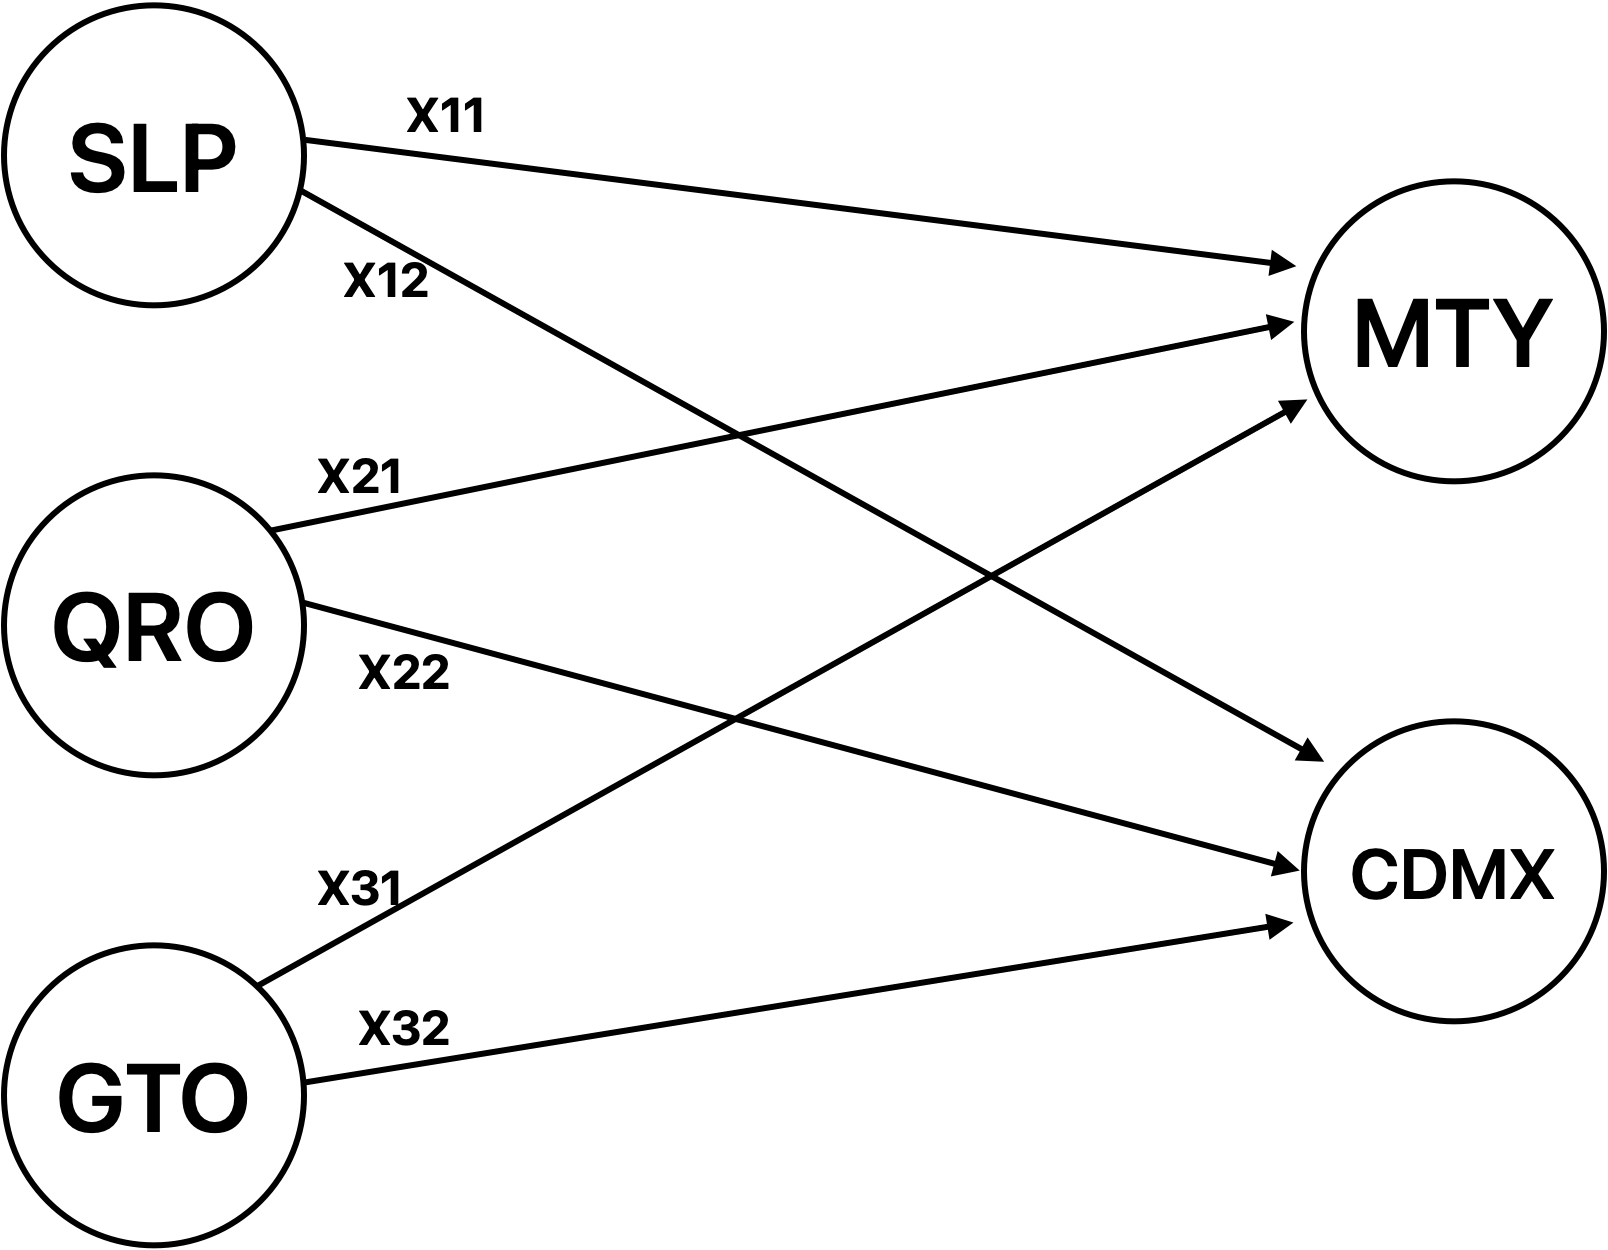
\includegraphics[width=0.8\textwidth]{assets/Prob1GrafImg.png}
\end{figure}

\subsection{Solución con LINGO}
Para resolver problemas de transporte en \textit{LINGO}, comenzamos por definir la función objetivo, que en este caso se trata de minimizar los costos de transporte, los cuales podemos obtener de la Tabla \ref{tab:costoProb1}.
Posteriormente, definimos las restricciones de acuerdo a la oferta, definida en la tabla \ref{tab:oferProb1} y la demanda, definida en la Tabla \ref{tab:demProb1}.
En la figura \ref{fig:lingoProb1} se muestra cómo queda este problema escrito en \textit{LINGO}.

\begin{figure}[H]
	\centering
	\caption{Modelo transporte problema 1 en LINGO}
	\label{fig:lingoProb1}
	\begin{verbatim}
!Funcion objetivo;
min = 80*X11 + 215*X12 + 100*X21 + 180*X22 + 102*X31 + 68*X32;
X11 + X12 = 1000; !Prod SLP;
X21 + X22 = 1500; !Prod QRO;
X31 + X32 = 1200; !Prod GTO;
X11 + X21 + X31 = 2300; !Dem MTY;
X12 + X22 + X32 = 1400; !Dem CDMX;
!Da enteros, no hay medios carros;
	\end{verbatim}
\end{figure}

Notemos, del útimo comentario del modelo un factor importante, que es definir las variables como enteros, pues no podemos entregar fracciones de unidades de nuestro producto, en este caso, no podemos entregar medios carros.\\
Cuando ejecutamos el programa para que nos genere una solución, obtenemos el siguiente reporte:

\begin{figure}[H]
	\centering
	\caption{Reporte resultado LINGO problema 1}
	\label{fig:reporteProb1}
	\begin{verbatim}
  Global optimal solution found.
  Objective value:                              327600.0
  Infeasibilities:                              0.000000
  Total solver iterations:                             1
  Elapsed runtime seconds:                          0.08

  Model Class:                                        LP

  Total variables:                      6
  Nonlinear variables:                  0
  Integer variables:                    0

  Total constraints:                    6
  Nonlinear constraints:                0

  Total nonzeros:                      18
  Nonlinear nonzeros:                   0



                                Variable           Value        Reduced Cost
                                     X11        1000.000            0.000000
                                     X12        0.000000            55.00000
                                     X21        1300.000            0.000000
                                     X22        200.0000            0.000000
                                     X31        0.000000            114.0000
                                     X32        1200.000            0.000000

	\end{verbatim}
\end{figure}

Lo primero que podemos observar del reporte de la figura \ref{fig:reporteProb1} es que el costo total de transportar todas las unidades del producto sería de \$327,600. Después, podemos expresar cuántas unidades se moveran de cada origen a cada destino completando el grafo de la figura \ref{fig:grafoProb1}, obteniendo el grafo de la figura \ref{fig:grafoResProb1}.

\begin{figure}[H]
\centering
\caption{Grafo resuelto para el problema 1.}
\label{fig:grafoResProb1}
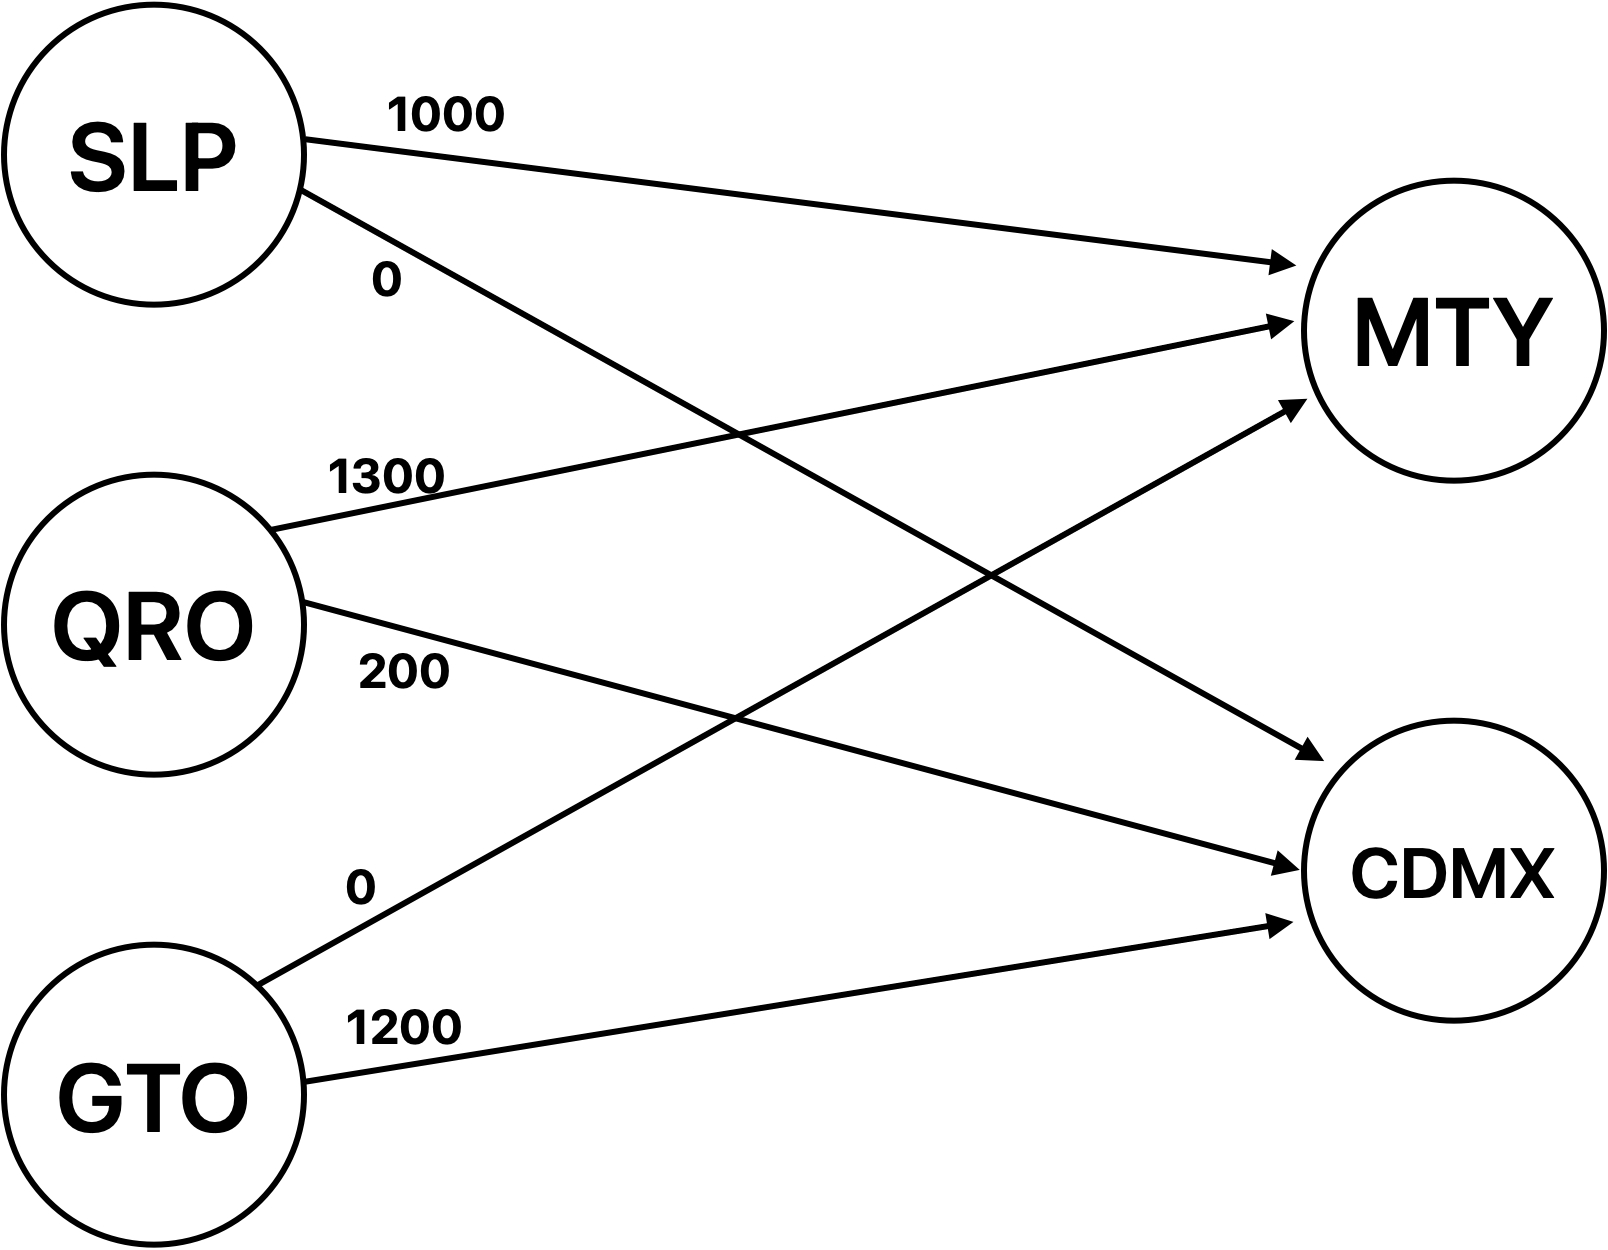
\includegraphics[width=0.8\textwidth]{assets/grafoProb1Res.png}
\end{figure}

En este caso, nos dió desde la primera ejecución una solución con números enteros, sin embargo, en futuros problemas sí que será necesario especificarlo, utilizando la función de LINGO \textbf{@GIN}

\subsection{Solución con Solver}

\section{Modelo de transporte}
Podemos expresar estos problemas de forma más consisa utilizando una sola tabla, en cuyas celdas se muestren los costos de los transporte de cada origen a cada destino y en los extremos de la tabla las ofertas de cada origen (derecha) y la demanda de cada destino (abajo), como se muestra en la tabla \ref{tab:prob2} o bien, utilizando un grafo como el de la figura \ref{fig:grafProb2},donde en cada nodo se indica lo que la fuente (izquierda) oferta y lo que cada destino (derecha) demanda y sobre cada arista se indica el costo de transportar cada unidad de producto de cada origen a cada destino. Hacemos énfasis de nuevo en que para este tipo de porblemas la demanda debe ser equivalente a la oferta.

\begin{table}[H]
\centering
\caption{Costos, oferta y demanda Problema 2}
\label{tab:prob2}
\begin{tabular}{c|ccc|c}
& D1 & D2 & D3 & Oferta $\downarrow$ \\
\hline
F1 & 123 & 254 & 316 & 3600 \\
F2 & 214 & 164 & 323 & 4500 \\
F3 & 364 & 251 & 174 & 2800 \\
\hline
Demanda $\rightarrow$ & 5000 & 2600 & 3300 & 10900/10900
\end{tabular}
\end{table}

\begin{figure}[h]
    \centering
    \caption{Grafo para el Problema 2}
    \label{fig:grafProb2}
    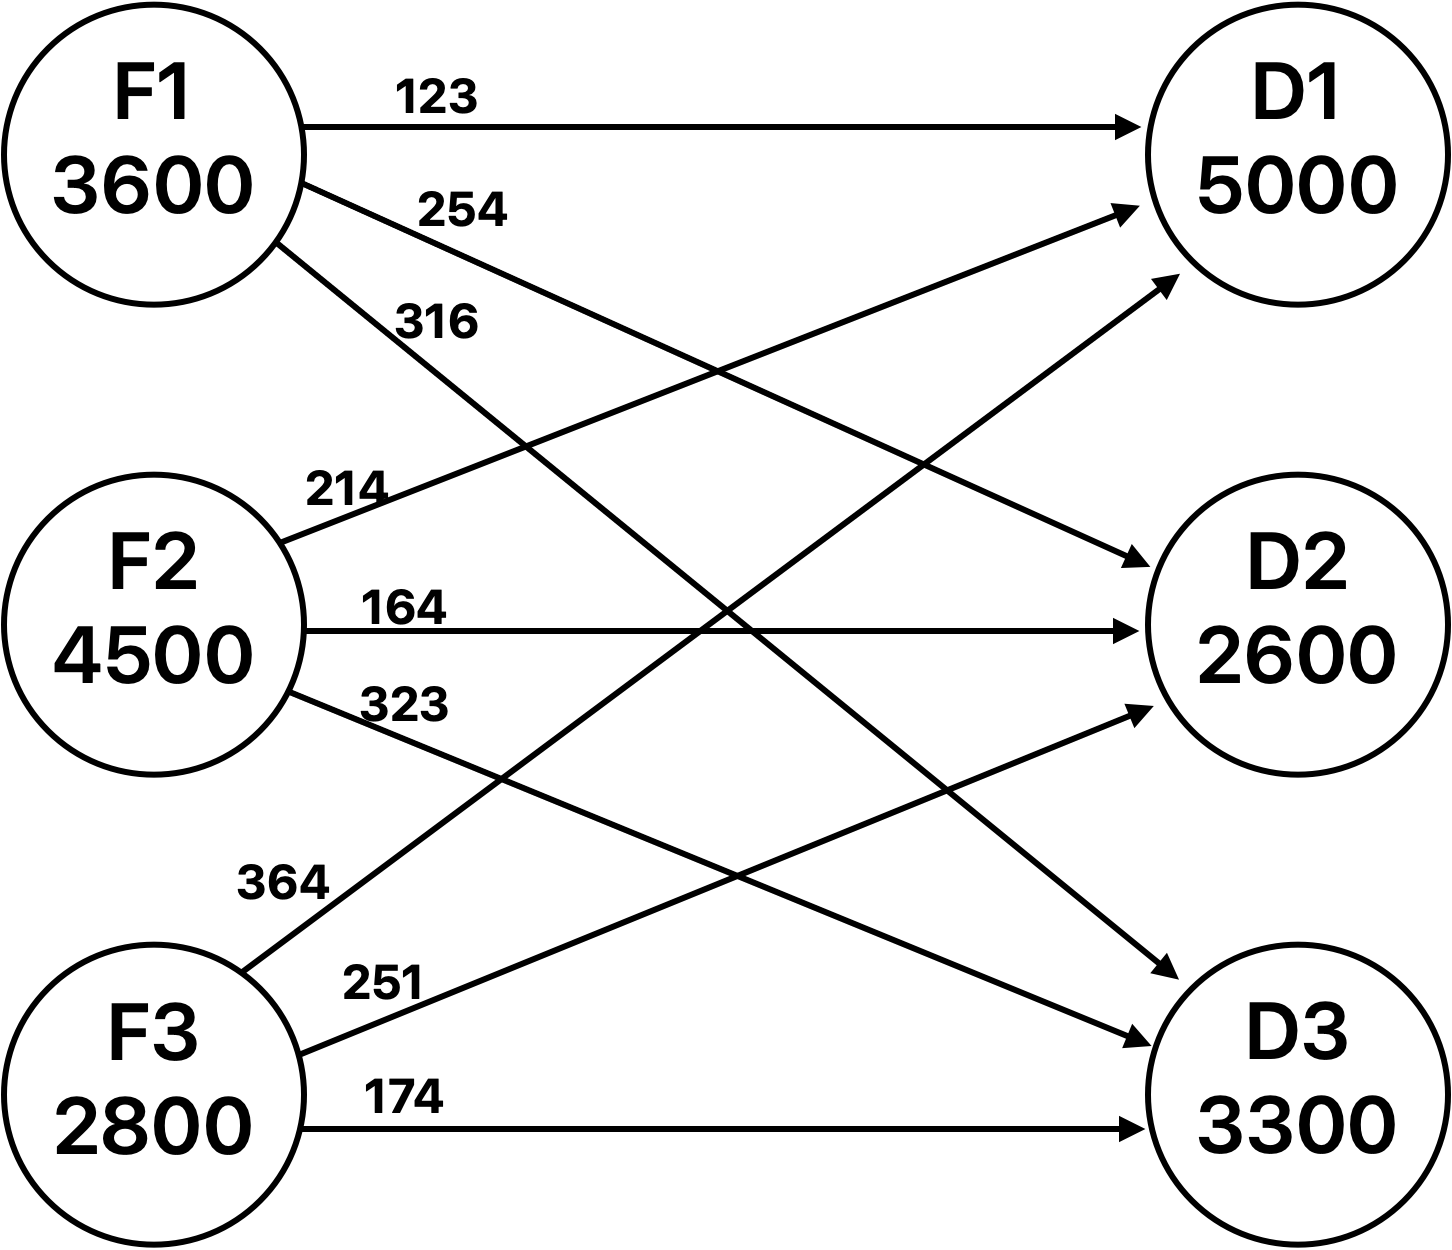
\includegraphics[width=0.8\textwidth]{assets/grafoProb2.png}
\end{figure}

\subsection{Solución con LINGO}
Como en el problema anterior, definimos la función objetivo para reducir los costos de transporte y las restricciones para satisfacer la oferta y la demanda.

\begin{figure}[H]
	\centering
	\caption{Modelo transporte problema 2 en LINGO}
	\label{fig:lingoProb2}
	\begin{verbatim}
!Funcion objetivo;
min = 123*F11 + 254*F12 + 316*F13 + 214*F21 + 164*F22 + 323*F23 + 
364*F31 + 251*F32 + 174*F33;
F11 + F12 + F13 = 3600; !Oferta F1;
F21 + F22 + F23 = 4500; !Oferta F2;
F31 + F32 + F33 = 2800; !Oferta F3;
F11 + F21 + F31 = 5000; !Demanda D1;
F12 + F22 + F32 = 2600; !Demanda D2;
F13 + F23 + F33 = 3300; !Demanda D3;
	\end{verbatim}
\end{figure}

Cuando ejecutamos el modelo de la figura \ref{fig:lingoProb2}, obtenemos el reporte de la figura \ref{fig:reporteProb2}. Vemos que el costo total de trasporte sería de \$1,817,500.

\begin{figure}[H]
	\centering
	\caption{Reporte resultado LINGO problema 2}
	\label{fig:reporteProb2}
	\begin{verbatim}
  Global optimal solution found.
  Objective value:                              1817500.
  Infeasibilities:                              0.000000
  Total solver iterations:                             5
  Elapsed runtime seconds:                          0.04

  Model Class:                                        LP

                                Variable           Value        Reduced Cost
                                     F11        3600.000            0.000000
                                     F12        0.000000            181.0000
                                     F13        0.000000            84.00000
                                     F21        1400.000            0.000000
                                     F22        2600.000            0.000000
                                     F23        500.0000            0.000000
                                     F31        0.000000            299.0000
                                     F32        0.000000            236.0000
                                     F33        2800.000            0.000000
	\end{verbatim}
\end{figure}

Para indicar cuánto producto se mueve de cada origen a cada destino podríamos utilizar un grafo, como se hizo con el problema 1, sin embargo también es posible utilizar una tabla, como en la Tabla \ref{tab:resProb2}

\begin{table}[H]
\centering
\caption{Costos, oferta y demanda Problema 2}
\label{tab:resProb2}
\begin{tabular}{c|ccc}
& D1 & D2 & D3 \\
\hline
F1 & 3600 & 0 & 0 \\
F2 & 1400 & 2600 & 500 \\
F3 & 0 & 0 & 2800 \\
\end{tabular}
\end{table}

\subsection{Solución con Solver}

\section{Transporte: Esquina Noroeste}
Para los dos problemas anteriores, ya analizamos los métodos de LINGO y Solver para su solución. Estudiemos ahora un nuevo método: Esquina Noroeste. Muy parecido a un método visual, comenzamos con una tabla como la Tabla \ref{tab:Prob3}

\begin{table}[H]
\centering
\caption{Tabla inicial Problema 3}
\label{tab:Prob3}
\begin{tabular}{c|ccccc|cc}
& D1 & D2 & D3 & D4 & D5 & Oferta & Restan \\
\hline
S1 &  &  &  &  &  & 250 & 0 \\
S2 &  &  &  &  &  & 250 & 0 \\
S3 &  &  &  &  &  & 250 & 0 \\
S4 &  &  &  &  &  & 250 & 0 \\
\hline
Demanda & 300 & 175 & 325 & 130 & 70 & & \\
Resta & 0 & 0 & 0 & 0 & 0 & & \\
\end{tabular}
\end{table}

Ahora, como lo dice el nombre del método, comenzamos posicionándonos en la esquina nor-oeste de la tabla, es decir la de la esquina superior izquierda y apartir de allí, ejecutamos el algoritmo de la figura \ref{fig:AlgoNoroeste} asignandole a las filas la variable $i$ (inicializada en 1) y a las columnas la variable $j$ (inicializada en 1 también).

\begin{figure}[H]
	\centering
	\caption{Algoritmo Esquina noroeste}
	\label{fig:AlgoNoroeste}
	\begin{enumerate}
		\item Asigna todo lo que puedas de la oferta i a la demanda j
		\item Mientras $i$ y $j$ $< |\text{ofertas}| y |\text{demandas}|$ respectivamente:
		\begin{enumerate}
			\item Si se ha satisfecho la demanda j, pasar a la demanda j+1
			\item Si se a acabado la oferta i, pasar a la oferta i+1
		\end{enumerate}
	\end{enumerate}
\end{figure}

Visto de forma gráfica, la Figura \ref{} muestra la ejecución paso a paso del algoritmo de la esquina nor-oeste para el problema 3.

%O lo haces en Excel o en LaTeX pa. 
\begin{table}[H]
    \centering
        \caption{Paso 1}
        \label{tab:paso1Prob3}
        \begin{tabular}{c|ccccc|cc}
        & D1 & D2 & D3 & D4 & D5 & Oferta & Restan \\
        \hline
        S1 & \cellcolor{yellow} 250 &  &  &  &  & 250 & 0 \\
        S2 &  &  &  &  &  & 250 & 250 \\
        S3 &  &  &  &  &  & 250 & 250 \\
        S4 &  &  &  &  &  & 250 & 250 \\
        \hline
        Demanda & 300 & 175 & 325 & 130 & 70 & & \\
        Resta & 50 & 175 & 325 & 130 & 70 & & \\
        \end{tabular}
\end{table}

\begin{table}[H]
        \centering
        \caption{Paso 2}
        \label{tab:paso2Prob3}
        \begin{tabular}{c|ccccc|cc}
        & D1 & D2 & D3 & D4 & D5 & Oferta & Restan \\
        \hline
        S1 & 250 &  &  &  &  & 250 & 0 \\
        S2 &  \cellcolor{yellow} 50 &  &  &  &  & 250 & 200 \\
        S3 &  &  &  &  &  & 250 & 250 \\
        S4 &  &  &  &  &  & 250 & 250 \\
        \hline
        Demanda & 300 & 175 & 325 & 130 & 70 & & \\
        Resta & 0 & 175 & 325 & 130 & 70 & & \\
        \end{tabular}
\end{table}

\begin{table}[H]
        \centering
        \caption{Paso 3}
        \label{tab:paso3Prob3}
        \begin{tabular}{c|ccccc|cc}
        & D1 & D2 & D3 & D4 & D5 & Oferta & Restan \\
        \hline
        S1 & 250 &  &  &  &  & 250 & 0 \\
        S2 &  50 & \cellcolor{yellow} 175 &  &  &  & 250 & 25 \\
        S3 &  &  &  &  &  & 250 & 250 \\
        S4 &  &  &  &  &  & 250 & 250 \\
        \hline
        Demanda & 300 & 175 & 325 & 130 & 70 & & \\
        Resta & 0 & 0 & 325 & 130 & 70 & & \\
        \end{tabular}
\end{table}

\begin{table}[H]
        \centering
        \caption{Paso 4}
        \label{tab:paso4Prob3}
        \begin{tabular}{c|ccccc|cc}
        & D1 & D2 & D3 & D4 & D5 & Oferta & Restan \\
        \hline
        S1 & 250 &  &  &  &  & 250 & 0 \\
        S2 &  50 & 175 & \cellcolor{yellow} 25 &  &  & 250 & 0 \\
        S3 &  &  &  &  &  & 250 & 250 \\
        S4 &  &  &  &  &  & 250 & 250 \\
        \hline
        Demanda & 300 & 175 & 325 & 130 & 70 & & \\
        Resta & 0 & 0 & 300 & 130 & 70 & & \\
        \end{tabular}
\end{table}

\begin{table}[H]
        \centering
        \caption{Paso 5}
        \label{tab:paso5Prob3}
        \begin{tabular}{c|ccccc|cc}
        & D1 & D2 & D3 & D4 & D5 & Oferta & Restan \\
        \hline
        S1 & 250 &  &  &  &  & 250 & 0 \\
        S2 &  50 & 175 & 25 &  &  & 250 & 0 \\
        S3 &  &  & \cellcolor{yellow} 250 &  &    & 250 & 0 \\
        S4 &  &  &  &  &  & 250 & 250 \\
        \hline
        Demanda & 300 & 175 & 325 & 130 & 70 & & \\
        Resta & 0 & 0 & 50 & 130 & 70 & & \\
        \end{tabular}
\end{table}

\begin{table}[H]
        \centering
        \caption{Paso 6}
        \label{tab:paso6Prob3}
        \begin{tabular}{c|ccccc|cc}
        & D1 & D2 & D3 & D4 & D5 & Oferta & Restan \\
        \hline
        S1 & 250 &  &  &  &  & 250 & 0 \\
        S2 &  50 & 175 & 25 &  &  & 250 & 0 \\
        S3 &  &  & 250 &  &  &  & 0 \\
        S4 &  &  & \cellcolor{yellow} 50 &  &  & 250 & 200 \\
        \hline
        Demanda & 300 & 175 & 325 & 130 & 70 & & \\
        Resta & 0 & 0 & 0 & 130 & 70 & & \\
        \end{tabular}
\end{table}

\begin{table}[H]
        \centering
        \caption{Paso 7}
        \label{tab:paso7Prob3}
        \begin{tabular}{c|ccccc|cc}
        & D1 & D2 & D3 & D4 & D5 & Oferta & Restan \\
        \hline
        S1 & 250 &  &  &  &  & 250 & 0 \\
        S2 &  50 & 175 & 25 &  &  & 250 & 0 \\
        S3 &  &  & 250 &  &  & 250 & 0 \\
        S4 &  &  &  50 & \cellcolor{yellow} 130 &  & 250 & 70 \\
        \hline
        Demanda & 300 & 175 & 325 & 130 & 70 & & \\
        Resta & 0 & 0 & 0 & 0 & 70 & & \\
        \end{tabular}
    \end{table}

\begin{table}[H]
        \centering
        \caption{Paso 8}
        \label{tab:paso8Prob3}
        \begin{tabular}{c|ccccc|cc}
        & D1 & D2 & D3 & D4 & D5 & Oferta & Restan \\
        \hline
        S1 & 250 &  &  &  &  & 250 & 0 \\
        S2 &  50 & 175 & 25 &  &  & 250 & 0 \\
        S3 &  &  & 250 &  &  & 250 & 0 \\
        S4 &  &  &  50 & 130 & \cellcolor{yellow}70 & 250 & 0 \\
        \hline
        Demanda & 300 & 175 & 325 & 130 & 70 & & \\
        Resta & 0 & 0 & 0 & 0 & 0 & & \\
        \end{tabular}
\end{table}

Finalmente obtenemos de forma explícita cuántas unidades se moverán de cada origen a cada destino. Para obtener el costo final, es cuestión de multiplicar cada celda por el costo de transporte por unidad y sumar todo.

Este algoritmo funciona si comenzamos desde cuelquier esquina, pues sería equivalente a una simple reconfiguración del orden de ofertas y demandas. Esa demostración queda como un ejercicio para el lector.

%Ya tocan lso dos de exceso y fuga
\section{Exceso de oferta}
En previos ejemplos se ha hecho énfasis en el requerimiento de que la demanda iguale a la oferta en los problemas de transporte. Sin embargo, si estos problemas están pensados para modelar situaciones del mundo real, es bien probable que esta restricción no siempre se cumpla. Para resolver esta situación, será preciso ajustar nuestro modelo. En los ejemplos que veremos a continuación, esto se logrará generando una fuente o un destino (según corresponda) ficticio que nos ayudará a equilibrar la oferta/demanda.

Resolvamos el sigueinte ejercicio:

\begin{table}[H]
\centering
\caption{Tabla inicial problema 4}
\label{tab:Prob4}
\begin{tabular}{c|cccc|c}
& D1 & D2 & D3 & D4 & Oferta \\
\hline
S1 & 23 & 29 & 23 & 24 & 300 \\
S2 & 25 & 27 & 27 & 28 & 200 \\
S3 & 28 & 34 & 35 & 33 & 200 \\
S4 & 31 & 33 & 37 & 27 & 300 \\
\hline
Dem & 200 & 150 & 300 & 250 & \mbox{1000/900} 
\end{tabular}
\end{table}

En este caso, observamos que la oferta tiene un exceso de 100 unidades con respecto a la demanda. Para solucionar este problema, utilizaremos un procedimiento conocido como \textit{Método Húngaro}.

Este método consiste en crear un destino (u orignen, deoendiendo) \textbf{ficticio} para equilibrar la oferta y la demanda, al cuál le asignaremos un costo de transporte altísimo \textbf{en comparación} con los costos de transporte de los demás nodos del problema.

Para este problema, necesitamos entonces un destino ficticio, con una demanda de 100 y cuyo conste de transporte desde cualquier fuente es de 90, como se muestra en la Tabla \ref{}.

\begin{table}[H]
\centering
\caption{Ajuste con destino ficticio}
\label{tab:ajusteProb4}
\begin{tabular}{c|ccccc|c}
& D1 & D2 & D3 & D4 & DF & Oferta \\
\hline
S1 & 23 & 29 & 23 & 24 & \cellcolor{orange} 90 & 300 \\
S2 & 25 & 27 & 27 & 28 & \cellcolor{orange} 90 & 200 \\
S3 & 28 & 34 & 35 & 33 & \cellcolor{orange} 90 & 200 \\
S4 & 31 & 33 & 37 & 27 & \cellcolor{orange} 90 & 300 \\
\hline
Dem & 200 & 150 & 300 & 250 & \cellcolor{orange} 100 & \mbox{1000/1000} 
\end{tabular}
\end{table}

Una vez equilibrada la oferta con la demanda, podemos aplicar cualquier algoritmo de esquina, procurando dejar el destino ficticio al final, por lo que en este caso, el más conveniente de aplicar será el de la esquina noroeste, cuyo procedimiento se muestra en las tablas \ref{tab:paso1Prob4} a \ref{tab:paso8Prob4}.

\begin{table}[H]
\centering
\caption{Paso 1}
\label{tab:paso1Prob4}
\begin{tabular}{c|ccccc|cc}
%debe haber 7 &ampersands, porque son 8 columnas
& D1 & D2 & D3 & D4 & DF & Oferta & Restan \\
\hline
S1 & \cellcolor{yellow}200 & & & & & 300 & 100 \\
S2 & & & & & & 200 & 200 \\
S3 & & & & & & 200 & 200 \\
S4 & & & & & & 300 & 200 \\
\hline
Dem & 200 & 150 & 300 & 250 & 100 & & \\
Restan & 0 & 150 & 300 & 250 & 100 & & 
\end{tabular}
\end{table}

\begin{table}[H]
\centering
\caption{Paso 2}
\label{tab:paso2Prob4}
\begin{tabular}{c|ccccc|cc}
%debe haber 7 &ampersands, porque son 8 columnas
& D1 & D2 & D3 & D4 & DF & Oferta & Restan \\
\hline
S1 & 200 & \cellcolor{yellow}100 & & & & 300 & 0 \\
S2 & & & & & & 200 & 200 \\
S3 & & & & & & 200 & 200 \\
S4 & & & & & & 300 & 200 \\
\hline
Dem & 200 & 150 & 300 & 250 & 100 & & \\
Restan & 0 & 50 & 300 & 250 & 100 & & 
\end{tabular}
\end{table}

\begin{table}[H]
\centering
\caption{Paso 3}
\label{tab:paso3Prob4}
\begin{tabular}{c|ccccc|cc}
%debe haber 7 &ampersands, porque son 8 columnas
& D1 & D2 & D3 & D4 & DF & Oferta & Restan \\
\hline
S1 & 200 & 100 & & & & 300 & 0 \\
S2 & & \cellcolor{yellow}50 & & & & 200 & 150 \\
S3 & & & & & & 200 & 200 \\
S4 & & & & & & 300 & 200 \\
\hline
Dem & 200 & 150 & 300 & 250 & 100 & & \\
Restan & 0 & 0 & 300 & 250 & 100 & & 
\end{tabular}
\end{table}

\begin{table}[H]
\centering
\caption{Paso 4}
\label{tab:paso4Prob4}
\begin{tabular}{c|ccccc|cc}
%debe haber 7 &ampersands, porque son 8 columnas
& D1 & D2 & D3 & D4 & DF & Oferta & Restan \\
\hline
S1 & 200 & 100 & & & & 300 & 0 \\
S2 & & 50 & \cellcolor{yellow}150 & & & 200 & 0 \\
S3 & & & & & & 200 & 200 \\
S4 & & & & & & 300 & 200 \\
\hline
Dem & 200 & 150 & 300 & 250 & 100 & & \\
Restan & 0 & 0 & 150 & 250 & 100 & & 
\end{tabular}
\end{table}

\begin{table}[H]
\centering
\caption{Paso 5}
\label{tab:paso5Prob4}
\begin{tabular}{c|ccccc|cc}
%debe haber 7 &ampersands, porque son 8 columnas
& D1 & D2 & D3 & D4 & DF & Oferta & Restan \\
\hline
S1 & 200 & 100 & & & & 300 & 0 \\
S2 & & 50 & 150 & & & 200 & 0 \\
S3 & & & \cellcolor{yellow}150 & & & 200 & 50 \\
S4 & & & & & & 300 & 200 \\
\hline
Dem & 200 & 150 & 300 & 250 & 100 & & \\
Restan & 0 & 0 & 0 & 250 & 100 & & 
\end{tabular}
\end{table}

\begin{table}[H]
\centering
\caption{Paso 6}
\label{tab:paso6Prob4}
\begin{tabular}{c|ccccc|cc}
%debe haber 7 &ampersands, porque son 8 columnas
& D1 & D2 & D3 & D4 & DF & Oferta & Restan \\
\hline
S1 & 200 & 100 & & & & 300 & 0 \\
S2 & & 50 & 150 & & & 200 & 0 \\
S3 & & & 150 & \cellcolor{yellow}50 & & 200 & 0 \\
S4 & & & & & & 300 & 200 \\
\hline
Dem & 200 & 150 & 300 & 250 & 100 & & \\
Restan & 0 & 0 & 0 & 200 & 100 & & 
\end{tabular}
\end{table}

\begin{table}[H]
\centering
\caption{Paso 7}
\label{tab:paso7Prob4}
\begin{tabular}{c|ccccc|cc}
%debe haber 7 &ampersands, porque son 8 columnas
& D1 & D2 & D3 & D4 & DF & Oferta & Restan \\
\hline
S1 & 200 & 100 & & & & 300 & 0 \\
S2 & & 50 & 150 & & & 200 & 0 \\
S3 & & & 150 & 50 & & 200 & 0 \\
S4 & & & & \cellcolor{yellow}200 & & 300 & 0 \\
\hline
Dem & 200 & 150 & 300 & 250 & 100 & & \\
Restan & 0 & 0 & 0 & 0 & 100 & & 
\end{tabular}
\end{table}

\begin{table}[H]
\centering
\caption{Paso 8}
\label{tab:paso8Prob4}
\begin{tabular}{c|ccccc|cc}
%debe haber 7 &ampersands, porque son 8 columnas
& D1 & D2 & D3 & D4 & DF & Oferta & Restan \\
\hline
S1 & 200 & 100 & & & & 300 & 0 \\
S2 & & 50 & 150 & & & 200 & 0 \\
S3 & & & 150 & 50 & & 200 & 0 \\
S4 & & & & 200 & \cellcolor{yellow}100 & 300 & 0 \\
\hline
Dem & 200 & 150 & 300 & 250 & 100 & & \\
Restan & 0 & 0 & 0 & 0 & 0 & & 
\end{tabular}
\end{table}

Con el algoritmo terminado, multiplicamos el número de unidades transportadas de cada origen a cada destino por el costo individual correspondiente, para obtener un subtotal o total previo. En este caso, la operación desglosada sería

\begin{align*}
(200 \times 23) + (100 \times 29) + (50 \times 27) + (150 \times 27) + (150 \times 35) \\
+ (50 \times 33) + (200 \times 27) + (100 \times 90) = 34200
\end{align*}

A este total previo, debemos restarle lo correspondiente al transporte hacia el destino ficticio, en este caso sería

\begin{align}
34200 - (100 \times 90) \\ 
34200 - 9000 = 25200
\end{align}

Obtenemos de esta forma, el costo total real para la solución óptima de este problema, que es de \$25,200.

\subsection{LINGO}
Podemos modelar este problema en LINGO, tanto como para ver cómo se modelan este tipo de problemas, como para comparar las respuestas que obtenemos.

En solver, este problema se vería expresado de la siguiente forma:

\begin{figure}[H]
	\centering
	\caption{Modelo transporte problema 4 en LINGO}
	\label{fig:lingoProb4}
	\begin{verbatim}
!Funcion objetivo;
!Primero el D y luego el S;
min = 23*D1S1 + 29*D2S1 + 23*D3S1 + 24*D4S1 + 90*DFS1
+ 25*D1S2 + 27*D2S2 + 27*D3S2 + 28*D4S2 + 90*DFS2
+ 28*D1S3 + 34*D2S3 + 35*D3S3 + 33*D4S3 + 90*DFS3
+ 31*D1S4 + 33*D2S4 + 37*D3S4 + 27*D4S4 + 90*DFS4;
!Restricciones;
!Demanda;
D1S1 + D1S2 + D1S3 + D1S4 = 200;
D2S1 + D2S2 + D2S3 + D2S4 = 150;
D3S1 + D3S2 + D3S3 + D3S4 = 300;
D4S1 + D4S2 + D4S3 + D4S4 = 250;
DFS1 + DFS2 + DFS3 + DFS4 = 100;
!Oferta;
D1S1 + D2S1 + D3S1 + D4S1 + DFS1 = 300;
D1S2 + D2S2 + D3S2 + D4S2 + DFS2 = 200;
D1S3 + D2S3 + D3S3 + D4S3 + DFS3 = 200;
D1S4 + D2S4 + D3S4 + D4S4 + DFS4 = 300;
	\end{verbatim}
\end{figure}

Cuando ejecutamos el modelo de la figura \ref{fig:lingoProb4}, obtenemos el reporte de la figura \ref{fig:reporteProb4}. Vemos que el costo total previo de trasporte sería de \$32,150 precio al que debemos restarle lo asignado al destino ficticio 

\begin{align}
32150 - (50 \times 2 \times 90) \\ 
32150 - 9000 = 23150
\end{align}

Lo que de entrada es menos que el costo total previo obtenido con el algoritmo de la esquina noroeste.
Analicemos entonces el movimiento de las unidades.

\begin{figure}[H]
	\centering
	\caption{Reporte resultado LINGO problema 4}
	\label{fig:reporteProb4}
	\begin{verbatim}
  Global optimal solution found.
  Objective value:                              32150.00
  Infeasibilities:                              0.000000
  Total solver iterations:                             8
  Elapsed runtime seconds:                          0.08

  Model Class:                                        LP

  Total variables:                     20

                                Variable           Value        Reduced Cost
                                    D1S1        0.000000            0.000000
                                    D2S1        0.000000            4.000000
                                    D3S1        300.0000            0.000000
                                    D4S1        0.000000            2.000000
                                    DFS1        0.000000            5.000000
                                    D1S2        50.00000            0.000000
                                    D2S2        150.0000            0.000000
                                    D3S2        0.000000            2.000000
                                    D4S2        0.000000            4.000000
                                    DFS2        0.000000            3.000000
                                    D1S3        150.0000            0.000000
                                    D2S3        0.000000            4.000000
                                    D3S3        0.000000            7.000000
                                    D4S3        0.000000            6.000000
                                    DFS3        50.00000            0.000000
                                    D1S4        0.000000            3.000000
                                    D2S4        0.000000            3.000000
                                    D3S4        0.000000            9.000000
                                    D4S4        250.0000            0.000000
                                    DFS4        50.00000            0.000000
	\end{verbatim}
\end{figure}

%Continúa aquí el análisis
%YA SÉ! Hace falta restarle lo del destino ficticio a lo de LINGO PTM

Si comparamos lado a lado la tabla \ref{tab:esqNorEstProb4} obtenida del algoritmo de esquina noroeste con el reporte de LINGO, expresado en la tabla \ref{tab:solLingoProb4} observamos que ambas satisfacen correctamente los requerimientos de oferta y demanda; sin embargo, la distribución de los recursos en la solución de LINGO difiere de la escalonada obtenida con el agloritmo de la esquina noroeste.

Esta diferencia de distribución y consecuentemente de precio seguramente se deba a la diferencia de métodos utilizados para llegar a la solución, específicamente al método \textbf{Simplex} utilizado por LINGO, que garantiza el precio mínimo matemáticamente posible.

\begin{table}[H]
\centering
\caption{Esquina noroeste Problema 4}
\label{tab:esqNorEstProb4}
\begin{tabular}{c|ccccc|cc}
%debe haber 7 &ampersands, porque son 8 columnas
& D1 & D2 & D3 & D4 & DF & Oferta & Restan \\
\hline
S1 & 200 & 100 & & & & 300 & 0 \\
S2 & & 50 & 150 & & & 200 & 0 \\
S3 & & & 150 & 50 & & 200 & 0 \\
S4 & & & & 200 & 100 & 300 & 0 \\
\hline
Dem & 200 & 150 & 300 & 250 & 100 & & \\
Restan & 0 & 0 & 0 & 0 & 0 & & 
\end{tabular}
\end{table}

\begin{table}[H]
\centering
\caption{Solución LINGO Problema 4}
\label{tab:solLingoProb4}
\begin{tabular}{c|ccccc|cc}
%debe haber 7 &ampersands, porque son 8 columnas
& D1 & D2 & D3 & D4 & DF & Oferta & Restan \\
\hline
S1 & & & 300 & & & 300 & 0 \\
S2 & 50 & 150 & & & & 200 & 0 \\
S3 & 150 & & & & 50 & 200 & 0 \\
S4 & & & & 250 & 50 & 300 & 0 \\
\hline
Dem & 200 & 150 & 300 & 250 & 100 & & \\
Restan & 0 & 0 & 0 & 0 & 0 & & 
\end{tabular}
\end{table}

\section{Exceso de demanda}
Por supuesto que el problema de desigualdad también puede darse en la demanda. Resolvamos el siguiente problema:

\begin{table}[H]
\centering
\caption{Tabla inicial problema 5}
\label{tab:Prob5}
\begin{tabular}{c|ccccc|c}
& D1 & D2 & D3 & D4 & D5 & Oferta \\
\hline
S1 & 145 & 154 & 169 & 171 & 142 & 3000 \\
S2 & 165 & 167 & 144 & 143 & 161 & 4500 \\
S3 & 178 & 148 & 158 & 156 & 153 & 3000 \\
\hline
Dem & 1200 & 2000 & 2500 & 3500 & 2000 & \mbox{10500/11200} 
\end{tabular}
\end{table}

Las técnicas en este caso son las mismas que en el problema anterior. Comenzamos por definir un orignen ficticio $S4$ con la oferta suficiente para equilibrar la demanda y cuyos costos de transporte sean bastante elevados en comparación con el resto de costos de transporte del problema.

\begin{table}[H]
\centering
\caption{Tabla inicial problema 5}
\label{tab:ajusteProb5}
\begin{tabular}{c|ccccc|c}
& D1 & D2 & D3 & D4 & D5 & Oferta \\
\hline
S1 & 145 & 154 & 169 & 171 & 142 & 3000 \\
S2 & 165 & 167 & 144 & 143 & 161 & 4500 \\
S3 & 178 & 148 & 158 & 156 & 153 & 3000 \\
S4 & 400 & 400 & 400 & 400 & 400 & 700 \\
\hline
Dem & 1200 & 2000 & 2500 & 3500 & 2000 & \mbox{11200/11200} 
\end{tabular}
\end{table}

Resolvamos primero, como lo hicimos anteriormente, con el método de la esquina noroeste.

\begin{table}[H]
\centering
\caption{Paso 1}
\label{tab:Paso1Prob5}
\begin{tabular}{c|ccccc|cc}
& D1 & D2 & D3 & D4 & D5 & Oferta & Restan\\
\hline
S1 & \cellcolor{yellow}1200 &  &  &  &  & 3000 & 1800 \\
S2 &  &  &  &  &  & 4500 & 4500 \\
S3 &  &  &  &  &  & 3000 & 3000 \\
S4 &  &  &  &  &  & 700 & 700 \\
\hline
Demanda & 1200 & 2000 & 2500 & 3500 & 2000 & & \\
Restan & 0 & 2000 & 2500 & 3500 & 2000 &&
\end{tabular}
\end{table}

\begin{table}[H]
\centering
\caption{Paso 2}
\label{tab:Paso2Prob5}
\begin{tabular}{c|ccccc|cc}
& D1 & D2 & D3 & D4 & D5 & Oferta & Restan\\
\hline
S1 & 1200 & \cellcolor{yellow}1800 &  &  &  & 3000 & 0 \\
S2 &  &  &  &  &  & 4500 & 4500 \\
S3 &  &  &  &  &  & 3000 & 3000 \\
S4 &  &  &  &  &  & 700 & 700 \\
\hline
Demanda & 1200 & 2000 & 2500 & 3500 & 2000 && \\
Restan & 0 & 200 & 2500 & 3500 & 2000 &&
\end{tabular}
\end{table}

\begin{table}[H]
\centering
\caption{Paso 3}
\label{tab:Paso3Prob5}
\begin{tabular}{c|ccccc|cc}
& D1 & D2 & D3 & D4 & D5 & Oferta & Restan\\
\hline
S1 & 1200 & 1800 &  &  &  & 3000 & 0 \\
S2 &  & \cellcolor{yellow}200 &  &  &  & 4500 & 4300 \\
S3 &  &  &  &  &  & 3000 & 3000 \\
S4 &  &  &  &  &  & 700 &700 \\
\hline
Demanda & 1200 & 2000 & 2500 & 3500 & 2000 & & \\
Restan & 0 & 0 & 2500 & 3500 & 2000 &&
\end{tabular}
\end{table}

\begin{table}[H]
\centering
\caption{Paso 4}
\label{tab:Paso4Prob5}
\begin{tabular}{c|ccccc|cc}
& D1 & D2 & D3 & D4 & D5 & Oferta & Restan\\
\hline
S1 & 1200 & 1800 &  &  &  & 3000 & 0 \\
S2 &  & 200 & \cellcolor{yellow}2500 &  &  & 4500 & 1800 \\
S3 &  &  &  &  &  & 3000 & 3000 \\
S4 &  &  &  &  &  & 700 &700 \\
\hline
Demanda & 1200 & 2000 & 2500 & 3500 & 2000 & & \\
Restan & 0 & 0 & 0 & 3500 & 2000 &&
\end{tabular}
\end{table}

\begin{table}[H]
\centering
\caption{Paso 5}
\label{tab:Paso5Prob5}
\begin{tabular}{c|ccccc|cc}
& D1 & D2 & D3 & D4 & D5 & Oferta & Restan\\
\hline
S1 & 1200 & 1800 &  &  &  & 3000 & 0 \\
S2 &  & 200 & 2500 & \cellcolor{yellow}1800 &  & 4500 & 0 \\
S3 &  &  &  &  &  & 3000 & 3000 \\
S4 &  &  &  &  &  & 700 &700 \\
\hline
Demanda & 1200 & 2000 & 2500 & 3500 & 2000 & & \\
Restan & 0 & 0 & 0 & 1700 & 2000 &&
\end{tabular}
\end{table}

\begin{table}[H]
\centering
\caption{Paso 6}
\label{tab:Paso6Prob5}
\begin{tabular}{c|ccccc|cc}
& D1 & D2 & D3 & D4 & D5 & Oferta & Restan\\
\hline
S1 & 1200 & 1800 &  &  &  & 3000 & 0 \\
S2 &  & 200 & 2500 & 1800 &  & 4500 & 0 \\
S3 &  &  &  & \cellcolor{yellow}1700 &  & 3000 & 1300 \\
S4 &  &  &  &  &  & 700 &700 \\
\hline
Demanda & 1200 & 2000 & 2500 & 3500 & 2000 & & \\
Restan & 0 & 0 & 0 & 0 & 2000 &&
\end{tabular}
\end{table}

\begin{table}[H]
\centering
\caption{Paso 7}
\label{tab:Paso7Prob5}
\begin{tabular}{c|ccccc|cc}
& D1 & D2 & D3 & D4 & D5 & Oferta & Restan\\
\hline
S1 & 1200 & 1800 &  &  &  & 3000 & 0 \\
S2 &  & 200 & 2500 & 1800 &  & 4500 & 0 \\
S3 &  &  &  & 1700 & \cellcolor{yellow}1300 & 3000 & 0 \\
S4 &  &  &  &  &  & 700 &700 \\
\hline
Demanda & 1200 & 2000 & 2500 & 3500 & 2000 & & \\
Restan & 0 & 0 & 0 & 0 & 700 &&
\end{tabular}
\end{table}

\begin{table}[H]
\centering
\caption{Paso 8}
\label{tab:Paso8Prob5}
\begin{tabular}{c|ccccc|cc}
& D1 & D2 & D3 & D4 & D5 & Oferta & Restan\\
\hline
S1 & 1200 & 1800 &  &  &  & 3000 & 0 \\
S2 &  & 200 & 2500 & 1800 &  & 4500 & 0 \\
S3 &  &  &  & 1700 & 1300 & 3000 & 0 \\
S4 &  &  &  &  & \cellcolor{yellow}700 & 700 &0 \\
\hline
Demanda & 1200 & 2000 & 2500 & 3500 & 2000 & & \\
Restan & 0 & 0 & 0 & 0 & 0 &&
\end{tabular}
\end{table}

Con el algoritmo terminado, multiplicamos el número de unidades transportadas de cada origen a cada destino por el costo individual correspondiente, para obtener un subtotal o total previo. En este caso, la operación desglosada sería

\begin{align*}
(1200 \times 145) + (1800 \times 154) + (200 \times 167) + (2500 \times 144) + (1800 \times 143) \\
+ (1700 \times 156) + (1300 \times 153) + (700 \times 400) = 1,846,100
\end{align*}

A este total previo, debemos restarle lo correspondiente al transporte desde el origen ficticio, en este caso sería

\begin{align}
1846100 - (700 \times 400) \\ 
1846100 - 280000 = 1566100
\end{align}

Obtenemos de esta forma, el costo total real para la solución óptima de este problema, que es de \$1,566,100.

\subsection{LINGO}
Podemos modelar este problema en Solver para comparar las respuestas que obtenemos.

En solver, este problema se vería expresado de la siguiente forma:

\begin{figure}[H]
	\centering
	\caption{Modelo transporte problema 5 en LINGO}
	\label{fig:lingoProb5}
	\begin{verbatim}
!Funcion objetivo;
!Primero el D y luego el S;
min = 145*D1S1 + 154*D2S1 + 169*D3S1 + 171*D4S1 + 142*D5S1
+ 165*D1S2 + 167*D2S2 + 144*D3S2 + 143*D4S2 + 161*D5S2
+ 178*D1S3 + 148*D2S3 + 158*D3S3 + 156*D4S3 + 153*D5S3
+ 400*D1S4 + 400*D2S4 + 400*D3S4 + 400*D4S4 + 400*D5S4;
!Restricciones;
!Demanda;
D1S1 + D1S2 + D1S3 + D1S4 = 1200;
D2S1 + D2S2 + D2S3 + D2S4 = 2000;
D3S1 + D3S2 + D3S3 + D3S4 = 2500;
D4S1 + D4S2 + D4S3 + D4S4 = 3500;
D5S1 + D5S2 + D5S3 + D5S4 = 2000;
!Oferta;
D1S1 + D2S1 + D3S1 + D4S1 + D5S1 = 3000;
D1S2 + D2S2 + D3S2 + D4S2 + D5S2 = 4500;
D1S3 + D2S3 + D3S3 + D4S3 + D5S3 = 3000;
D1S4 + D2S4 + D3S4 + D4S4 + D5S4 = 700;
	\end{verbatim}
\end{figure}

Cuando ejecutamos el modelo de la figura \ref{fig:lingoProb5}, obtenemos el reporte de la figura \ref{fig:reporteProb5}. Vemos que el costo total previo de trasporte sería de \$1,806,300 precio al que debemos restarle lo asignado al destino ficticio 

\begin{align}
1806300 - (700 \times 400) \\ 
1806300 - 280000 = 1783150
\end{align}

\begin{figure}[H]
	\centering
	\caption{Reporte resultado LINGO problema 5}
	\label{fig:reporteProb5}
	\begin{verbatim}
	  Global optimal solution found.
  Objective value:                              1806300.
  Infeasibilities:                              0.000000
  Total solver iterations:                             8
  Elapsed runtime seconds:                          0.07

  Model Class:                                        LP

                                Variable           Value        Reduced Cost
                                    D1S1        1200.000            0.000000
                                    D2S1        0.000000            17.00000
                                    D3S1        0.000000            23.00000
                                    D4S1        0.000000            26.00000
                                    D5S1        1800.000            0.000000
                                    D1S2        0.000000            22.00000
                                    D2S2        0.000000            32.00000
                                    D3S2        1800.000            0.000000
                                    D4S2        2700.000            0.000000
                                    D5S2        0.000000            21.00000
                                    D1S3        0.000000            22.00000
                                    D2S3        2000.000            0.000000
                                    D3S3        0.000000            1.000000
                                    D4S3        800.0000            0.000000
                                    D5S3        200.0000            0.000000
                                    D1S4        0.000000            1.000000
                                    D2S4        0.000000            9.000000
                                    D3S4        700.0000            0.000000
                                    D4S4        0.000000            1.000000
                                    D5S4        0.000000            4.000000
	\end{verbatim}
\end{figure}

Como en el problema anterior, comparemos lado a lado las tablas de transporte y precios obtenidos por ambos procedimientos. En la tabla \ref{tab:esqNorEstProb5} el de la esquina noroeste, con un costo total de \$1,566,100 y en la tabla \ref{tab:solLingoProb5} la solución de LINGO, con un costo total de \$1,783,150.

\begin{table}[H]
\centering
\caption{Esquina noroeste Problema 5}
\label{tab:esqNorEstProb5}
\begin{tabular}{c|ccccc|cc}
& D1 & D2 & D3 & D4 & D5 & Oferta & Restan\\
\hline
S1 & 1200 & 1800 &  &  &  & 3000 & 0 \\
S2 &  & 200 & 2500 & 1800 &  & 4500 & 0 \\
S3 &  &  &  & 1700 & 1300 & 3000 & 0 \\
S4 &  &  &  &  & 700 & 700 &0 \\
\hline
Demanda & 1200 & 2000 & 2500 & 3500 & 2000 & & \\
Restan & 0 & 0 & 0 & 0 & 0 &&
\end{tabular}
\end{table}

\begin{table}[H]
\centering
\caption{Solución LINGO Problema 5}
\label{tab:solLingoProb5}
\begin{tabular}{c|ccccc|cc}
& D1 & D2 & D3 & D4 & D5 & Oferta & Restan\\
\hline
S1 & 1200 & 1800 &  &  & 1800 & 3000 & 0 \\
S2 &  &  & 1800 & 2700 &  & 4500 & 0 \\
S3 &  & 2000 &  & 800 & 200 & 3000 & 0 \\
S4 &  &  & 700 &  &  & 700 &0 \\
\hline
Demanda & 1200 & 2000 & 2500 & 3500 & 2000 & & \\
Restan & 0 & 0 & 0 & 0 & 0 &&
\end{tabular}
\end{table}

Curiosamente, esta vez el resultado fue diferente al problema anterior, y fue el método de la esquina noroeste el que nos entregó un costo total menor en comparación con el método Simplex de LINGO.

Como conslusión de estas últimas observaciones comparando resultado, lo recomendable es revisar con los métodos disponibles en función del tiempo de análisis del que se disponga y comparar resultados para escoger el más óptimo.

Además, como indicó el Profesor Rito en clase, a las personas a quienes se les suelen presentar las soluciones de estos modelos les es preferible que se les muestren diversas opciones para que puedan elegir (ingeiería social, supongo).

\section{Transbordo}
El modelo de transbordo es una clase de programación lineal que tiene que ver con transportar un artículo desde sus fuentes (fábricas), pasando por un transbordo (bodega, reposo, recarga), hasta su destino (distribuidor, cliente).

\textbf{Ejemplo:} Cisterna de leche sale de Monterrey durante la noche, al salir el sol, se encierra en una bodega en queretaro, y durante la noche continúa su trayecto hacia CDMX.

El objetivo es determinar un programa de transporte que minimalice el costo total del transporte y transbordo y que al mismo tiempo satisfaga los límites de oferta y demanda.

En el modelo se supone que el costo de transporte es proporcional a la cantidad de unidades transportadas en determinada ruta, el transbordo indica un segundo costo de transporte, no de almacenamiento.

El problema general se representa en una red, hay $x$ fuentes, $y$ transbordos y $z$ destinos, cada fuente, transbordo y destino se representa con un nodo.

Las rutas que enlazan las fuentes, transbordos y destinos se representan con aristas.

Cada arco une a la fuente $i$ con el transbordo $j$, y cada transbordo $j$ con el destino $k$, conllevando dos datos importantes: el costo de transportar una unidad, y la cantidad transportada.

La cantidad de artículos ofertados desde las fuentes es la demanda por los destinos \mbox{oferta = demanda}.

Resolvamos entonces el siguiente problema, expresando en un grafo en la Figura \ref{fig:grafProb6}, los pesos de las tablas, esta vez, se colocaron en la Tabla \ref{tab:PesosProb6}:

\begin{figure}[h]
    \centering
    \caption{Grafo para el Problema 6}
    \label{fig:grafProb6}
    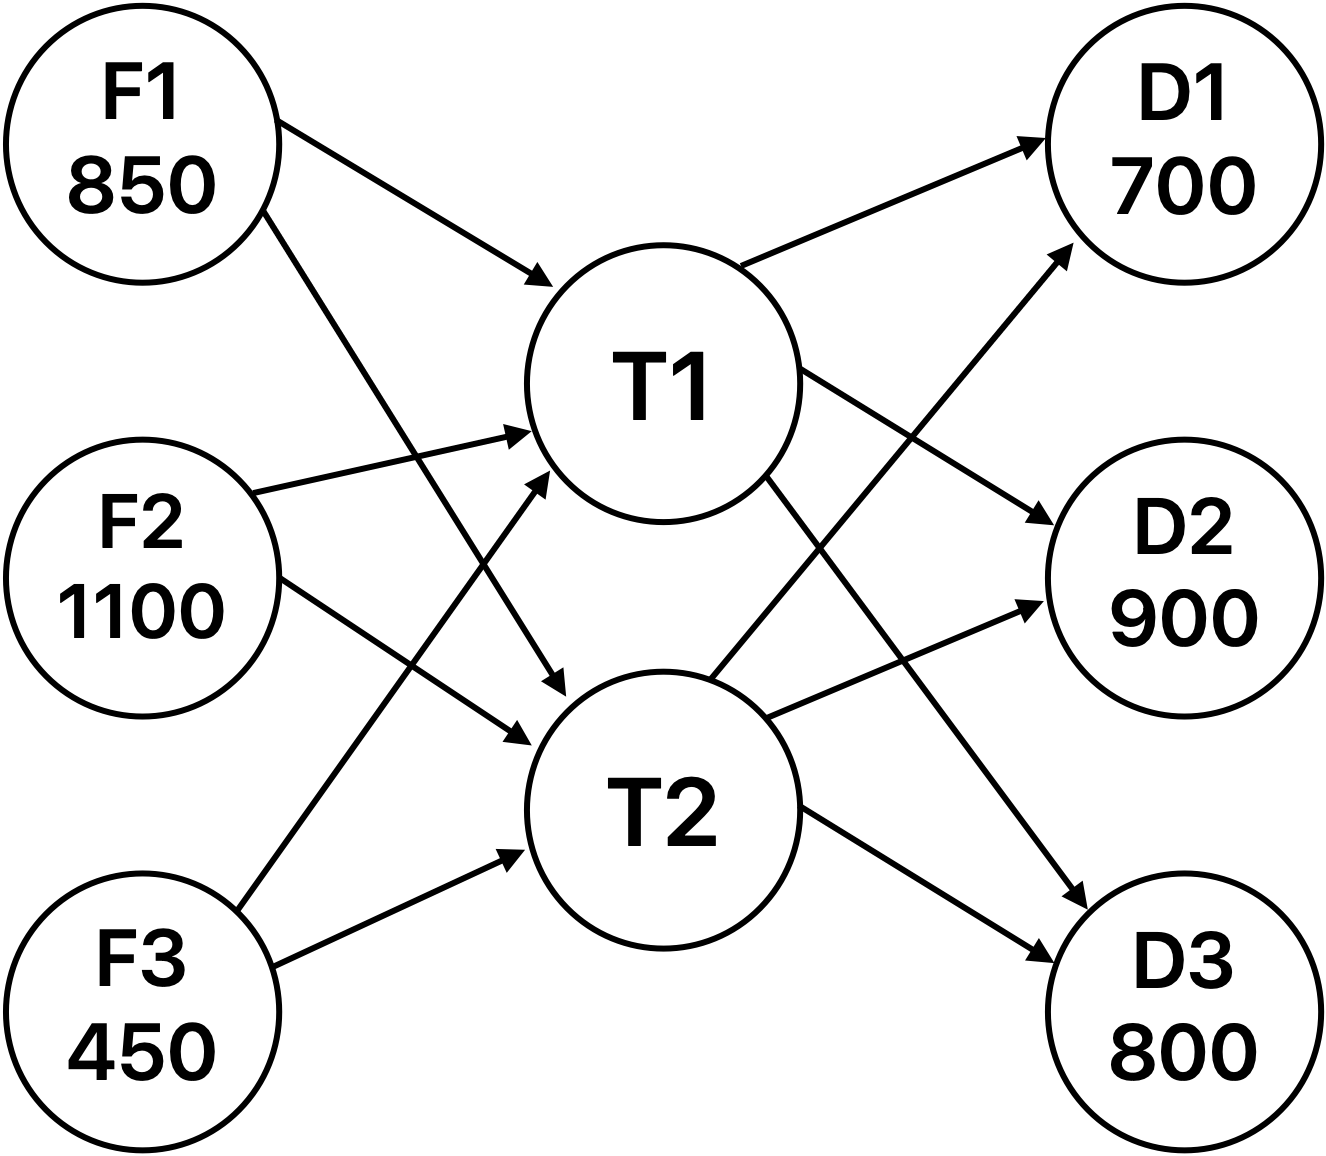
\includegraphics[width=0.8\textwidth]{assets/grafoProb6.png}
\end{figure}

\begin{table}[H]
\centering
\caption{Pesos de aristas grafo Problema 6}
\label{tab:PesosProb6}
\begin{tabular}{lr}
x11 & 8 \\
x12 & 6 \\
x21 & 5 \\
x22 & 7 \\
x31 & 9 \\
x32 & 11 \\
x41 & 14 \\
x42 & 17 \\
x43 & 13 \\
x51 & 16 \\
x52 & 18 \\
x53 & 21
\end{tabular}
\end{table}

\subsection{LINGO}
Para expresar este modelo en LINGO y poder buscar una solución, definimos la función objetivo en función de los costos de transporte individuales expresados en la Tabla \ref{tab:PesosProb6} y especificamos que buscamos minimizarla.

Posteriormente, para las restricciones, colocamos la oferta de cada fuente y la demanda de cada destino, como lo hemos hecho en los problemas anteriores. Lo particular de este problema son los nodos intermedios de transbordo, en estos, dado que nada se almacena, lo que entra desde las fuentes (positivo) debe salir hacia los destinos (negativo), dando un balance total de cero. Observemos entonces el modelo en a Figura \ref{fig:lingoProb6}

\begin{figure}[H]
	\centering
	\caption{Modelo transbordo problema 6 en LINGO}
	\label{fig:lingoProb6}
	\begin{verbatim}
!Costos transporte, funcion objetivo;
min = 8*X11 + 6*X12 + 5*X21 + 7*X22 + 9*X31 + 11*X32 +
14*X41 + 17*X42 + 13*X43 + 16*X51 + 18*X52 + 21*X53;
!Restriciones;

!Fuentes;
X11 + X12 = 850;
X21 + X22 = 1100;
X31 + X32 = 450;

!Transordo;
X11 + X21 + X31 - X41 - X42 - X43 = 0;
X12 + X22 + X32 - X51 - X52 - X53 = 0;

!Destino;
X41 + X51 = 700;
X42 + X52 = 900;
X43 + X53 = 800;
	\end{verbatim}
\end{figure}

Cuando ejecutamos el modelo para obtener una solución, obtenemos el reporte de la Figura \ref{fig:reporteProb6}, obteniendo un costo total de \$51,000.

\begin{figure}[H]
	\centering
	\caption{Reporte resultado LINGO problema 6}
	\label{fig:reporteProb6}
	\begin{verbatim}
  Global optimal solution found.
  Objective value:                              51000.00
  Infeasibilities:                              0.000000
  Total solver iterations:                             1
  Elapsed runtime seconds:                          0.06

  Model Class:                                        LP

                                Variable           Value        Reduced Cost
                                     X11        0.000000            1.000000
                                     X12        850.0000            0.000000
                                     X21        1100.000            0.000000
                                     X22        0.000000            3.000000
                                     X31        450.0000            0.000000
                                     X32        0.000000            3.000000
                                     X41        700.0000            0.000000
                                     X42        50.00000            0.000000
                                     X43        800.0000            0.000000
                                     X51        0.000000            1.000000
                                     X52        850.0000            0.000000
                                     X53        0.000000            7.000000
	\end{verbatim}
\end{figure}

Esta solución puede expresarse en la figura \ref{fig:resProb6} sobre el grafo inicial indicando sobre cada arista las unidades a transportar entre nodos.

\begin{figure}[h]
    \centering
    \caption{Grafo solución para el Problema 6}
    \label{fig:resProb6}
    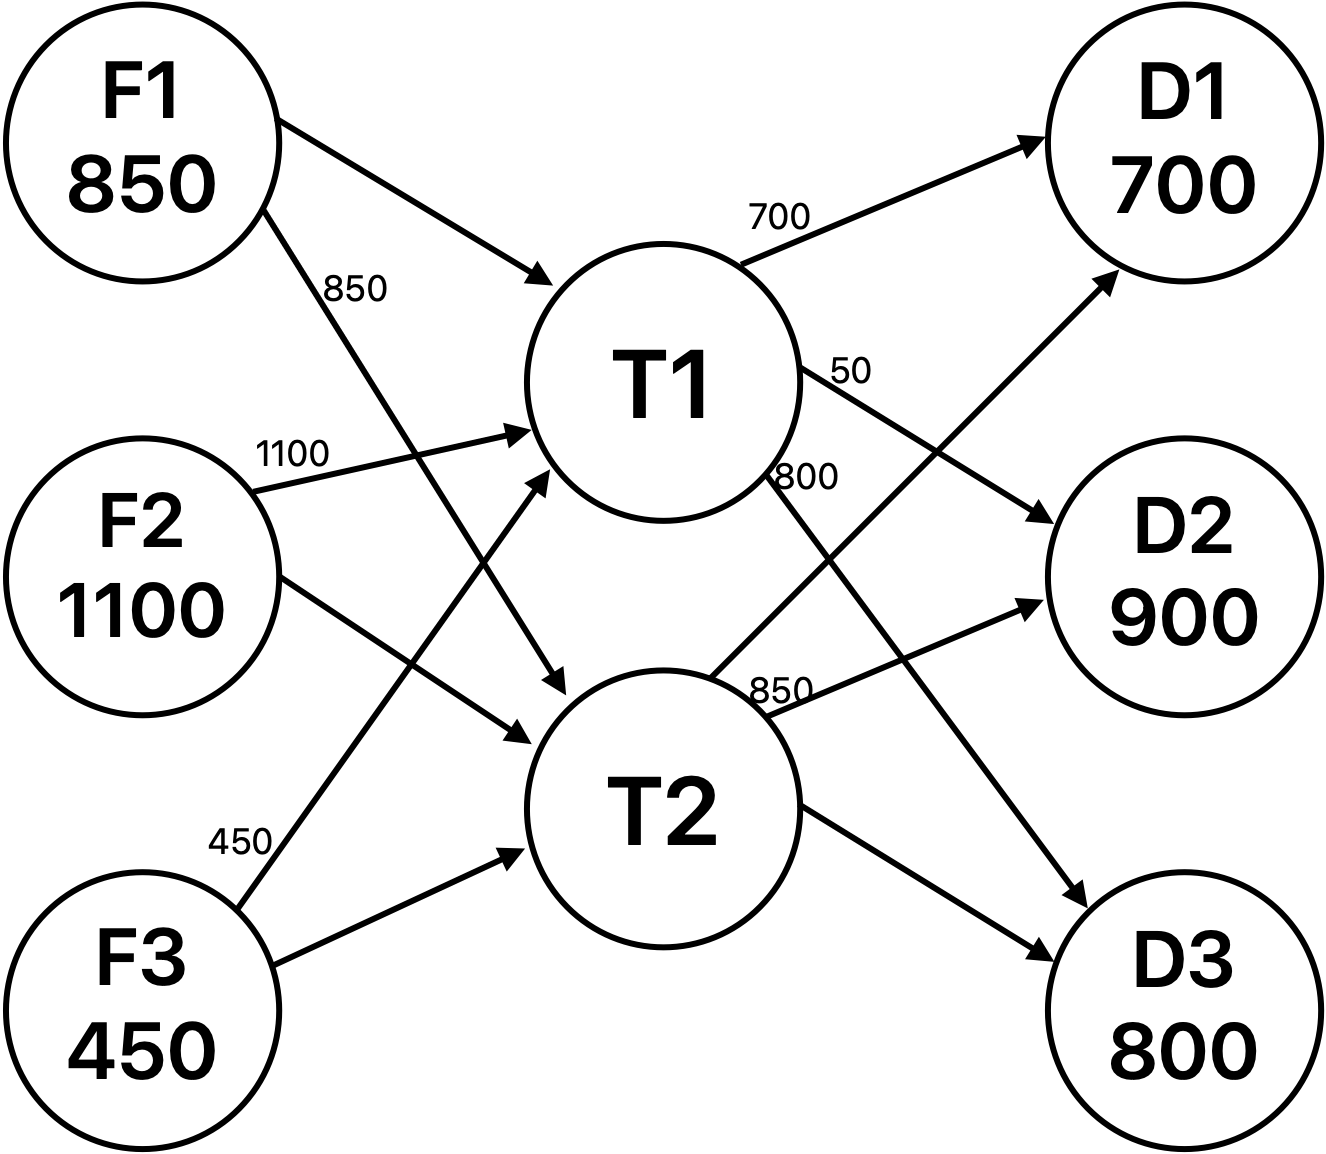
\includegraphics[width=0.8\textwidth]{assets/GrafoSolProb6.png}
\end{figure}

\subsection{Solver}
Para resolver problemas de transbordo en solver, basémonos en el grafo de la figura \ref{fig:grafoProb7}. Para esto, haremos uso de un estilo de tablas como el de la figura \ref{fig:solverProb6}, en el que los costos de cada arista se expresan en la tabla superior, las ofertas, transbordos y demandas en la tabla central y en la tabla inferior indicamos la dirección de las aristas entre los nodos con un 1 si es entrada y un -1 si es salida. En esta última tabla, utilizamos la función SUMPRODUCT para relacionar las restricciones.

\begin{figure}[H]
\centering
\caption{Grafo para el Problema 7}
\label{fig:grafoProb7}
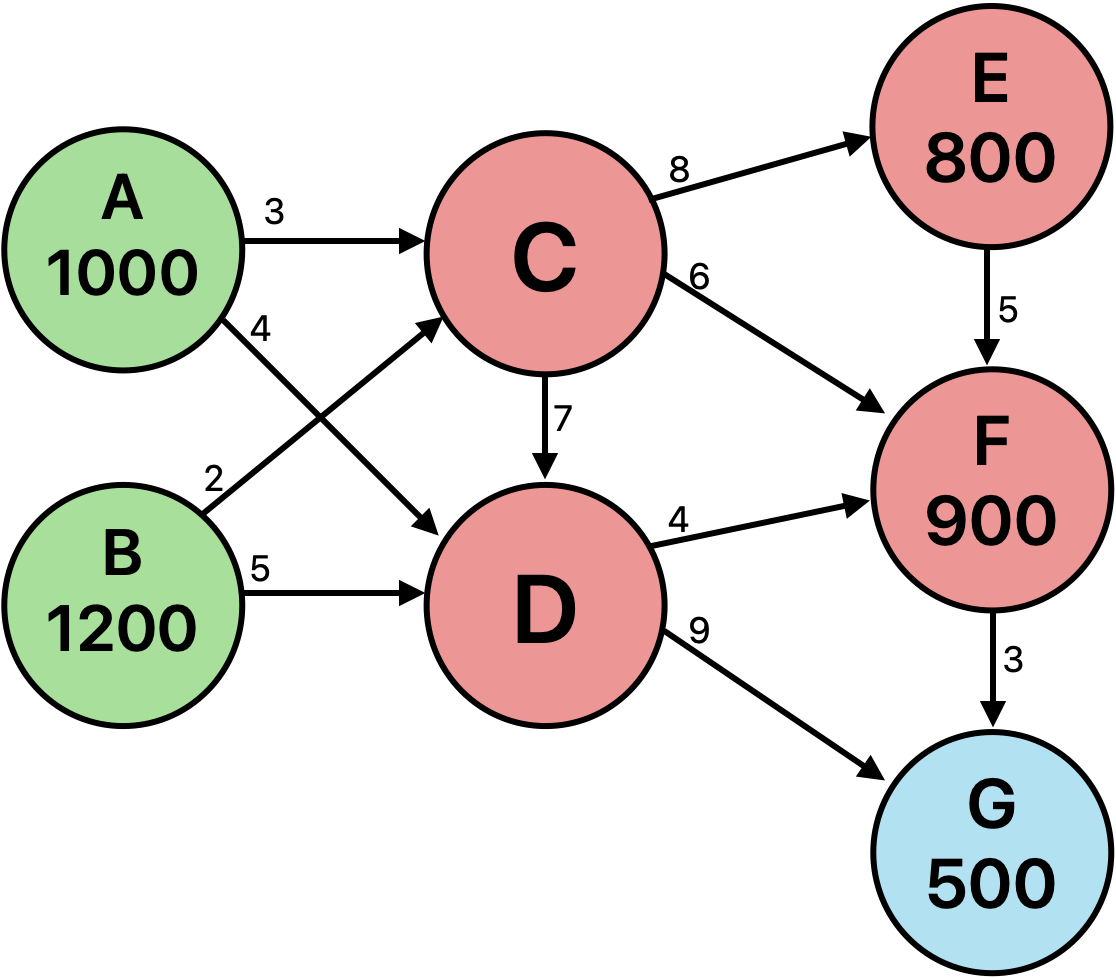
\includegraphics[width=0.8\textwidth]{assets/grafoProb7.png}
\end{figure}

\begin{figure}[H]
\centering
\caption{Tablas para el Problema 7}
\label{fig:tablasolverProb7}
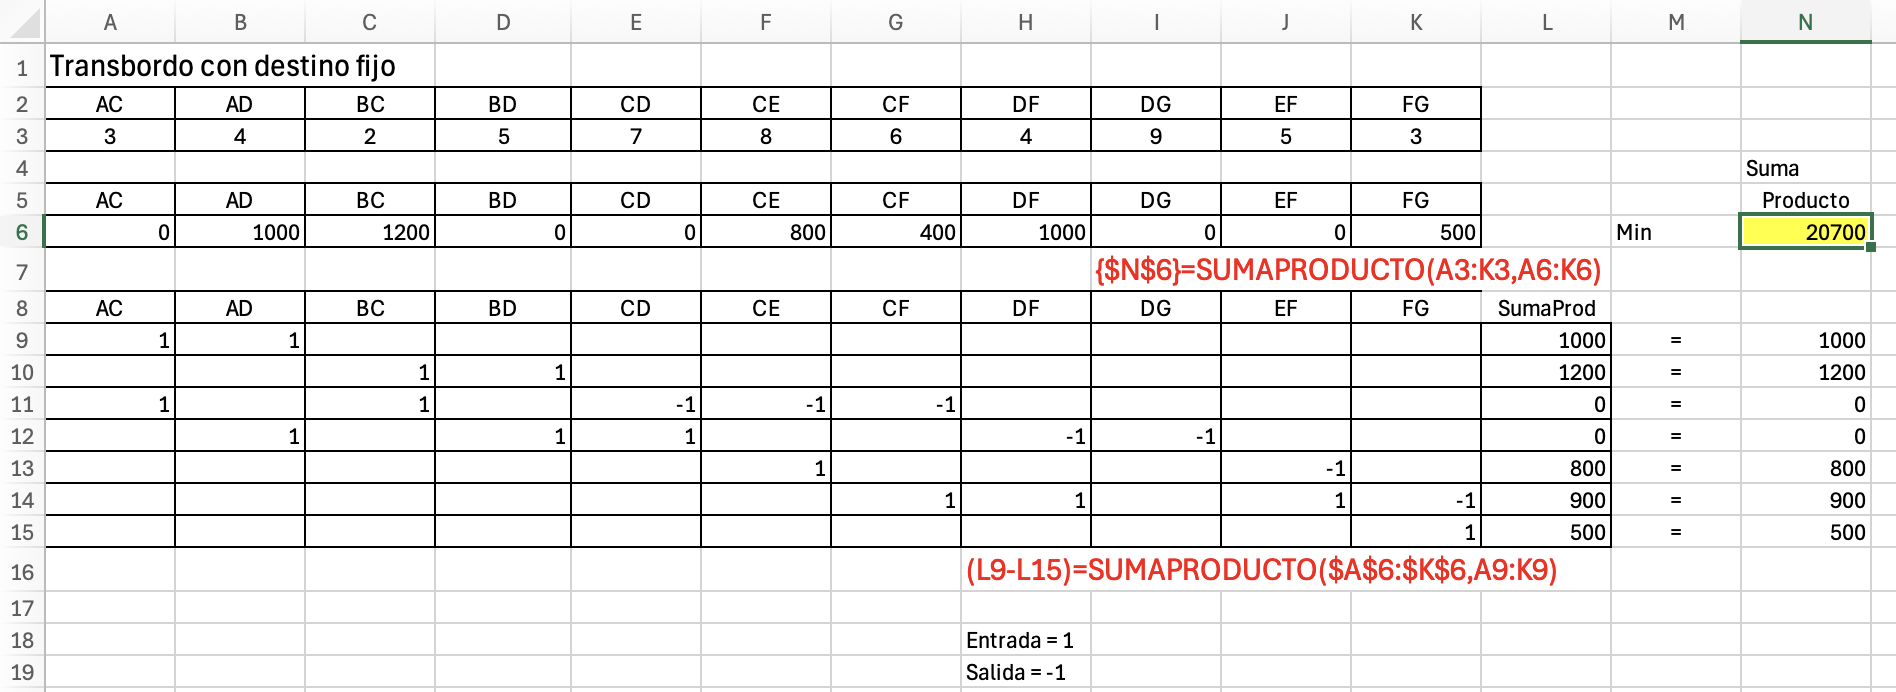
\includegraphics[width=0.8\textwidth]{assets/tablasolverProb7.png}
\end{figure}

Definimos una celda para el resultado, en el que realizamos la SUMPRODUCT de los costos y restricciones y las configuramos en el solver para \underline{minimizar} la función objetivo, como se muestra en la Figura \ref{fig:configSolverProb7}, en la cual obtenemos un costo total de \$20,700.

\begin{figure}[H]
\centering
\caption{Configuración Solver Problema 7}
\label{fig:configSolverProb7}
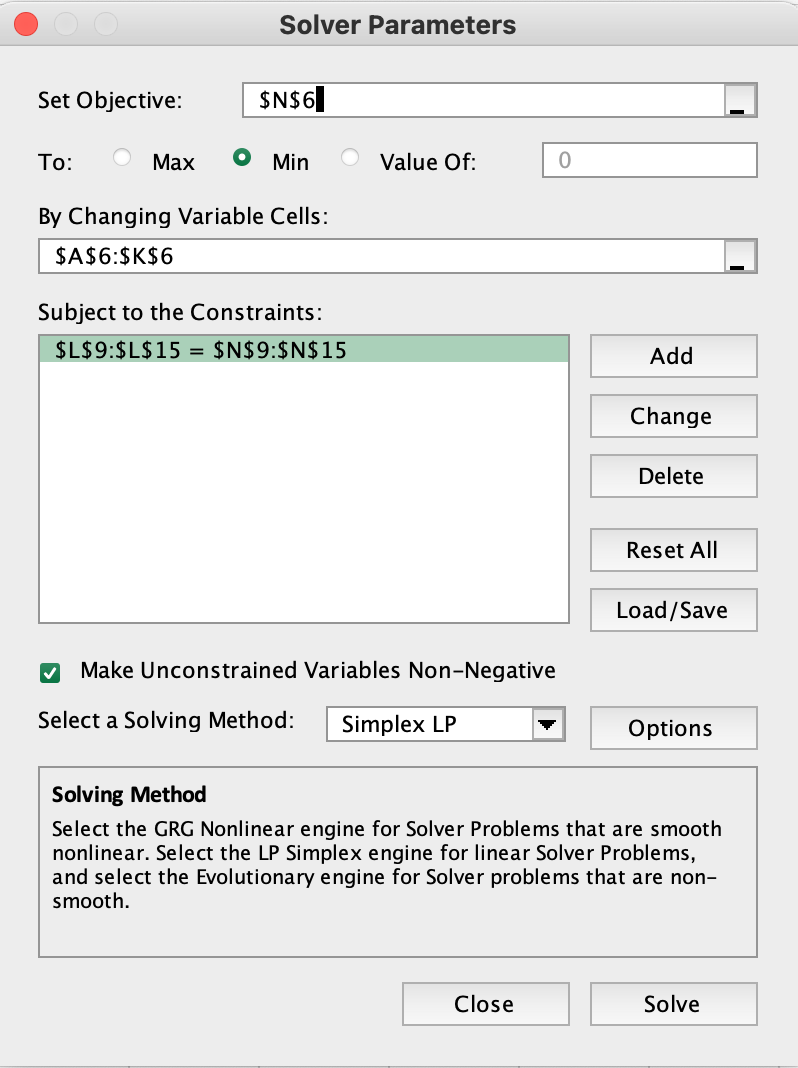
\includegraphics[width=0.6\textwidth]{assets/configSolverProb7.png}
\end{figure}

\section{Asignación}
El problema de asignación es un modelo de programación lineal donde se busca asignar recursos disponibles a tareas de manera que se minimice el costo total, suponiendo que cada recurso se destine a una sola tarea y cada tarea sea ejecutada por un sólo recurso.

Este problema es fundamental en la rama de optimización o investigación operativa en matemáticas y se puede aplicar a la asignación de empleados a tareas, fábricas a productos, vendedores a territorios, postores a contratos, entre otros.

En el contexto de la asignación, el modelado matemático permite formular hipótesis 

Resolvamos el siguiente problema:

Se tienen cuatro actividades y cuatro operarios, los costos se mencionan en la tabla \ref{tab:Prob8}, es decir, el operario 1 hace la actividad con 1 con un costo de 7 (tiempo, precio, etc.).

\begin{table}[H]
\centering
\caption{Problema 8}
\label{tab:Prob8}
\begin{tabular}{ccllcllcllclll}
\multicolumn{14}{c}{Actividad}                                                                                                                                                                                                                                                                                                                                                                                                                                                                                                                                                                                                                                        \\ \cline{2-13}
\multicolumn{1}{c|}{\textbf{Operario}} & \multicolumn{3}{c|}{A1}                                                                                                                        & \multicolumn{3}{c|}{A2}                                                                                                                        & \multicolumn{3}{c|}{A3}                                                                                                                        & \multicolumn{3}{c|}{A4}                                                                                                                        &                          \\ \cline{2-13}
\multicolumn{1}{c|}{Op1}               & \multicolumn{1}{c|}{\cellcolor[HTML]{67FD9A}7} & \multicolumn{1}{l|}{\cellcolor[HTML]{FFCC67}} & \multicolumn{1}{l|}{\cellcolor[HTML]{FCFF2F}} & \multicolumn{1}{c|}{\cellcolor[HTML]{67FD9A}6} & \multicolumn{1}{l|}{\cellcolor[HTML]{FFCC67}} & \multicolumn{1}{l|}{\cellcolor[HTML]{F8FF00}} & \multicolumn{1}{c|}{\cellcolor[HTML]{67FD9A}9} & \multicolumn{1}{l|}{\cellcolor[HTML]{FFCC67}} & \multicolumn{1}{l|}{\cellcolor[HTML]{F8FF00}} & \multicolumn{1}{c|}{\cellcolor[HTML]{67FD9A}2} & \multicolumn{1}{l|}{\cellcolor[HTML]{FFC702}} & \multicolumn{1}{l|}{\cellcolor[HTML]{F8FF00}} & \cellcolor[HTML]{FFCCC9} \\ \cline{2-13}
\multicolumn{1}{c|}{Op2}               & \multicolumn{1}{c|}{\cellcolor[HTML]{67FD9A}7} & \multicolumn{1}{l|}{\cellcolor[HTML]{FFCC67}} & \multicolumn{1}{l|}{\cellcolor[HTML]{FCFF2F}} & \multicolumn{1}{c|}{\cellcolor[HTML]{67FD9A}8} & \multicolumn{1}{l|}{\cellcolor[HTML]{FFCC67}} & \multicolumn{1}{l|}{\cellcolor[HTML]{F8FF00}} & \multicolumn{1}{c|}{\cellcolor[HTML]{67FD9A}5} & \multicolumn{1}{l|}{\cellcolor[HTML]{FFCC67}} & \multicolumn{1}{l|}{\cellcolor[HTML]{F8FF00}} & \multicolumn{1}{c|}{\cellcolor[HTML]{67FD9A}8} & \multicolumn{1}{l|}{\cellcolor[HTML]{FFC702}} & \multicolumn{1}{l|}{\cellcolor[HTML]{F8FF00}} & \cellcolor[HTML]{FFCCC9} \\ \cline{2-13}
\multicolumn{1}{c|}{Op3}               & \multicolumn{1}{c|}{\cellcolor[HTML]{67FD9A}5} & \multicolumn{1}{l|}{\cellcolor[HTML]{FFCC67}} & \multicolumn{1}{l|}{\cellcolor[HTML]{FCFF2F}} & \multicolumn{1}{c|}{\cellcolor[HTML]{67FD9A}4} & \multicolumn{1}{l|}{\cellcolor[HTML]{FFCC67}} & \multicolumn{1}{l|}{\cellcolor[HTML]{F8FF00}} & \multicolumn{1}{c|}{\cellcolor[HTML]{67FD9A}7} & \multicolumn{1}{l|}{\cellcolor[HTML]{FFCC67}} & \multicolumn{1}{l|}{\cellcolor[HTML]{F8FF00}} & \multicolumn{1}{c|}{\cellcolor[HTML]{67FD9A}6} & \multicolumn{1}{l|}{\cellcolor[HTML]{FFC702}} & \multicolumn{1}{l|}{\cellcolor[HTML]{F8FF00}} & \cellcolor[HTML]{FFCCC9} \\ \cline{2-13}
\multicolumn{1}{c|}{Op4}               & \multicolumn{1}{c|}{\cellcolor[HTML]{67FD9A}2} & \multicolumn{1}{l|}{\cellcolor[HTML]{FFCC67}} & \multicolumn{1}{l|}{\cellcolor[HTML]{FCFF2F}} & \multicolumn{1}{c|}{\cellcolor[HTML]{67FD9A}3} & \multicolumn{1}{l|}{\cellcolor[HTML]{FFCC67}} & \multicolumn{1}{l|}{\cellcolor[HTML]{F8FF00}} & \multicolumn{1}{c|}{\cellcolor[HTML]{67FD9A}1} & \multicolumn{1}{l|}{\cellcolor[HTML]{FFCC67}} & \multicolumn{1}{l|}{\cellcolor[HTML]{F8FF00}} & \multicolumn{1}{c|}{\cellcolor[HTML]{67FD9A}8} & \multicolumn{1}{l|}{\cellcolor[HTML]{FFC702}} & \multicolumn{1}{l|}{\cellcolor[HTML]{F8FF00}} & \cellcolor[HTML]{FFCCC9} \\ \cline{2-13}
\multicolumn{1}{l}{}                   & \multicolumn{1}{l}{}                           & \cellcolor[HTML]{FD6864}                      &                                               & \multicolumn{1}{l}{}                           & \cellcolor[HTML]{FD6864}                      &                                               & \multicolumn{1}{l}{}                           & \cellcolor[HTML]{FD6864}                      &                                               & \multicolumn{1}{l}{}                           & \cellcolor[HTML]{FD6864}                      &                                               &                         
\end{tabular}
\end{table}

\textbf{Paso 1.} Para cada fila: Identificamos el número menor de cada fila, y lo indicamos en las celdas exteriores a la derecha junto a cada fila (rosa), como se observa en la Tabla \ref{tab:Paso1Prob8}.

\textbf{Paso 2.} Restarle a cada elemento de la primera subcolumna (verde) de cada fila el número menor de su respectiva fila (rosa) y colocar el resultado en la segunda subcolumna (naranja), como se observa en las Tablas \ref{tab:Paso2.1Prob8} y \ref{tab:Paso2.2Prob8}.

\textbf{Paso 3.} De cada subcolumna central (naranja), selecciona el número menor e indícalo en las celdas exteriores inferiores (rojo), como se observa en la Tabla \ref{tab:Paso3Prob8}.

\textbf{Paso 4.} A cada número de la subcolumna central (naranja), restale el número de su respectiva columna (rojo) y coloca el resultado en las subcolumnas derechas (amarillo), como se observa en las Tablas \ref{tab:Paso4.1Prob8} y \ref{tab:Paso4.2Prob8}.

\textbf{Paso 5.} Nos interesan los ceros en las subcolumnas derechas (amarillo), pues son costos mínimos. Será en estos donde podremos asignar tareas a operarios. Asignamos entonces las tareas con los siguientes criterios:

\textbf{Paso 5.1.} Comenzamos asignando aquellas tareas que sólo puede hacer un operario, es decir, aquellas filas que sólo tengan un 0 en la subcolumna derecha, como es el caso de la tarea 3 al operario 2, lo que bloquea al operario (fila) y la tarea (columna) de ser elegidos; como se observa en la Tabla \ref{tab:Paso5.1.1Prob8}. 
Posteriormente, sólo queda disponible la terea 4 para el operario 1, lo que también los bloquea; como se observa en la Tabla \ref{tab:Paso5.1.2Prob8}.
Posteriormente, sólo queda disponible la tarea 1 para el operario 4, lo que también lo bloquea, como se observa en la Tabla \ref{tab:Paso5.1.3Prob8}.
Finalmente, sólo queda desiponible la tarea 2 para el operario 3, por lo que se la asignamos; como se observa en la Tabla \ref{tab:Paso5.1.4Prob8} y terminamos con el procedimiento.

\textbf{Paso 5.2.} En caso de que se llegara a dar un empate, cuando no existe forma de asignar por bloqueo y eliminación, asignar la tarea al operario con el costo mínimo (verde)\footnote{Aunque en este caso no fue necesario.}.


\begin{table}[H]
\centering
\caption{Paso 1 Problema 8}
\label{tab:Paso1Prob8}
\begin{tabular}{ccllcllcllcllc}
\multicolumn{14}{c}{Actividad}                                                                                                                                                                                                                                                                                                                                                                                                                                                                                                                                                                                                                                         \\ \cline{2-13}
\multicolumn{1}{c|}{\textbf{Operario}} & \multicolumn{3}{c|}{A1}                                                                                                                        & \multicolumn{3}{c|}{A2}                                                                                                                        & \multicolumn{3}{c|}{A3}                                                                                                                        & \multicolumn{3}{c|}{A4}                                                                                                                        & \multicolumn{1}{l}{}      \\ \cline{2-13}
\multicolumn{1}{c|}{Op1}               & \multicolumn{1}{c|}{\cellcolor[HTML]{67FD9A}7} & \multicolumn{1}{l|}{\cellcolor[HTML]{FFCC67}} & \multicolumn{1}{l|}{\cellcolor[HTML]{FCFF2F}} & \multicolumn{1}{c|}{\cellcolor[HTML]{67FD9A}6} & \multicolumn{1}{l|}{\cellcolor[HTML]{FFCC67}} & \multicolumn{1}{l|}{\cellcolor[HTML]{F8FF00}} & \multicolumn{1}{c|}{\cellcolor[HTML]{67FD9A}9} & \multicolumn{1}{l|}{\cellcolor[HTML]{FFCC67}} & \multicolumn{1}{l|}{\cellcolor[HTML]{F8FF00}} & \multicolumn{1}{c|}{\cellcolor[HTML]{67FD9A}2} & \multicolumn{1}{l|}{\cellcolor[HTML]{FFC702}} & \multicolumn{1}{l|}{\cellcolor[HTML]{F8FF00}} & \cellcolor[HTML]{FFCCC9}2 \\ \cline{2-13}
\multicolumn{1}{c|}{Op2}               & \multicolumn{1}{c|}{\cellcolor[HTML]{67FD9A}7} & \multicolumn{1}{l|}{\cellcolor[HTML]{FFCC67}} & \multicolumn{1}{l|}{\cellcolor[HTML]{FCFF2F}} & \multicolumn{1}{c|}{\cellcolor[HTML]{67FD9A}8} & \multicolumn{1}{l|}{\cellcolor[HTML]{FFCC67}} & \multicolumn{1}{l|}{\cellcolor[HTML]{F8FF00}} & \multicolumn{1}{c|}{\cellcolor[HTML]{67FD9A}5} & \multicolumn{1}{l|}{\cellcolor[HTML]{FFCC67}} & \multicolumn{1}{l|}{\cellcolor[HTML]{F8FF00}} & \multicolumn{1}{c|}{\cellcolor[HTML]{67FD9A}8} & \multicolumn{1}{l|}{\cellcolor[HTML]{FFC702}} & \multicolumn{1}{l|}{\cellcolor[HTML]{F8FF00}} & \cellcolor[HTML]{FFCCC9}5 \\ \cline{2-13}
\multicolumn{1}{c|}{Op3}               & \multicolumn{1}{c|}{\cellcolor[HTML]{67FD9A}5} & \multicolumn{1}{l|}{\cellcolor[HTML]{FFCC67}} & \multicolumn{1}{l|}{\cellcolor[HTML]{FCFF2F}} & \multicolumn{1}{c|}{\cellcolor[HTML]{67FD9A}4} & \multicolumn{1}{l|}{\cellcolor[HTML]{FFCC67}} & \multicolumn{1}{l|}{\cellcolor[HTML]{F8FF00}} & \multicolumn{1}{c|}{\cellcolor[HTML]{67FD9A}7} & \multicolumn{1}{l|}{\cellcolor[HTML]{FFCC67}} & \multicolumn{1}{l|}{\cellcolor[HTML]{F8FF00}} & \multicolumn{1}{c|}{\cellcolor[HTML]{67FD9A}6} & \multicolumn{1}{l|}{\cellcolor[HTML]{FFC702}} & \multicolumn{1}{l|}{\cellcolor[HTML]{F8FF00}} & \cellcolor[HTML]{FFCCC9}4 \\ \cline{2-13}
\multicolumn{1}{c|}{Op4}               & \multicolumn{1}{c|}{\cellcolor[HTML]{67FD9A}2} & \multicolumn{1}{l|}{\cellcolor[HTML]{FFCC67}} & \multicolumn{1}{l|}{\cellcolor[HTML]{FCFF2F}} & \multicolumn{1}{c|}{\cellcolor[HTML]{67FD9A}3} & \multicolumn{1}{l|}{\cellcolor[HTML]{FFCC67}} & \multicolumn{1}{l|}{\cellcolor[HTML]{F8FF00}} & \multicolumn{1}{c|}{\cellcolor[HTML]{67FD9A}1} & \multicolumn{1}{l|}{\cellcolor[HTML]{FFCC67}} & \multicolumn{1}{l|}{\cellcolor[HTML]{F8FF00}} & \multicolumn{1}{c|}{\cellcolor[HTML]{67FD9A}8} & \multicolumn{1}{l|}{\cellcolor[HTML]{FFC702}} & \multicolumn{1}{l|}{\cellcolor[HTML]{F8FF00}} & \cellcolor[HTML]{FFCCC9}1 \\ \cline{2-13}
\multicolumn{1}{l}{}                   & \multicolumn{1}{l}{}                           & \cellcolor[HTML]{FD6864}                      &                                               & \multicolumn{1}{l}{}                           & \cellcolor[HTML]{FD6864}                      &                                               & \multicolumn{1}{l}{}                           & \cellcolor[HTML]{FD6864}                      &                                               & \multicolumn{1}{l}{}                           & \cellcolor[HTML]{FD6864}                      &                                               & \multicolumn{1}{l}{}     
\end{tabular}
\end{table}

\begin{table}[H]
\centering
\caption{Paso 2.1 Problema 8}
\label{tab:Paso2.1Prob8}
\begin{tabular}{ccclcclcclcclc}
\multicolumn{14}{c}{Actividad}                                                                                                                                                                                                                                                                                                                                                                                                                                                                                                                                                                                                                                                     \\ \cline{2-13}
\multicolumn{1}{c|}{\textbf{Operario}} & \multicolumn{3}{c|}{A1}                                                                                                                           & \multicolumn{3}{c|}{A2}                                                                                                                           & \multicolumn{3}{c|}{A3}                                                                                                                           & \multicolumn{3}{c|}{A4}                                                                                                                           & \multicolumn{1}{l}{}      \\ \cline{2-13}
\multicolumn{1}{c|}{Op1}               & \multicolumn{1}{c|}{\cellcolor[HTML]{67FD9A}7} & \multicolumn{1}{c|}{\cellcolor[HTML]{FFCC67}7-2} & \multicolumn{1}{l|}{\cellcolor[HTML]{FCFF2F}} & \multicolumn{1}{c|}{\cellcolor[HTML]{67FD9A}6} & \multicolumn{1}{c|}{\cellcolor[HTML]{FFCC67}6-2} & \multicolumn{1}{l|}{\cellcolor[HTML]{F8FF00}} & \multicolumn{1}{c|}{\cellcolor[HTML]{67FD9A}9} & \multicolumn{1}{c|}{\cellcolor[HTML]{FFCC67}9-2} & \multicolumn{1}{l|}{\cellcolor[HTML]{F8FF00}} & \multicolumn{1}{c|}{\cellcolor[HTML]{67FD9A}2} & \multicolumn{1}{c|}{\cellcolor[HTML]{FFC702}2-2} & \multicolumn{1}{l|}{\cellcolor[HTML]{F8FF00}} & \cellcolor[HTML]{FFCCC9}2 \\ \cline{2-13}
\multicolumn{1}{c|}{Op2}               & \multicolumn{1}{c|}{\cellcolor[HTML]{67FD9A}7} & \multicolumn{1}{c|}{\cellcolor[HTML]{FFCC67}7-5} & \multicolumn{1}{l|}{\cellcolor[HTML]{FCFF2F}} & \multicolumn{1}{c|}{\cellcolor[HTML]{67FD9A}8} & \multicolumn{1}{c|}{\cellcolor[HTML]{FFCC67}8-5} & \multicolumn{1}{l|}{\cellcolor[HTML]{F8FF00}} & \multicolumn{1}{c|}{\cellcolor[HTML]{67FD9A}5} & \multicolumn{1}{c|}{\cellcolor[HTML]{FFCC67}5-5} & \multicolumn{1}{l|}{\cellcolor[HTML]{F8FF00}} & \multicolumn{1}{c|}{\cellcolor[HTML]{67FD9A}8} & \multicolumn{1}{c|}{\cellcolor[HTML]{FFC702}8-5} & \multicolumn{1}{l|}{\cellcolor[HTML]{F8FF00}} & \cellcolor[HTML]{FFCCC9}5 \\ \cline{2-13}
\multicolumn{1}{c|}{Op3}               & \multicolumn{1}{c|}{\cellcolor[HTML]{67FD9A}5} & \multicolumn{1}{c|}{\cellcolor[HTML]{FFCC67}5-4} & \multicolumn{1}{l|}{\cellcolor[HTML]{FCFF2F}} & \multicolumn{1}{c|}{\cellcolor[HTML]{67FD9A}4} & \multicolumn{1}{c|}{\cellcolor[HTML]{FFCC67}4-4} & \multicolumn{1}{l|}{\cellcolor[HTML]{F8FF00}} & \multicolumn{1}{c|}{\cellcolor[HTML]{67FD9A}7} & \multicolumn{1}{c|}{\cellcolor[HTML]{FFCC67}7-4} & \multicolumn{1}{l|}{\cellcolor[HTML]{F8FF00}} & \multicolumn{1}{c|}{\cellcolor[HTML]{67FD9A}6} & \multicolumn{1}{c|}{\cellcolor[HTML]{FFC702}6-4} & \multicolumn{1}{l|}{\cellcolor[HTML]{F8FF00}} & \cellcolor[HTML]{FFCCC9}4 \\ \cline{2-13}
\multicolumn{1}{c|}{Op4}               & \multicolumn{1}{c|}{\cellcolor[HTML]{67FD9A}2} & \multicolumn{1}{c|}{\cellcolor[HTML]{FFCC67}2-1} & \multicolumn{1}{l|}{\cellcolor[HTML]{FCFF2F}} & \multicolumn{1}{c|}{\cellcolor[HTML]{67FD9A}3} & \multicolumn{1}{c|}{\cellcolor[HTML]{FFCC67}3-1} & \multicolumn{1}{l|}{\cellcolor[HTML]{F8FF00}} & \multicolumn{1}{c|}{\cellcolor[HTML]{67FD9A}1} & \multicolumn{1}{c|}{\cellcolor[HTML]{FFCC67}1-1} & \multicolumn{1}{l|}{\cellcolor[HTML]{F8FF00}} & \multicolumn{1}{c|}{\cellcolor[HTML]{67FD9A}8} & \multicolumn{1}{c|}{\cellcolor[HTML]{FFC702}8-1} & \multicolumn{1}{l|}{\cellcolor[HTML]{F8FF00}} & \cellcolor[HTML]{FFCCC9}1 \\ \cline{2-13}
\multicolumn{1}{l}{}                   & \multicolumn{1}{l}{}                           & \multicolumn{1}{l}{\cellcolor[HTML]{FD6864}}     &                                               & \multicolumn{1}{l}{}                           & \multicolumn{1}{l}{\cellcolor[HTML]{FD6864}}     &                                               & \multicolumn{1}{l}{}                           & \multicolumn{1}{l}{\cellcolor[HTML]{FD6864}}     &                                               & \multicolumn{1}{l}{}                           & \multicolumn{1}{l}{\cellcolor[HTML]{FD6864}}     &                                               & \multicolumn{1}{l}{}     
\end{tabular}
\end{table}

\begin{table}[H]
\centering
\caption{Paso 2.2 Problema 8}
\label{tab:Paso2.2Prob8}
\begin{tabular}{ccclcclcclcclc}
\multicolumn{14}{c}{Actividad}                                                                                                                                                                                                                                                                                                                                                                                                                                                                                                                                                                                                                                             \\ \cline{2-13}
\multicolumn{1}{c|}{\textbf{Operario}} & \multicolumn{3}{c|}{A1}                                                                                                                         & \multicolumn{3}{c|}{A2}                                                                                                                         & \multicolumn{3}{c|}{A3}                                                                                                                         & \multicolumn{3}{c|}{A4}                                                                                                                         & \multicolumn{1}{l}{}      \\ \cline{2-13}
\multicolumn{1}{c|}{Op1}               & \multicolumn{1}{c|}{\cellcolor[HTML]{67FD9A}7} & \multicolumn{1}{c|}{\cellcolor[HTML]{FFCC67}5} & \multicolumn{1}{l|}{\cellcolor[HTML]{FCFF2F}} & \multicolumn{1}{c|}{\cellcolor[HTML]{67FD9A}6} & \multicolumn{1}{c|}{\cellcolor[HTML]{FFCC67}4} & \multicolumn{1}{l|}{\cellcolor[HTML]{F8FF00}} & \multicolumn{1}{c|}{\cellcolor[HTML]{67FD9A}9} & \multicolumn{1}{c|}{\cellcolor[HTML]{FFCC67}7} & \multicolumn{1}{l|}{\cellcolor[HTML]{F8FF00}} & \multicolumn{1}{c|}{\cellcolor[HTML]{67FD9A}2} & \multicolumn{1}{c|}{\cellcolor[HTML]{FFC702}0} & \multicolumn{1}{l|}{\cellcolor[HTML]{F8FF00}} & \cellcolor[HTML]{FFCCC9}2 \\ \cline{2-13}
\multicolumn{1}{c|}{Op2}               & \multicolumn{1}{c|}{\cellcolor[HTML]{67FD9A}7} & \multicolumn{1}{c|}{\cellcolor[HTML]{FFCC67}2} & \multicolumn{1}{l|}{\cellcolor[HTML]{FCFF2F}} & \multicolumn{1}{c|}{\cellcolor[HTML]{67FD9A}8} & \multicolumn{1}{c|}{\cellcolor[HTML]{FFCC67}3} & \multicolumn{1}{l|}{\cellcolor[HTML]{F8FF00}} & \multicolumn{1}{c|}{\cellcolor[HTML]{67FD9A}5} & \multicolumn{1}{c|}{\cellcolor[HTML]{FFCC67}0} & \multicolumn{1}{l|}{\cellcolor[HTML]{F8FF00}} & \multicolumn{1}{c|}{\cellcolor[HTML]{67FD9A}8} & \multicolumn{1}{c|}{\cellcolor[HTML]{FFC702}3} & \multicolumn{1}{l|}{\cellcolor[HTML]{F8FF00}} & \cellcolor[HTML]{FFCCC9}5 \\ \cline{2-13}
\multicolumn{1}{c|}{Op3}               & \multicolumn{1}{c|}{\cellcolor[HTML]{67FD9A}5} & \multicolumn{1}{c|}{\cellcolor[HTML]{FFCC67}1} & \multicolumn{1}{l|}{\cellcolor[HTML]{FCFF2F}} & \multicolumn{1}{c|}{\cellcolor[HTML]{67FD9A}4} & \multicolumn{1}{c|}{\cellcolor[HTML]{FFCC67}0} & \multicolumn{1}{l|}{\cellcolor[HTML]{F8FF00}} & \multicolumn{1}{c|}{\cellcolor[HTML]{67FD9A}7} & \multicolumn{1}{c|}{\cellcolor[HTML]{FFCC67}3} & \multicolumn{1}{l|}{\cellcolor[HTML]{F8FF00}} & \multicolumn{1}{c|}{\cellcolor[HTML]{67FD9A}6} & \multicolumn{1}{c|}{\cellcolor[HTML]{FFC702}2} & \multicolumn{1}{l|}{\cellcolor[HTML]{F8FF00}} & \cellcolor[HTML]{FFCCC9}4 \\ \cline{2-13}
\multicolumn{1}{c|}{Op4}               & \multicolumn{1}{c|}{\cellcolor[HTML]{67FD9A}2} & \multicolumn{1}{c|}{\cellcolor[HTML]{FFCC67}1} & \multicolumn{1}{l|}{\cellcolor[HTML]{FCFF2F}} & \multicolumn{1}{c|}{\cellcolor[HTML]{67FD9A}3} & \multicolumn{1}{c|}{\cellcolor[HTML]{FFCC67}2} & \multicolumn{1}{l|}{\cellcolor[HTML]{F8FF00}} & \multicolumn{1}{c|}{\cellcolor[HTML]{67FD9A}1} & \multicolumn{1}{c|}{\cellcolor[HTML]{FFCC67}0} & \multicolumn{1}{l|}{\cellcolor[HTML]{F8FF00}} & \multicolumn{1}{c|}{\cellcolor[HTML]{67FD9A}8} & \multicolumn{1}{c|}{\cellcolor[HTML]{FFC702}7} & \multicolumn{1}{l|}{\cellcolor[HTML]{F8FF00}} & \cellcolor[HTML]{FFCCC9}1 \\ \cline{2-13}
\multicolumn{1}{l}{}                   & \multicolumn{1}{l}{}                           & \multicolumn{1}{l}{\cellcolor[HTML]{FD6864}}   &                                               & \multicolumn{1}{l}{}                           & \multicolumn{1}{l}{\cellcolor[HTML]{FD6864}}   &                                               & \multicolumn{1}{l}{}                           & \multicolumn{1}{l}{\cellcolor[HTML]{FD6864}}   &                                               & \multicolumn{1}{l}{}                           & \multicolumn{1}{l}{\cellcolor[HTML]{FD6864}}   &                                               & \multicolumn{1}{l}{}     
\end{tabular}
\end{table}

\begin{table}[H]
\centering
\caption{Paso 3 Problema 8}
\label{tab:Paso3Prob8}
\begin{tabular}{ccclcclcclcclc}
\multicolumn{14}{c}{Actividad}                                                                                                                                                                                                                                                                                                                                                                                                                                                                                                                                                                                                                                             \\ \cline{2-13}
\multicolumn{1}{c|}{\textbf{Operario}} & \multicolumn{3}{c|}{A1}                                                                                                                         & \multicolumn{3}{c|}{A2}                                                                                                                         & \multicolumn{3}{c|}{A3}                                                                                                                         & \multicolumn{3}{c|}{A4}                                                                                                                         & \multicolumn{1}{l}{}      \\ \cline{2-13}
\multicolumn{1}{c|}{Op1}               & \multicolumn{1}{c|}{\cellcolor[HTML]{67FD9A}7} & \multicolumn{1}{c|}{\cellcolor[HTML]{FFCC67}5} & \multicolumn{1}{l|}{\cellcolor[HTML]{FCFF2F}} & \multicolumn{1}{c|}{\cellcolor[HTML]{67FD9A}6} & \multicolumn{1}{c|}{\cellcolor[HTML]{FFCC67}4} & \multicolumn{1}{l|}{\cellcolor[HTML]{F8FF00}} & \multicolumn{1}{c|}{\cellcolor[HTML]{67FD9A}9} & \multicolumn{1}{c|}{\cellcolor[HTML]{FFCC67}7} & \multicolumn{1}{l|}{\cellcolor[HTML]{F8FF00}} & \multicolumn{1}{c|}{\cellcolor[HTML]{67FD9A}2} & \multicolumn{1}{c|}{\cellcolor[HTML]{FFC702}0} & \multicolumn{1}{l|}{\cellcolor[HTML]{F8FF00}} & \cellcolor[HTML]{FFCCC9}2 \\ \cline{2-13}
\multicolumn{1}{c|}{Op2}               & \multicolumn{1}{c|}{\cellcolor[HTML]{67FD9A}7} & \multicolumn{1}{c|}{\cellcolor[HTML]{FFCC67}2} & \multicolumn{1}{l|}{\cellcolor[HTML]{FCFF2F}} & \multicolumn{1}{c|}{\cellcolor[HTML]{67FD9A}8} & \multicolumn{1}{c|}{\cellcolor[HTML]{FFCC67}3} & \multicolumn{1}{l|}{\cellcolor[HTML]{F8FF00}} & \multicolumn{1}{c|}{\cellcolor[HTML]{67FD9A}5} & \multicolumn{1}{c|}{\cellcolor[HTML]{FFCC67}0} & \multicolumn{1}{l|}{\cellcolor[HTML]{F8FF00}} & \multicolumn{1}{c|}{\cellcolor[HTML]{67FD9A}8} & \multicolumn{1}{c|}{\cellcolor[HTML]{FFC702}3} & \multicolumn{1}{l|}{\cellcolor[HTML]{F8FF00}} & \cellcolor[HTML]{FFCCC9}5 \\ \cline{2-13}
\multicolumn{1}{c|}{Op3}               & \multicolumn{1}{c|}{\cellcolor[HTML]{67FD9A}5} & \multicolumn{1}{c|}{\cellcolor[HTML]{FFCC67}1} & \multicolumn{1}{l|}{\cellcolor[HTML]{FCFF2F}} & \multicolumn{1}{c|}{\cellcolor[HTML]{67FD9A}4} & \multicolumn{1}{c|}{\cellcolor[HTML]{FFCC67}0} & \multicolumn{1}{l|}{\cellcolor[HTML]{F8FF00}} & \multicolumn{1}{c|}{\cellcolor[HTML]{67FD9A}7} & \multicolumn{1}{c|}{\cellcolor[HTML]{FFCC67}3} & \multicolumn{1}{l|}{\cellcolor[HTML]{F8FF00}} & \multicolumn{1}{c|}{\cellcolor[HTML]{67FD9A}6} & \multicolumn{1}{c|}{\cellcolor[HTML]{FFC702}2} & \multicolumn{1}{l|}{\cellcolor[HTML]{F8FF00}} & \cellcolor[HTML]{FFCCC9}4 \\ \cline{2-13}
\multicolumn{1}{c|}{Op4}               & \multicolumn{1}{c|}{\cellcolor[HTML]{67FD9A}2} & \multicolumn{1}{c|}{\cellcolor[HTML]{FFCC67}1} & \multicolumn{1}{l|}{\cellcolor[HTML]{FCFF2F}} & \multicolumn{1}{c|}{\cellcolor[HTML]{67FD9A}3} & \multicolumn{1}{c|}{\cellcolor[HTML]{FFCC67}2} & \multicolumn{1}{l|}{\cellcolor[HTML]{F8FF00}} & \multicolumn{1}{c|}{\cellcolor[HTML]{67FD9A}1} & \multicolumn{1}{c|}{\cellcolor[HTML]{FFCC67}0} & \multicolumn{1}{l|}{\cellcolor[HTML]{F8FF00}} & \multicolumn{1}{c|}{\cellcolor[HTML]{67FD9A}8} & \multicolumn{1}{c|}{\cellcolor[HTML]{FFC702}7} & \multicolumn{1}{l|}{\cellcolor[HTML]{F8FF00}} & \cellcolor[HTML]{FFCCC9}1 \\ \cline{2-13}
\multicolumn{1}{l}{}                   &                                                & \cellcolor[HTML]{FD6864}1                      & \multicolumn{1}{c}{}                          &                                                & \cellcolor[HTML]{FD6864}0                      & \multicolumn{1}{c}{}                          &                                                & \cellcolor[HTML]{FD6864}0                      & \multicolumn{1}{c}{}                          &                                                & \cellcolor[HTML]{FD6864}0                      &                                               & \multicolumn{1}{l}{}     
\end{tabular}
\end{table}

\begin{table}[H]
\centering
\caption{Paso 4.1 Problema 8}
\label{tab:Paso4.1Prob8}
\begin{tabular}{ccclcclcclcclc}
\multicolumn{14}{c}{Actividad}                                                                                                                                                                                                                                                                                                                                                                                                                                                                                                                                                                                                                                                         \\ \cline{2-13}
\multicolumn{1}{c|}{\textbf{Operario}} & \multicolumn{3}{c|}{A1}                                                                                                                            & \multicolumn{3}{c|}{A2}                                                                                                                            & \multicolumn{3}{c|}{A3}                                                                                                                            & \multicolumn{3}{c|}{A4}                                                                                                                            & \multicolumn{1}{l}{}      \\ \cline{2-13}
\multicolumn{1}{c|}{Op1}               & \multicolumn{1}{c|}{\cellcolor[HTML]{67FD9A}7} & \multicolumn{1}{c|}{\cellcolor[HTML]{FFCC67}5} & \multicolumn{1}{l|}{\cellcolor[HTML]{FCFF2F}5-1} & \multicolumn{1}{c|}{\cellcolor[HTML]{67FD9A}6} & \multicolumn{1}{c|}{\cellcolor[HTML]{FFCC67}4} & \multicolumn{1}{l|}{\cellcolor[HTML]{F8FF00}4-0} & \multicolumn{1}{c|}{\cellcolor[HTML]{67FD9A}9} & \multicolumn{1}{c|}{\cellcolor[HTML]{FFCC67}7} & \multicolumn{1}{l|}{\cellcolor[HTML]{F8FF00}7-0} & \multicolumn{1}{c|}{\cellcolor[HTML]{67FD9A}2} & \multicolumn{1}{c|}{\cellcolor[HTML]{FFC702}0} & \multicolumn{1}{l|}{\cellcolor[HTML]{F8FF00}0-0} & \cellcolor[HTML]{FFCCC9}2 \\ \cline{2-13}
\multicolumn{1}{c|}{Op2}               & \multicolumn{1}{c|}{\cellcolor[HTML]{67FD9A}7} & \multicolumn{1}{c|}{\cellcolor[HTML]{FFCC67}2} & \multicolumn{1}{l|}{\cellcolor[HTML]{FCFF2F}2-1} & \multicolumn{1}{c|}{\cellcolor[HTML]{67FD9A}8} & \multicolumn{1}{c|}{\cellcolor[HTML]{FFCC67}3} & \multicolumn{1}{l|}{\cellcolor[HTML]{F8FF00}3-0} & \multicolumn{1}{c|}{\cellcolor[HTML]{67FD9A}5} & \multicolumn{1}{c|}{\cellcolor[HTML]{FFCC67}0} & \multicolumn{1}{l|}{\cellcolor[HTML]{F8FF00}0-0} & \multicolumn{1}{c|}{\cellcolor[HTML]{67FD9A}8} & \multicolumn{1}{c|}{\cellcolor[HTML]{FFC702}3} & \multicolumn{1}{l|}{\cellcolor[HTML]{F8FF00}3-0} & \cellcolor[HTML]{FFCCC9}5 \\ \cline{2-13}
\multicolumn{1}{c|}{Op3}               & \multicolumn{1}{c|}{\cellcolor[HTML]{67FD9A}5} & \multicolumn{1}{c|}{\cellcolor[HTML]{FFCC67}1} & \multicolumn{1}{l|}{\cellcolor[HTML]{FCFF2F}1-1} & \multicolumn{1}{c|}{\cellcolor[HTML]{67FD9A}4} & \multicolumn{1}{c|}{\cellcolor[HTML]{FFCC67}0} & \multicolumn{1}{l|}{\cellcolor[HTML]{F8FF00}0-0} & \multicolumn{1}{c|}{\cellcolor[HTML]{67FD9A}7} & \multicolumn{1}{c|}{\cellcolor[HTML]{FFCC67}3} & \multicolumn{1}{l|}{\cellcolor[HTML]{F8FF00}3-0} & \multicolumn{1}{c|}{\cellcolor[HTML]{67FD9A}6} & \multicolumn{1}{c|}{\cellcolor[HTML]{FFC702}2} & \multicolumn{1}{l|}{\cellcolor[HTML]{F8FF00}2-0} & \cellcolor[HTML]{FFCCC9}4 \\ \cline{2-13}
\multicolumn{1}{c|}{Op4}               & \multicolumn{1}{c|}{\cellcolor[HTML]{67FD9A}2} & \multicolumn{1}{c|}{\cellcolor[HTML]{FFCC67}1} & \multicolumn{1}{l|}{\cellcolor[HTML]{FCFF2F}1-1} & \multicolumn{1}{c|}{\cellcolor[HTML]{67FD9A}3} & \multicolumn{1}{c|}{\cellcolor[HTML]{FFCC67}2} & \multicolumn{1}{l|}{\cellcolor[HTML]{F8FF00}2-0} & \multicolumn{1}{c|}{\cellcolor[HTML]{67FD9A}1} & \multicolumn{1}{c|}{\cellcolor[HTML]{FFCC67}0} & \multicolumn{1}{l|}{\cellcolor[HTML]{F8FF00}0-0} & \multicolumn{1}{c|}{\cellcolor[HTML]{67FD9A}8} & \multicolumn{1}{c|}{\cellcolor[HTML]{FFC702}7} & \multicolumn{1}{l|}{\cellcolor[HTML]{F8FF00}7-0} & \cellcolor[HTML]{FFCCC9}1 \\ \cline{2-13}
\multicolumn{1}{l}{}                   &                                                & \cellcolor[HTML]{FD6864}1                      & \multicolumn{1}{c}{}                             &                                                & \cellcolor[HTML]{FD6864}0                      & \multicolumn{1}{c}{}                             &                                                & \cellcolor[HTML]{FD6864}0                      & \multicolumn{1}{c}{}                             &                                                & \cellcolor[HTML]{FD6864}0                      &                                                  & \multicolumn{1}{l}{}     
\end{tabular}
\end{table}

\begin{table}[H]
\centering
\caption{Paso 4.2 Problema 8}
\label{tab:Paso4.2Prob8}
\begin{tabular}{cccccccccccccc}
\multicolumn{14}{c}{Actividad}                                                                                                                                                                                                                                                                                                                                                                                                                                                                                                                                                                                                                                                 \\ \cline{2-13}
\multicolumn{1}{c|}{\textbf{Operario}} & \multicolumn{3}{c|}{A1}                                                                                                                          & \multicolumn{3}{c|}{A2}                                                                                                                          & \multicolumn{3}{c|}{A3}                                                                                                                          & \multicolumn{3}{c|}{A4}                                                                                                                          & \multicolumn{1}{l}{}      \\ \cline{2-13}
\multicolumn{1}{c|}{Op1}               & \multicolumn{1}{c|}{\cellcolor[HTML]{67FD9A}7} & \multicolumn{1}{c|}{\cellcolor[HTML]{FFCC67}5} & \multicolumn{1}{c|}{\cellcolor[HTML]{FCFF2F}4} & \multicolumn{1}{c|}{\cellcolor[HTML]{67FD9A}6} & \multicolumn{1}{c|}{\cellcolor[HTML]{FFCC67}4} & \multicolumn{1}{c|}{\cellcolor[HTML]{F8FF00}4} & \multicolumn{1}{c|}{\cellcolor[HTML]{67FD9A}9} & \multicolumn{1}{c|}{\cellcolor[HTML]{FFCC67}7} & \multicolumn{1}{c|}{\cellcolor[HTML]{F8FF00}7} & \multicolumn{1}{c|}{\cellcolor[HTML]{67FD9A}2} & \multicolumn{1}{c|}{\cellcolor[HTML]{FFC702}0} & \multicolumn{1}{c|}{\cellcolor[HTML]{F8FF00}0} & \cellcolor[HTML]{FFCCC9}2 \\ \cline{2-13}
\multicolumn{1}{c|}{Op2}               & \multicolumn{1}{c|}{\cellcolor[HTML]{67FD9A}7} & \multicolumn{1}{c|}{\cellcolor[HTML]{FFCC67}2} & \multicolumn{1}{c|}{\cellcolor[HTML]{FCFF2F}1} & \multicolumn{1}{c|}{\cellcolor[HTML]{67FD9A}8} & \multicolumn{1}{c|}{\cellcolor[HTML]{FFCC67}3} & \multicolumn{1}{c|}{\cellcolor[HTML]{F8FF00}3} & \multicolumn{1}{c|}{\cellcolor[HTML]{67FD9A}5} & \multicolumn{1}{c|}{\cellcolor[HTML]{FFCC67}0} & \multicolumn{1}{c|}{\cellcolor[HTML]{F8FF00}0} & \multicolumn{1}{c|}{\cellcolor[HTML]{67FD9A}8} & \multicolumn{1}{c|}{\cellcolor[HTML]{FFC702}3} & \multicolumn{1}{c|}{\cellcolor[HTML]{F8FF00}3} & \cellcolor[HTML]{FFCCC9}5 \\ \cline{2-13}
\multicolumn{1}{c|}{Op3}               & \multicolumn{1}{c|}{\cellcolor[HTML]{67FD9A}5} & \multicolumn{1}{c|}{\cellcolor[HTML]{FFCC67}1} & \multicolumn{1}{c|}{\cellcolor[HTML]{FCFF2F}0} & \multicolumn{1}{c|}{\cellcolor[HTML]{67FD9A}4} & \multicolumn{1}{c|}{\cellcolor[HTML]{FFCC67}0} & \multicolumn{1}{c|}{\cellcolor[HTML]{F8FF00}0} & \multicolumn{1}{c|}{\cellcolor[HTML]{67FD9A}7} & \multicolumn{1}{c|}{\cellcolor[HTML]{FFCC67}3} & \multicolumn{1}{c|}{\cellcolor[HTML]{F8FF00}3} & \multicolumn{1}{c|}{\cellcolor[HTML]{67FD9A}6} & \multicolumn{1}{c|}{\cellcolor[HTML]{FFC702}2} & \multicolumn{1}{c|}{\cellcolor[HTML]{F8FF00}2} & \cellcolor[HTML]{FFCCC9}4 \\ \cline{2-13}
\multicolumn{1}{c|}{Op4}               & \multicolumn{1}{c|}{\cellcolor[HTML]{67FD9A}2} & \multicolumn{1}{c|}{\cellcolor[HTML]{FFCC67}1} & \multicolumn{1}{c|}{\cellcolor[HTML]{FCFF2F}0} & \multicolumn{1}{c|}{\cellcolor[HTML]{67FD9A}3} & \multicolumn{1}{c|}{\cellcolor[HTML]{FFCC67}2} & \multicolumn{1}{c|}{\cellcolor[HTML]{F8FF00}2} & \multicolumn{1}{c|}{\cellcolor[HTML]{67FD9A}1} & \multicolumn{1}{c|}{\cellcolor[HTML]{FFCC67}0} & \multicolumn{1}{c|}{\cellcolor[HTML]{F8FF00}0} & \multicolumn{1}{c|}{\cellcolor[HTML]{67FD9A}8} & \multicolumn{1}{c|}{\cellcolor[HTML]{FFC702}7} & \multicolumn{1}{c|}{\cellcolor[HTML]{F8FF00}7} & \cellcolor[HTML]{FFCCC9}1 \\ \cline{2-13}
\multicolumn{1}{l}{}                   &                                                & \cellcolor[HTML]{FD6864}1                      &                                                &                                                & \cellcolor[HTML]{FD6864}0                      &                                                &                                                & \cellcolor[HTML]{FD6864}0                      &                                                &                                                & \cellcolor[HTML]{FD6864}0                      & \multicolumn{1}{l}{}                           & \multicolumn{1}{l}{}     
\end{tabular}
\end{table}

\begin{table}[H]
\centering
\caption{Paso 5.1 Problema 8}
\label{tab:Paso5.1.1Prob8}
\begin{tabular}{cccccccccccccc}
\multicolumn{14}{c}{Actividad}                                                                                                                                                                                                                                                                                                                                                                                                                                                                                                                                                                                                                                                                        \\ \cline{2-13}
\multicolumn{1}{c|}{\textbf{Operario}} & \multicolumn{3}{c|}{A1}                                                                                                                          & \multicolumn{3}{c|}{A2}                                                                                                                          & \multicolumn{3}{c|}{A3}                                                                                                                                                 & \multicolumn{3}{c|}{A4}                                                                                                                          & \multicolumn{1}{l}{}      \\ \cline{2-13}
\multicolumn{1}{c|}{Op1}               & \multicolumn{1}{c|}{\cellcolor[HTML]{67FD9A}7} & \multicolumn{1}{c|}{\cellcolor[HTML]{FFCC67}5} & \multicolumn{1}{c|}{\cellcolor[HTML]{FCFF2F}4} & \multicolumn{1}{c|}{\cellcolor[HTML]{67FD9A}6} & \multicolumn{1}{c|}{\cellcolor[HTML]{FFCC67}4} & \multicolumn{1}{c|}{\cellcolor[HTML]{F8FF00}4} & \multicolumn{1}{c|}{\cellcolor[HTML]{67FD9A}}  & \multicolumn{1}{c|}{\cellcolor[HTML]{FFCC67}}  & \multicolumn{1}{c|}{\cellcolor[HTML]{F8FF00}}                         & \multicolumn{1}{c|}{\cellcolor[HTML]{67FD9A}2} & \multicolumn{1}{c|}{\cellcolor[HTML]{FFC702}0} & \multicolumn{1}{c|}{\cellcolor[HTML]{F8FF00}0} & \cellcolor[HTML]{FFCCC9}2 \\ \cline{2-13}
\multicolumn{1}{c|}{Op2}               & \multicolumn{1}{c|}{\cellcolor[HTML]{67FD9A}}  & \multicolumn{1}{c|}{\cellcolor[HTML]{FFCC67}}  & \multicolumn{1}{c|}{\cellcolor[HTML]{FCFF2F}}  & \multicolumn{1}{c|}{\cellcolor[HTML]{67FD9A}}  & \multicolumn{1}{c|}{\cellcolor[HTML]{FFCC67}}  & \multicolumn{1}{c|}{\cellcolor[HTML]{F8FF00}}  & \multicolumn{1}{c|}{\cellcolor[HTML]{00D2CB}5} & \multicolumn{1}{c|}{\cellcolor[HTML]{00D2CB}0} & \multicolumn{1}{c|}{\cellcolor[HTML]{00D2CB}{\color[HTML]{FE0000} 0}} & \multicolumn{1}{c|}{\cellcolor[HTML]{67FD9A}}  & \multicolumn{1}{c|}{\cellcolor[HTML]{FFC702}}  & \multicolumn{1}{c|}{\cellcolor[HTML]{F8FF00}}  & \cellcolor[HTML]{FFCCC9}5 \\ \cline{2-13}
\multicolumn{1}{c|}{Op3}               & \multicolumn{1}{c|}{\cellcolor[HTML]{67FD9A}5} & \multicolumn{1}{c|}{\cellcolor[HTML]{FFCC67}1} & \multicolumn{1}{c|}{\cellcolor[HTML]{FCFF2F}0} & \multicolumn{1}{c|}{\cellcolor[HTML]{67FD9A}4} & \multicolumn{1}{c|}{\cellcolor[HTML]{FFCC67}0} & \multicolumn{1}{c|}{\cellcolor[HTML]{F8FF00}0} & \multicolumn{1}{c|}{\cellcolor[HTML]{67FD9A}}  & \multicolumn{1}{c|}{\cellcolor[HTML]{FFCC67}}  & \multicolumn{1}{c|}{\cellcolor[HTML]{F8FF00}}                         & \multicolumn{1}{c|}{\cellcolor[HTML]{67FD9A}6} & \multicolumn{1}{c|}{\cellcolor[HTML]{FFC702}2} & \multicolumn{1}{c|}{\cellcolor[HTML]{F8FF00}2} & \cellcolor[HTML]{FFCCC9}4 \\ \cline{2-13}
\multicolumn{1}{c|}{Op4}               & \multicolumn{1}{c|}{\cellcolor[HTML]{67FD9A}2} & \multicolumn{1}{c|}{\cellcolor[HTML]{FFCC67}1} & \multicolumn{1}{c|}{\cellcolor[HTML]{FCFF2F}0} & \multicolumn{1}{c|}{\cellcolor[HTML]{67FD9A}3} & \multicolumn{1}{c|}{\cellcolor[HTML]{FFCC67}2} & \multicolumn{1}{c|}{\cellcolor[HTML]{F8FF00}2} & \multicolumn{1}{c|}{\cellcolor[HTML]{67FD9A}}  & \multicolumn{1}{c|}{\cellcolor[HTML]{FFCC67}}  & \multicolumn{1}{c|}{\cellcolor[HTML]{F8FF00}}                         & \multicolumn{1}{c|}{\cellcolor[HTML]{67FD9A}8} & \multicolumn{1}{c|}{\cellcolor[HTML]{FFC702}7} & \multicolumn{1}{c|}{\cellcolor[HTML]{F8FF00}7} & \cellcolor[HTML]{FFCCC9}1 \\ \cline{2-13}
\multicolumn{1}{l}{}                   &                                                & \cellcolor[HTML]{FD6864}1                      &                                                &                                                & \cellcolor[HTML]{FD6864}0                      &                                                &                                                & \cellcolor[HTML]{FD6864}0                      &                                                                       &                                                & \cellcolor[HTML]{FD6864}0                      & \multicolumn{1}{l}{}                           & \multicolumn{1}{l}{}     
\end{tabular}
\end{table}

\begin{table}[H]
\centering
\caption{Paso 5.1 Problema 8}
\label{tab:Paso5.1.2Prob8}
\begin{tabular}{cccccccccccccc}
\multicolumn{14}{c}{Actividad}                                                                                                                                                                                                                                                                                                                                                                                                                                                                                                                                                                                                                                                                                               \\ \cline{2-13}
\multicolumn{1}{c|}{\textbf{Operario}} & \multicolumn{3}{c|}{A1}                                                                                                                          & \multicolumn{3}{c|}{A2}                                                                                                                          & \multicolumn{3}{c|}{A3}                                                                                                                                                 & \multicolumn{3}{c|}{A4}                                                                                                                                                 & \multicolumn{1}{l}{}      \\ \cline{2-13}
\multicolumn{1}{c|}{Op1}               & \multicolumn{1}{c|}{\cellcolor[HTML]{67FD9A}}  & \multicolumn{1}{c|}{\cellcolor[HTML]{FFCC67}}  & \multicolumn{1}{c|}{\cellcolor[HTML]{FCFF2F}}  & \multicolumn{1}{c|}{\cellcolor[HTML]{67FD9A}}  & \multicolumn{1}{c|}{\cellcolor[HTML]{FFCC67}}  & \multicolumn{1}{c|}{\cellcolor[HTML]{F8FF00}}  & \multicolumn{1}{c|}{\cellcolor[HTML]{67FD9A}}  & \multicolumn{1}{c|}{\cellcolor[HTML]{FFCC67}}  & \multicolumn{1}{c|}{\cellcolor[HTML]{F8FF00}}                         & \multicolumn{1}{c|}{\cellcolor[HTML]{00D2CB}2} & \multicolumn{1}{c|}{\cellcolor[HTML]{00D2CB}0} & \multicolumn{1}{c|}{\cellcolor[HTML]{00D2CB}{\color[HTML]{FE0000} 0}} & \cellcolor[HTML]{FFCCC9}2 \\ \cline{2-13}
\multicolumn{1}{c|}{Op2}               & \multicolumn{1}{c|}{\cellcolor[HTML]{67FD9A}}  & \multicolumn{1}{c|}{\cellcolor[HTML]{FFCC67}}  & \multicolumn{1}{c|}{\cellcolor[HTML]{FCFF2F}}  & \multicolumn{1}{c|}{\cellcolor[HTML]{67FD9A}}  & \multicolumn{1}{c|}{\cellcolor[HTML]{FFCC67}}  & \multicolumn{1}{c|}{\cellcolor[HTML]{F8FF00}}  & \multicolumn{1}{c|}{\cellcolor[HTML]{00D2CB}5} & \multicolumn{1}{c|}{\cellcolor[HTML]{00D2CB}0} & \multicolumn{1}{c|}{\cellcolor[HTML]{00D2CB}{\color[HTML]{FE0000} 0}} & \multicolumn{1}{c|}{\cellcolor[HTML]{67FD9A}}  & \multicolumn{1}{c|}{\cellcolor[HTML]{FFC702}}  & \multicolumn{1}{c|}{\cellcolor[HTML]{F8FF00}}                         & \cellcolor[HTML]{FFCCC9}5 \\ \cline{2-13}
\multicolumn{1}{c|}{Op3}               & \multicolumn{1}{c|}{\cellcolor[HTML]{67FD9A}5} & \multicolumn{1}{c|}{\cellcolor[HTML]{FFCC67}1} & \multicolumn{1}{c|}{\cellcolor[HTML]{FCFF2F}0} & \multicolumn{1}{c|}{\cellcolor[HTML]{67FD9A}4} & \multicolumn{1}{c|}{\cellcolor[HTML]{FFCC67}0} & \multicolumn{1}{c|}{\cellcolor[HTML]{F8FF00}0} & \multicolumn{1}{c|}{\cellcolor[HTML]{67FD9A}}  & \multicolumn{1}{c|}{\cellcolor[HTML]{FFCC67}}  & \multicolumn{1}{c|}{\cellcolor[HTML]{F8FF00}}                         & \multicolumn{1}{c|}{\cellcolor[HTML]{67FD9A}}  & \multicolumn{1}{c|}{\cellcolor[HTML]{FFC702}}  & \multicolumn{1}{c|}{\cellcolor[HTML]{F8FF00}}                         & \cellcolor[HTML]{FFCCC9}4 \\ \cline{2-13}
\multicolumn{1}{c|}{Op4}               & \multicolumn{1}{c|}{\cellcolor[HTML]{67FD9A}2} & \multicolumn{1}{c|}{\cellcolor[HTML]{FFCC67}1} & \multicolumn{1}{c|}{\cellcolor[HTML]{FCFF2F}0} & \multicolumn{1}{c|}{\cellcolor[HTML]{67FD9A}3} & \multicolumn{1}{c|}{\cellcolor[HTML]{FFCC67}2} & \multicolumn{1}{c|}{\cellcolor[HTML]{F8FF00}2} & \multicolumn{1}{c|}{\cellcolor[HTML]{67FD9A}}  & \multicolumn{1}{c|}{\cellcolor[HTML]{FFCC67}}  & \multicolumn{1}{c|}{\cellcolor[HTML]{F8FF00}}                         & \multicolumn{1}{c|}{\cellcolor[HTML]{67FD9A}8} & \multicolumn{1}{c|}{\cellcolor[HTML]{FFC702}7} & \multicolumn{1}{c|}{\cellcolor[HTML]{F8FF00}7}                        & \cellcolor[HTML]{FFCCC9}1 \\ \cline{2-13}
\multicolumn{1}{l}{}                   &                                                & \cellcolor[HTML]{FD6864}1                      &                                                &                                                & \cellcolor[HTML]{FD6864}0                      &                                                &                                                & \cellcolor[HTML]{FD6864}0                      &                                                                       &                                                & \cellcolor[HTML]{FD6864}0                      & \multicolumn{1}{l}{}                                                  & \multicolumn{1}{l}{}     
\end{tabular}
\end{table}

\begin{table}[H]
\centering
\caption{Paso 5.1 Problema 8}
\label{tab:Paso5.1.3Prob8}
\begin{tabular}{cccccccccccccc}
\multicolumn{14}{c}{Actividad}                                                                                                                                                                                                                                                                                                                                                                                                                                                                                                                                                                                                                                                                                                                      \\ \cline{2-13}
\multicolumn{1}{c|}{\textbf{Operario}} & \multicolumn{3}{c|}{A1}                                                                                                                                                 & \multicolumn{3}{c|}{A2}                                                                                                                          & \multicolumn{3}{c|}{A3}                                                                                                                                                 & \multicolumn{3}{c|}{A4}                                                                                                                                                 & \multicolumn{1}{l}{}      \\ \cline{2-13}
\multicolumn{1}{c|}{Op1}               & \multicolumn{1}{c|}{\cellcolor[HTML]{67FD9A}}  & \multicolumn{1}{c|}{\cellcolor[HTML]{FFCC67}}  & \multicolumn{1}{c|}{\cellcolor[HTML]{FCFF2F}}                         & \multicolumn{1}{c|}{\cellcolor[HTML]{67FD9A}}  & \multicolumn{1}{c|}{\cellcolor[HTML]{FFCC67}}  & \multicolumn{1}{c|}{\cellcolor[HTML]{F8FF00}}  & \multicolumn{1}{c|}{\cellcolor[HTML]{67FD9A}}  & \multicolumn{1}{c|}{\cellcolor[HTML]{FFCC67}}  & \multicolumn{1}{c|}{\cellcolor[HTML]{F8FF00}}                         & \multicolumn{1}{c|}{\cellcolor[HTML]{00D2CB}2} & \multicolumn{1}{c|}{\cellcolor[HTML]{00D2CB}0} & \multicolumn{1}{c|}{\cellcolor[HTML]{00D2CB}{\color[HTML]{FE0000} 0}} & \cellcolor[HTML]{FFCCC9}2 \\ \cline{2-13}
\multicolumn{1}{c|}{Op2}               & \multicolumn{1}{c|}{\cellcolor[HTML]{67FD9A}}  & \multicolumn{1}{c|}{\cellcolor[HTML]{FFCC67}}  & \multicolumn{1}{c|}{\cellcolor[HTML]{FCFF2F}}                         & \multicolumn{1}{c|}{\cellcolor[HTML]{67FD9A}}  & \multicolumn{1}{c|}{\cellcolor[HTML]{FFCC67}}  & \multicolumn{1}{c|}{\cellcolor[HTML]{F8FF00}}  & \multicolumn{1}{c|}{\cellcolor[HTML]{00D2CB}5} & \multicolumn{1}{c|}{\cellcolor[HTML]{00D2CB}0} & \multicolumn{1}{c|}{\cellcolor[HTML]{00D2CB}{\color[HTML]{FE0000} 0}} & \multicolumn{1}{c|}{\cellcolor[HTML]{67FD9A}}  & \multicolumn{1}{c|}{\cellcolor[HTML]{FFC702}}  & \multicolumn{1}{c|}{\cellcolor[HTML]{F8FF00}}                         & \cellcolor[HTML]{FFCCC9}5 \\ \cline{2-13}
\multicolumn{1}{c|}{Op3}               & \multicolumn{1}{c|}{\cellcolor[HTML]{67FD9A}}  & \multicolumn{1}{c|}{\cellcolor[HTML]{FFCC67}}  & \multicolumn{1}{c|}{\cellcolor[HTML]{FCFF2F}}                         & \multicolumn{1}{c|}{\cellcolor[HTML]{67FD9A}4} & \multicolumn{1}{c|}{\cellcolor[HTML]{FFCC67}0} & \multicolumn{1}{c|}{\cellcolor[HTML]{F8FF00}0} & \multicolumn{1}{c|}{\cellcolor[HTML]{67FD9A}}  & \multicolumn{1}{c|}{\cellcolor[HTML]{FFCC67}}  & \multicolumn{1}{c|}{\cellcolor[HTML]{F8FF00}}                         & \multicolumn{1}{c|}{\cellcolor[HTML]{67FD9A}}  & \multicolumn{1}{c|}{\cellcolor[HTML]{FFC702}}  & \multicolumn{1}{c|}{\cellcolor[HTML]{F8FF00}}                         & \cellcolor[HTML]{FFCCC9}4 \\ \cline{2-13}
\multicolumn{1}{c|}{Op4}               & \multicolumn{1}{c|}{\cellcolor[HTML]{00D2CB}2} & \multicolumn{1}{c|}{\cellcolor[HTML]{00D2CB}1} & \multicolumn{1}{c|}{\cellcolor[HTML]{00D2CB}{\color[HTML]{FE0000} 0}} & \multicolumn{1}{c|}{\cellcolor[HTML]{67FD9A}}  & \multicolumn{1}{c|}{\cellcolor[HTML]{FFCC67}}  & \multicolumn{1}{c|}{\cellcolor[HTML]{F8FF00}}  & \multicolumn{1}{c|}{\cellcolor[HTML]{67FD9A}}  & \multicolumn{1}{c|}{\cellcolor[HTML]{FFCC67}}  & \multicolumn{1}{c|}{\cellcolor[HTML]{F8FF00}}                         & \multicolumn{1}{c|}{\cellcolor[HTML]{67FD9A}}  & \multicolumn{1}{c|}{\cellcolor[HTML]{FFC702}}  & \multicolumn{1}{c|}{\cellcolor[HTML]{F8FF00}}                         & \cellcolor[HTML]{FFCCC9}1 \\ \cline{2-13}
\multicolumn{1}{l}{}                   &                                                & \cellcolor[HTML]{FD6864}1                      &                                                                       &                                                & \cellcolor[HTML]{FD6864}0                      &                                                &                                                & \cellcolor[HTML]{FD6864}0                      &                                                                       &                                                & \cellcolor[HTML]{FD6864}0                      & \multicolumn{1}{l}{}                                                  & \multicolumn{1}{l}{}     
\end{tabular}
\end{table}

\begin{table}[H]
\centering
\caption{Paso 5.1 Problema 8}
\label{tab:Paso5.1.4Prob8}
\begin{tabular}{cccccccccccccc}
\multicolumn{14}{c}{Actividad}                                                                                                                                                                                                                                                                                                                                                                                                                                                                                                                                                                                                                                                                                                                                             \\ \cline{2-13}
\multicolumn{1}{c|}{\textbf{Operario}} & \multicolumn{3}{c|}{A1}                                                                                                                                                 & \multicolumn{3}{c|}{A2}                                                                                                                                                 & \multicolumn{3}{c|}{A3}                                                                                                                                                 & \multicolumn{3}{c|}{A4}                                                                                                                                                 & \multicolumn{1}{l}{}      \\ \cline{2-13}
\multicolumn{1}{c|}{Op1}               & \multicolumn{1}{c|}{\cellcolor[HTML]{67FD9A}}  & \multicolumn{1}{c|}{\cellcolor[HTML]{FFCC67}}  & \multicolumn{1}{c|}{\cellcolor[HTML]{FCFF2F}}                         & \multicolumn{1}{c|}{\cellcolor[HTML]{67FD9A}}  & \multicolumn{1}{c|}{\cellcolor[HTML]{FFCC67}}  & \multicolumn{1}{c|}{\cellcolor[HTML]{F8FF00}}                         & \multicolumn{1}{c|}{\cellcolor[HTML]{67FD9A}}  & \multicolumn{1}{c|}{\cellcolor[HTML]{FFCC67}}  & \multicolumn{1}{c|}{\cellcolor[HTML]{F8FF00}}                         & \multicolumn{1}{c|}{\cellcolor[HTML]{00D2CB}2} & \multicolumn{1}{c|}{\cellcolor[HTML]{00D2CB}0} & \multicolumn{1}{c|}{\cellcolor[HTML]{00D2CB}{\color[HTML]{FE0000} 0}} & \cellcolor[HTML]{FFCCC9}2 \\ \cline{2-13}
\multicolumn{1}{c|}{Op2}               & \multicolumn{1}{c|}{\cellcolor[HTML]{67FD9A}}  & \multicolumn{1}{c|}{\cellcolor[HTML]{FFCC67}}  & \multicolumn{1}{c|}{\cellcolor[HTML]{FCFF2F}}                         & \multicolumn{1}{c|}{\cellcolor[HTML]{67FD9A}}  & \multicolumn{1}{c|}{\cellcolor[HTML]{FFCC67}}  & \multicolumn{1}{c|}{\cellcolor[HTML]{F8FF00}}                         & \multicolumn{1}{c|}{\cellcolor[HTML]{00D2CB}5} & \multicolumn{1}{c|}{\cellcolor[HTML]{00D2CB}0} & \multicolumn{1}{c|}{\cellcolor[HTML]{00D2CB}{\color[HTML]{FE0000} 0}} & \multicolumn{1}{c|}{\cellcolor[HTML]{67FD9A}}  & \multicolumn{1}{c|}{\cellcolor[HTML]{FFC702}}  & \multicolumn{1}{c|}{\cellcolor[HTML]{F8FF00}}                         & \cellcolor[HTML]{FFCCC9}5 \\ \cline{2-13}
\multicolumn{1}{c|}{Op3}               & \multicolumn{1}{c|}{\cellcolor[HTML]{67FD9A}}  & \multicolumn{1}{c|}{\cellcolor[HTML]{FFCC67}}  & \multicolumn{1}{c|}{\cellcolor[HTML]{FCFF2F}}                         & \multicolumn{1}{c|}{\cellcolor[HTML]{00D2CB}4} & \multicolumn{1}{c|}{\cellcolor[HTML]{00D2CB}0} & \multicolumn{1}{c|}{\cellcolor[HTML]{00D2CB}{\color[HTML]{FE0000} 0}} & \multicolumn{1}{c|}{\cellcolor[HTML]{67FD9A}}  & \multicolumn{1}{c|}{\cellcolor[HTML]{FFCC67}}  & \multicolumn{1}{c|}{\cellcolor[HTML]{F8FF00}}                         & \multicolumn{1}{c|}{\cellcolor[HTML]{67FD9A}}  & \multicolumn{1}{c|}{\cellcolor[HTML]{FFC702}}  & \multicolumn{1}{c|}{\cellcolor[HTML]{F8FF00}}                         & \cellcolor[HTML]{FFCCC9}4 \\ \cline{2-13}
\multicolumn{1}{c|}{Op4}               & \multicolumn{1}{c|}{\cellcolor[HTML]{00D2CB}2} & \multicolumn{1}{c|}{\cellcolor[HTML]{00D2CB}1} & \multicolumn{1}{c|}{\cellcolor[HTML]{00D2CB}{\color[HTML]{FE0000} 0}} & \multicolumn{1}{c|}{\cellcolor[HTML]{67FD9A}}  & \multicolumn{1}{c|}{\cellcolor[HTML]{FFCC67}}  & \multicolumn{1}{c|}{\cellcolor[HTML]{F8FF00}}                         & \multicolumn{1}{c|}{\cellcolor[HTML]{67FD9A}}  & \multicolumn{1}{c|}{\cellcolor[HTML]{FFCC67}}  & \multicolumn{1}{c|}{\cellcolor[HTML]{F8FF00}}                         & \multicolumn{1}{c|}{\cellcolor[HTML]{67FD9A}}  & \multicolumn{1}{c|}{\cellcolor[HTML]{FFC702}}  & \multicolumn{1}{c|}{\cellcolor[HTML]{F8FF00}}                         & \cellcolor[HTML]{FFCCC9}1 \\ \cline{2-13}
\multicolumn{1}{l}{}                   &                                                & \cellcolor[HTML]{FD6864}1                      &                                                                       &                                                & \cellcolor[HTML]{FD6864}0                      &                                                                       &                                                & \cellcolor[HTML]{FD6864}0                      &                                                                       &                                                & \cellcolor[HTML]{FD6864}0                      & \multicolumn{1}{l}{}                                                  & \multicolumn{1}{l}{}     
\end{tabular}
\end{table}

Finalmente, sumamos los costos de realizar las tareas de los operarios (verde) de cada tarea-operario selecionada. En este caso:

\begin{align}
2 + 4 + 5 + 2 = 13
\end{align}

Con lo que obtenemos un costo total de \$13.

\subsection{LINGO}
Para modelar problemas de asignación en LINGO, definimos la función objetivo a minimizar asignando a cada variable con los costos de realizar las tareas de los operarios (verde). En las restricciones, nos interesa que cada operario realice una tarea y cada tarea sea realizada por un operario, por lo que igualamos las 8 restricciones a 1, como se observa en la Figura \ref{fig:LingoProb8}.

\begin{figure}[H]
	\centering
	\caption{Problema 8 Modelo asignación en LINGO}
	\label{fig:lingoProb8}
	\begin{verbatim}
!Funcion objetivo;
min = 7*X11 + 6*X12 + 9*X13 + 2*X14 
+ 7*X21 + 8*X22 + 5*X23 + 8*X24 
+ 5*X31 + 4*X32 + 7*X33 + 6*X34 
+ 2*X41 + 3*X42 + 1*X43 + 8*X44;
!Restricciones;
X11 + X12 + X13 + X14 = 1;
X21 + X22 + X23 + X24 = 1;
X31 + X32 + X33 + X34 = 1;
X41 + X42 + X43 + X44 = 1;
X11 + X21 + X31 + X41 = 1;
X12 + X22 + X32 + X42 = 1;
X13 + X23 + X33 + X43 = 1;
X14 + X24 + X34 + X44 = 1;
	\end{verbatim}
\end{figure}

Cuando ejecutamos el modelo para resolver el problema, obtenemos el reporte de la Figura \ref{fig:reporteProb8}, que coincide con el obtenido con el procedimiento anterior\footnote{Al que se le conoce como "Método Húngaro"}.

\begin{figure}[H]
	\centering
	\caption{Reporte resultado LINGO problema 8}
	\label{fig:reporteProb8}
	\begin{verbatim}
  Global optimal solution found.
  Objective value:                              13.00000
  Infeasibilities:                              0.000000
  Total solver iterations:                             6
  Elapsed runtime seconds:                          0.08

  Model Class:                                        LP
  
                                Variable           Value        Reduced Cost
                                     X11        0.000000            4.000000
                                     X12        0.000000            4.000000
                                     X13        0.000000            7.000000
                                     X14        1.000000            0.000000
                                     X21        0.000000            1.000000
                                     X22        0.000000            3.000000
                                     X23        1.000000            0.000000
                                     X24        0.000000            3.000000
                                     X31        0.000000            0.000000
                                     X32        1.000000            0.000000
                                     X33        0.000000            3.000000
                                     X34        0.000000            2.000000
                                     X41        1.000000            0.000000
                                     X42        0.000000            2.000000
                                     X43        0.000000            0.000000
                                     X44        0.000000            7.000000
	\end{verbatim}
\end{figure}

\subsection{Segundo ejercicio}
Vamos a resolver un segundo ejercicio (problema) de asignación (Problema 9), cuyo planteamiento inicial encontramos en la Tabla \ref{tab:Prob9}.

Aplicando el procedimiento del Método Húngaro, obtenemos la tabla completa en la Tabla \ref{tab:CompProb9}.

Finalmente, en la Tabla \ref{tab:SolProb9} encontramos la solución tras aplicar el Método Húngaro.

\textbf{Nota:} Recuerda que evaluas la capacidad de los operarios para realizar una tarea, es decir, buscas ceros de forma horizontal, en cada subcolumna derecha (amarillo).
También puede hacerce de forma ortogonal, es decir, evaluar la disponibilidad de las tareas para ser realizadas por un operario; sin embargo, una vez elegida una dirección, mantenla para las demás en el problema.

\begin{table}[H]
\centering
\caption{Planteamiento Problema 9}
\label{tab:Prob9}
\begin{tabular}{cccccccccccccc}
\multicolumn{14}{c}{Actividad}                                                                                                                                                                                                                                                                                                                                                                                                                                                                                                                                                                                                                                                                                                                                                                                                                                                                                                                            \\ \cline{2-13}
\multicolumn{1}{c|}{\textbf{Operario}} & \multicolumn{3}{c|}{A1}                                                                                                                                                                                             & \multicolumn{3}{c|}{A2}                                                                                                                                                                                             & \multicolumn{3}{c|}{A3}                                                                                                                                                                                             & \multicolumn{3}{c|}{A4}                                                                                                                                                                                             & \multicolumn{1}{l}{}     \\ \cline{2-13}
\multicolumn{1}{c|}{Op1}               & \multicolumn{1}{c|}{\cellcolor[HTML]{67FD9A}6}                        & \multicolumn{1}{c|}{\cellcolor[HTML]{FFCC67}}                        & \multicolumn{1}{c|}{\cellcolor[HTML]{FCFF2F}}                        & \multicolumn{1}{c|}{\cellcolor[HTML]{67FD9A}5}                        & \multicolumn{1}{c|}{\cellcolor[HTML]{FFCC67}}                        & \multicolumn{1}{c|}{\cellcolor[HTML]{F8FF00}}                        & \multicolumn{1}{c|}{\cellcolor[HTML]{67FD9A}6}                        & \multicolumn{1}{c|}{\cellcolor[HTML]{FFCC67}}                        & \multicolumn{1}{c|}{\cellcolor[HTML]{F8FF00}}                        & \multicolumn{1}{c|}{\cellcolor[HTML]{67FD9A}{\color[HTML]{333333} 5}} & \multicolumn{1}{c|}{\cellcolor[HTML]{FFC702}{\color[HTML]{333333} }} & \multicolumn{1}{c|}{\cellcolor[HTML]{F8FF00}{\color[HTML]{333333} }} & \cellcolor[HTML]{FFCCC9} \\ \cline{2-13}
\multicolumn{1}{c|}{Op2}               & \multicolumn{1}{c|}{\cellcolor[HTML]{67FD9A}7}                        & \multicolumn{1}{c|}{\cellcolor[HTML]{FFCC67}}                        & \multicolumn{1}{c|}{\cellcolor[HTML]{FCFF2F}}                        & \multicolumn{1}{c|}{\cellcolor[HTML]{67FD9A}6}                        & \multicolumn{1}{c|}{\cellcolor[HTML]{FFCC67}}                        & \multicolumn{1}{c|}{\cellcolor[HTML]{F8FF00}}                        & \multicolumn{1}{c|}{\cellcolor[HTML]{67FD9A}{\color[HTML]{333333} 4}} & \multicolumn{1}{c|}{\cellcolor[HTML]{FFCC67}{\color[HTML]{333333} }} & \multicolumn{1}{c|}{\cellcolor[HTML]{F8FF00}{\color[HTML]{333333} }} & \multicolumn{1}{c|}{\cellcolor[HTML]{67FD9A}3}                        & \multicolumn{1}{c|}{\cellcolor[HTML]{FFC702}}                        & \multicolumn{1}{c|}{\cellcolor[HTML]{F8FF00}}                        & \cellcolor[HTML]{FFCCC9} \\ \cline{2-13}
\multicolumn{1}{c|}{Op3}               & \multicolumn{1}{c|}{\cellcolor[HTML]{67FD9A}8}                        & \multicolumn{1}{c|}{\cellcolor[HTML]{FFCC67}}                        & \multicolumn{1}{c|}{\cellcolor[HTML]{FCFF2F}}                        & \multicolumn{1}{c|}{\cellcolor[HTML]{67FD9A}{\color[HTML]{333333} 2}} & \multicolumn{1}{c|}{\cellcolor[HTML]{FFCC67}{\color[HTML]{333333} }} & \multicolumn{1}{c|}{\cellcolor[HTML]{F8FF00}{\color[HTML]{333333} }} & \multicolumn{1}{c|}{\cellcolor[HTML]{67FD9A}7}                        & \multicolumn{1}{c|}{\cellcolor[HTML]{FFCC67}}                        & \multicolumn{1}{c|}{\cellcolor[HTML]{F8FF00}}                        & \multicolumn{1}{c|}{\cellcolor[HTML]{67FD9A}9}                        & \multicolumn{1}{c|}{\cellcolor[HTML]{FFC702}}                        & \multicolumn{1}{c|}{\cellcolor[HTML]{F8FF00}}                        & \cellcolor[HTML]{FFCCC9} \\ \cline{2-13}
\multicolumn{1}{c|}{Op4}               & \multicolumn{1}{c|}{\cellcolor[HTML]{67FD9A}{\color[HTML]{333333} 4}} & \multicolumn{1}{c|}{\cellcolor[HTML]{FFCC67}{\color[HTML]{333333} }} & \multicolumn{1}{c|}{\cellcolor[HTML]{FCFF2F}{\color[HTML]{333333} }} & \multicolumn{1}{c|}{\cellcolor[HTML]{67FD9A}8}                        & \multicolumn{1}{c|}{\cellcolor[HTML]{FFCC67}}                        & \multicolumn{1}{c|}{\cellcolor[HTML]{F8FF00}}                        & \multicolumn{1}{c|}{\cellcolor[HTML]{67FD9A}8}                        & \multicolumn{1}{c|}{\cellcolor[HTML]{FFCC67}}                        & \multicolumn{1}{c|}{\cellcolor[HTML]{F8FF00}}                        & \multicolumn{1}{c|}{\cellcolor[HTML]{67FD9A}4}                        & \multicolumn{1}{c|}{\cellcolor[HTML]{FFC702}}                        & \multicolumn{1}{c|}{\cellcolor[HTML]{F8FF00}}                        & \cellcolor[HTML]{FFCCC9} \\ \cline{2-13}
\multicolumn{1}{l}{}                   &                                                                       & \cellcolor[HTML]{FD6864}                                             &                                                                      &                                                                       & \cellcolor[HTML]{FD6864}                                             &                                                                      &                                                                       & \cellcolor[HTML]{FD6864}                                             &                                                                      &                                                                       & \cellcolor[HTML]{FD6864}                                             & \multicolumn{1}{l}{}                                                 & \multicolumn{1}{l}{}    
\end{tabular}
\end{table}

\begin{table}[H]
\centering
\caption{Tabla completa Problema 9}
\label{tab:CompProb9}
\begin{tabular}{cccccccccccccc}
\multicolumn{14}{c}{Actividad}                                                                                                                                                                                                                                                                                                                                                                                                                                                                                                                                                                                                                                                                                                                                                                                                                                                                                                                                     \\ \cline{2-13}
\multicolumn{1}{c|}{\textbf{Operario}} & \multicolumn{3}{c|}{A1}                                                                                                                                                                                               & \multicolumn{3}{c|}{A2}                                                                                                                                                                                               & \multicolumn{3}{c|}{A3}                                                                                                                                                                                               & \multicolumn{3}{c|}{A4}                                                                                                                                                                                               & \multicolumn{1}{l}{}      \\ \cline{2-13}
\multicolumn{1}{c|}{Op1}               & \multicolumn{1}{c|}{\cellcolor[HTML]{67FD9A}6}                        & \multicolumn{1}{c|}{\cellcolor[HTML]{FFCC67}1}                        & \multicolumn{1}{c|}{\cellcolor[HTML]{FCFF2F}1}                        & \multicolumn{1}{c|}{\cellcolor[HTML]{67FD9A}5}                        & \multicolumn{1}{c|}{\cellcolor[HTML]{FFCC67}0}                        & \multicolumn{1}{c|}{\cellcolor[HTML]{F8FF00}0}                        & \multicolumn{1}{c|}{\cellcolor[HTML]{67FD9A}6}                        & \multicolumn{1}{c|}{\cellcolor[HTML]{FFCC67}1}                        & \multicolumn{1}{c|}{\cellcolor[HTML]{F8FF00}0}                        & \multicolumn{1}{c|}{\cellcolor[HTML]{67FD9A}{\color[HTML]{333333} 5}} & \multicolumn{1}{c|}{\cellcolor[HTML]{FFC702}{\color[HTML]{333333} 0}} & \multicolumn{1}{c|}{\cellcolor[HTML]{F8FF00}{\color[HTML]{333333} 0}} & \cellcolor[HTML]{FFCCC9}5 \\ \cline{2-13}
\multicolumn{1}{c|}{Op2}               & \multicolumn{1}{c|}{\cellcolor[HTML]{67FD9A}7}                        & \multicolumn{1}{c|}{\cellcolor[HTML]{FFCC67}4}                        & \multicolumn{1}{c|}{\cellcolor[HTML]{FCFF2F}4}                        & \multicolumn{1}{c|}{\cellcolor[HTML]{67FD9A}6}                        & \multicolumn{1}{c|}{\cellcolor[HTML]{FFCC67}3}                        & \multicolumn{1}{c|}{\cellcolor[HTML]{F8FF00}3}                        & \multicolumn{1}{c|}{\cellcolor[HTML]{67FD9A}{\color[HTML]{333333} 4}} & \multicolumn{1}{c|}{\cellcolor[HTML]{FFCC67}{\color[HTML]{333333} 1}} & \multicolumn{1}{c|}{\cellcolor[HTML]{F8FF00}{\color[HTML]{333333} 0}} & \multicolumn{1}{c|}{\cellcolor[HTML]{67FD9A}3}                        & \multicolumn{1}{c|}{\cellcolor[HTML]{FFC702}0}                        & \multicolumn{1}{c|}{\cellcolor[HTML]{F8FF00}0}                        & \cellcolor[HTML]{FFCCC9}3 \\ \cline{2-13}
\multicolumn{1}{c|}{Op3}               & \multicolumn{1}{c|}{\cellcolor[HTML]{67FD9A}8}                        & \multicolumn{1}{c|}{\cellcolor[HTML]{FFCC67}6}                        & \multicolumn{1}{c|}{\cellcolor[HTML]{FCFF2F}6}                        & \multicolumn{1}{c|}{\cellcolor[HTML]{67FD9A}{\color[HTML]{333333} 2}} & \multicolumn{1}{c|}{\cellcolor[HTML]{FFCC67}{\color[HTML]{333333} 0}} & \multicolumn{1}{c|}{\cellcolor[HTML]{F8FF00}{\color[HTML]{333333} 0}} & \multicolumn{1}{c|}{\cellcolor[HTML]{67FD9A}7}                        & \multicolumn{1}{c|}{\cellcolor[HTML]{FFCC67}5}                        & \multicolumn{1}{c|}{\cellcolor[HTML]{F8FF00}4}                        & \multicolumn{1}{c|}{\cellcolor[HTML]{67FD9A}9}                        & \multicolumn{1}{c|}{\cellcolor[HTML]{FFC702}7}                        & \multicolumn{1}{c|}{\cellcolor[HTML]{F8FF00}7}                        & \cellcolor[HTML]{FFCCC9}2 \\ \cline{2-13}
\multicolumn{1}{c|}{Op4}               & \multicolumn{1}{c|}{\cellcolor[HTML]{67FD9A}{\color[HTML]{333333} 4}} & \multicolumn{1}{c|}{\cellcolor[HTML]{FFCC67}{\color[HTML]{333333} 0}} & \multicolumn{1}{c|}{\cellcolor[HTML]{FCFF2F}{\color[HTML]{333333} 0}} & \multicolumn{1}{c|}{\cellcolor[HTML]{67FD9A}8}                        & \multicolumn{1}{c|}{\cellcolor[HTML]{FFCC67}4}                        & \multicolumn{1}{c|}{\cellcolor[HTML]{F8FF00}4}                        & \multicolumn{1}{c|}{\cellcolor[HTML]{67FD9A}8}                        & \multicolumn{1}{c|}{\cellcolor[HTML]{FFCC67}4}                        & \multicolumn{1}{c|}{\cellcolor[HTML]{F8FF00}3}                        & \multicolumn{1}{c|}{\cellcolor[HTML]{67FD9A}4}                        & \multicolumn{1}{c|}{\cellcolor[HTML]{FFC702}0}                        & \multicolumn{1}{c|}{\cellcolor[HTML]{F8FF00}0}                        & \cellcolor[HTML]{FFCCC9}4 \\ \cline{2-13}
\multicolumn{1}{l}{}                   &                                                                       & \cellcolor[HTML]{FD6864}0                                             &                                                                       &                                                                       & \cellcolor[HTML]{FD6864}0                                             &                                                                       &                                                                       & \cellcolor[HTML]{FD6864}1                                             &                                                                       &                                                                       & \cellcolor[HTML]{FD6864}0                                             & \multicolumn{1}{l}{}                                                  & \multicolumn{1}{l}{}     
\end{tabular}
\end{table}


\begin{table}[H]
\centering
\caption{Solución Problema 9 Método Húngaro}
\label{tab:SolProb9}
\begin{tabular}{cccccccccccccc}
\multicolumn{14}{c}{Actividad}                                                                                                                                                                                                                                                                                                                                                                                                                                                                                                                                                                                                                                                                                                                                                                                                                                                                                                                                 \\ \cline{2-13}
\multicolumn{1}{c|}{\textbf{Operario}} & \multicolumn{3}{c|}{A1}                                                                                                                                                                                               & \multicolumn{3}{c|}{A2}                                                                                                                                                                                               & \multicolumn{3}{c|}{A3}                                                                                                                                                                                             & \multicolumn{3}{c|}{A4}                                                                                                                                                                                             & \multicolumn{1}{l}{}      \\ \cline{2-13}
\multicolumn{1}{c|}{Op1}               & \multicolumn{1}{c|}{\cellcolor[HTML]{67FD9A}}                         & \multicolumn{1}{c|}{\cellcolor[HTML]{FFCC67}}                         & \multicolumn{1}{c|}{\cellcolor[HTML]{FCFF2F}}                         & \multicolumn{1}{c|}{\cellcolor[HTML]{67FD9A}}                         & \multicolumn{1}{c|}{\cellcolor[HTML]{FFCC67}}                         & \multicolumn{1}{c|}{\cellcolor[HTML]{F8FF00}}                         & \multicolumn{1}{c|}{\cellcolor[HTML]{00D2CB}6}                       & \multicolumn{1}{c|}{\cellcolor[HTML]{00D2CB}1}                       & \multicolumn{1}{c|}{\cellcolor[HTML]{00D2CB}{\color[HTML]{FE0000} 0}} & \multicolumn{1}{c|}{\cellcolor[HTML]{67FD9A}{\color[HTML]{333333} }} & \multicolumn{1}{c|}{\cellcolor[HTML]{FFC702}{\color[HTML]{333333} }} & \multicolumn{1}{c|}{\cellcolor[HTML]{F8FF00}{\color[HTML]{333333} }}  & \cellcolor[HTML]{FFCCC9}5 \\ \cline{2-13}
\multicolumn{1}{c|}{Op2}               & \multicolumn{1}{c|}{\cellcolor[HTML]{67FD9A}}                         & \multicolumn{1}{c|}{\cellcolor[HTML]{FFCC67}}                         & \multicolumn{1}{c|}{\cellcolor[HTML]{FCFF2F}}                         & \multicolumn{1}{c|}{\cellcolor[HTML]{67FD9A}}                         & \multicolumn{1}{c|}{\cellcolor[HTML]{FFCC67}}                         & \multicolumn{1}{c|}{\cellcolor[HTML]{F8FF00}}                         & \multicolumn{1}{c|}{\cellcolor[HTML]{67FD9A}{\color[HTML]{333333} }} & \multicolumn{1}{c|}{\cellcolor[HTML]{FFCC67}{\color[HTML]{333333} }} & \multicolumn{1}{c|}{\cellcolor[HTML]{F8FF00}{\color[HTML]{333333} }}  & \multicolumn{1}{c|}{\cellcolor[HTML]{00D2CB}3}                       & \multicolumn{1}{c|}{\cellcolor[HTML]{00D2CB}0}                       & \multicolumn{1}{c|}{\cellcolor[HTML]{00D2CB}{\color[HTML]{FE0000} 0}} & \cellcolor[HTML]{FFCCC9}3 \\ \cline{2-13}
\multicolumn{1}{c|}{Op3}               & \multicolumn{1}{c|}{\cellcolor[HTML]{67FD9A}}                         & \multicolumn{1}{c|}{\cellcolor[HTML]{FFCC67}}                         & \multicolumn{1}{c|}{\cellcolor[HTML]{FCFF2F}}                         & \multicolumn{1}{c|}{\cellcolor[HTML]{00D2CB}{\color[HTML]{333333} 2}} & \multicolumn{1}{c|}{\cellcolor[HTML]{00D2CB}{\color[HTML]{333333} 0}} & \multicolumn{1}{c|}{\cellcolor[HTML]{00D2CB}{\color[HTML]{FE0000} 0}} & \multicolumn{1}{c|}{\cellcolor[HTML]{67FD9A}}                        & \multicolumn{1}{c|}{\cellcolor[HTML]{FFCC67}}                        & \multicolumn{1}{c|}{\cellcolor[HTML]{F8FF00}}                         & \multicolumn{1}{c|}{\cellcolor[HTML]{67FD9A}}                        & \multicolumn{1}{c|}{\cellcolor[HTML]{FFC702}}                        & \multicolumn{1}{c|}{\cellcolor[HTML]{F8FF00}}                         & \cellcolor[HTML]{FFCCC9}2 \\ \cline{2-13}
\multicolumn{1}{c|}{Op4}               & \multicolumn{1}{c|}{\cellcolor[HTML]{00D2CB}{\color[HTML]{333333} 4}} & \multicolumn{1}{c|}{\cellcolor[HTML]{00D2CB}{\color[HTML]{333333} 0}} & \multicolumn{1}{c|}{\cellcolor[HTML]{00D2CB}{\color[HTML]{FE0000} 0}} & \multicolumn{1}{c|}{\cellcolor[HTML]{67FD9A}}                         & \multicolumn{1}{c|}{\cellcolor[HTML]{FFCC67}}                         & \multicolumn{1}{c|}{\cellcolor[HTML]{F8FF00}}                         & \multicolumn{1}{c|}{\cellcolor[HTML]{67FD9A}}                        & \multicolumn{1}{c|}{\cellcolor[HTML]{FFCC67}}                        & \multicolumn{1}{c|}{\cellcolor[HTML]{F8FF00}}                         & \multicolumn{1}{c|}{\cellcolor[HTML]{67FD9A}}                        & \multicolumn{1}{c|}{\cellcolor[HTML]{FFC702}}                        & \multicolumn{1}{c|}{\cellcolor[HTML]{F8FF00}}                         & \cellcolor[HTML]{FFCCC9}4 \\ \cline{2-13}
\multicolumn{1}{l}{}                   &                                                                       & \cellcolor[HTML]{FD6864}0                                             &                                                                       &                                                                       & \cellcolor[HTML]{FD6864}0                                             &                                                                       &                                                                      & \cellcolor[HTML]{FD6864}1                                            &                                                                       &                                                                      & \cellcolor[HTML]{FD6864}0                                            & \multicolumn{1}{l}{}                                                  & \multicolumn{1}{l}{}     
\end{tabular}
\end{table}

El costo total de la asignación de estas tareas es de \$15, como puede comprobarse a continuación:

\begin{align}
4 + 2 + 6 + 3 = 15
\end{align}

\subsection{LINGO}
En este problema sí ocurrieron empates al momento de asignar tareas con costos mínimos, por lo que resulta de interés comparar los resultados obtenidos a mano por el Método Húngaro con aquellos obtenidos por el método Simplex con el programa LINGO.

Modelamos entonces el problema como se muestra en la figura \ref{fig:lingoProb9}

\begin{figure}[H]
	\centering
	\caption{Problema 9 Modelo asignación en LINGO}
	\label{fig:lingoProb9}
	\begin{verbatim}
!Funcion objetivo;
min = 7*X11 + 6*X12 + 9*X13 + 2*X14 
+ 7*X21 + 8*X22 + 5*X23 + 8*X24 
+ 5*X31 + 4*X32 + 7*X33 + 6*X34 
+ 2*X41 + 3*X42 + 1*X43 + 8*X44;
!Restricciones;
X11 + X12 + X13 + X14 = 1;
X21 + X22 + X23 + X24 = 1;
X31 + X32 + X33 + X34 = 1;
X41 + X42 + X43 + X44 = 1;
X11 + X21 + X31 + X41 = 1;
X12 + X22 + X32 + X42 = 1;
X13 + X23 + X33 + X43 = 1;
X14 + X24 + X34 + X44 = 1;
	\end{verbatim}
\end{figure}

Al ejecutar el modelo, obtenemos el reporte de la Figura \ref{fig:reporteProb9}, que coincide tanto en costo total como en asignaciones de tareas a operarios. Excelente.

\begin{figure}[H]
	\centering
	\caption{Reporte resultado LINGO problema 9}
	\label{fig:reporteProb9}
	\begin{verbatim}
  Global optimal solution found.
  Objective value:                              15.00000
  Infeasibilities:                              0.000000
  Total solver iterations:                             6
  Elapsed runtime seconds:                          0.07

  Model Class:                                        LP

                                Variable           Value        Reduced Cost
                                     X11        0.000000            1.000000
                                     X12        0.000000            0.000000
                                     X13        1.000000            0.000000
                                     X14        0.000000            0.000000
                                     X21        0.000000            4.000000
                                     X22        0.000000            3.000000
                                     X23        0.000000            0.000000
                                     X24        1.000000            0.000000
                                     X31        0.000000            6.000000
                                     X32        1.000000            0.000000
                                     X33        0.000000            4.000000
                                     X34        0.000000            7.000000
                                     X41        1.000000            0.000000
                                     X42        0.000000            4.000000
                                     X43        0.000000            3.000000
                                     X44        0.000000            0.000000
	\end{verbatim}
\end{figure}

\section{Red}
Una red se compone de un conjunto de nodos unidos por aristas. Una red (N,A) donde N es el conjunto de nodos y A e conjunto de aristas. Por ejemplo:

$N=\{ 1, 2, 3, 4, 5 \} \\ A = \{ (1,2), (1,3), (2,3), (2,5), (3,4), (3,5), (4,2), (4,5) \}$ \\

Asociado con cada red hay un flujo. El flujo máximo de una red puede ser finito o infinito, según la capacidad de las aristas. Se dice que una arista está dirigida u orientada si permite el flujo positivo sólo en una dirección.

Una red dirigida tiene todos las aristas dirigidas. 

Una ruta es un conjunto de aristas que unen dos nodos distintos y que pasan a través de otros nodos en la red.

Una ruta forma un ciclo o un bucle si conecta un nodo de vuelta a sí mismo a través de otros nodos.

Se dice que una red está conectada si cada dos nodos distintos están conectados en almenos una ruta.

Un árbol es una red conectada libre de ciclos compuesta de un subconjunto de todos los nodos.

\subsection{Matriz de Adyacencia}
Dada una red con $n$ nodos, la matriz de adyacencia de la red será una matriz de tamaño $n \times n$ definida por \[
a_{ij} =
\begin{cases}
    1, & \text{si existe arista entre } i, j, \\
    0, & \text{si no existe arista entre } i, j.
\end{cases}
\]

Observemos en la Tabla \ref{tab:matAdjEjem} la matriz de adyacencia correspondiente al grafo de la Figura \ref{fig:grafEjem}.

\begin{table}[H]
\centering
\caption{Matriz de Adyacencia}
\label{tab:matAdjEjem}
\begin{tabular}{cccccc}
&a&b&c&d&e\\
a&0&1&0&1&1\\
b&1&0&1&0&0\\
c&0&1&0&1&0\\
d&1&0&1&0&1\\
e&1&0&0&1&0
\end{tabular}
\end{table}

\begin{figure}[H]
\centering
\caption{Problema representado como un grafo.}
\label{fig:grafEjem}
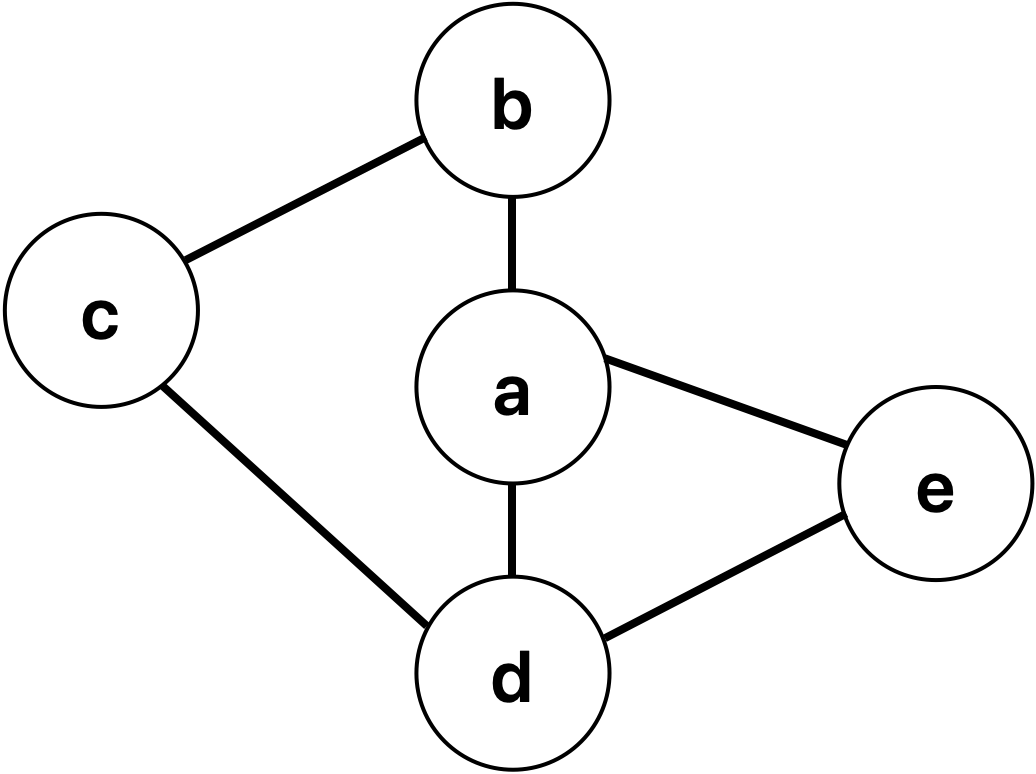
\includegraphics[width=0.7\textwidth]{assets/grafoEjemploAdj.png}
\end{figure}

\subsection{Matriz de pesos}
Cuando existe alguna propieda asociada al transporte entre nodos (usualmente distancia, costo, capacidad, etc.), estos se colocan sobre las aristas y puede expresarse en la matriz de adyacencia colocando el peso de la arista en lugar del 1, indicando así una conección y su peso correspondiente. Obsérvese un ejemplo de esto con el grafo de la Figura \ref{fig:grafEjem2} y su correspondiente matriz de adyacencia con pesos de la Tabla \ref{tab:matAdjEjem2}.
Es importante recordar que la matriz se lee en orden $ij$, es decir, el nodo $i$ conecta hacia el nodo $j$, no al revés.

\begin{figure}[H]
\centering
\caption{Ejemplo de grafo pesado dirigido.}
\label{fig:grafEjem}
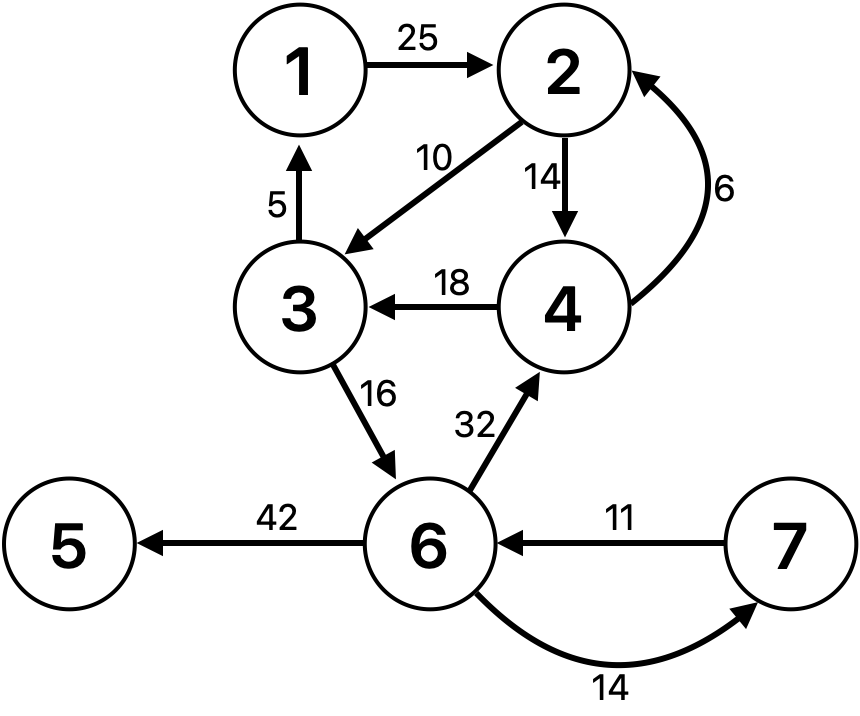
\includegraphics[width=0.7\textwidth]{assets/grafEjem2.png}
\end{figure}

\begin{table}
\centering
\caption{Matriz de adyacencia para un grafo pesado dirigido.}
\label{tab:matAdjEjem2}
\begin{tabular}{cccccccc}
&1&2&3&4&5&6&7\\
1&0&25&0&0&0&0&0\\
2&0&0&10&14&0&0&0\\
3&5&0&0&0&0&16&0\\
4&0&6&18&0&0&0&0\\
5&0&0&0&0&0&0&0\\
6&0&0&0&32&0&0&14\\
7&0&0&0&0&0&11&0
\end{tabular}
\end{table}

Conocer y entender estas repressentaciones nos es relevante, pues se utilizarán para representar y trabajar en un gran rango de problemas relacionados con la optimización en redes, como veremos en las secciones a continuación.

Dependiendo del problema y el método a utilizar para resolverlo, en la matriz de adyacencia con pesos podrá usarce un cero o el $\infty$ para indicar que no existe conección entre dos nodos $i$ e $j$.

\section{Dijkstra}
El algoritmo de Dijkstra, también llamado algoritmo de caminos mínimos, es un algoritmo para la determinación del camino más corto, dado un vértice origen, hacia el resto de los vértices en un grafo que tiene pesos en cada arista\footnote{Wikipedia: Algoritmo de Dijkstra}.

En contextos de optimización, podemos utilizarlo para calcular y minimizar distancias, costos, tiempos, etc. Veamos cómo se implementa tomando como ejemplo el grafo de la Figura \ref{fig:grafoProb10}.

\begin{figure}[H]
\centering
\caption{Grafo problema 10.}
\label{fig:grafoProb10}
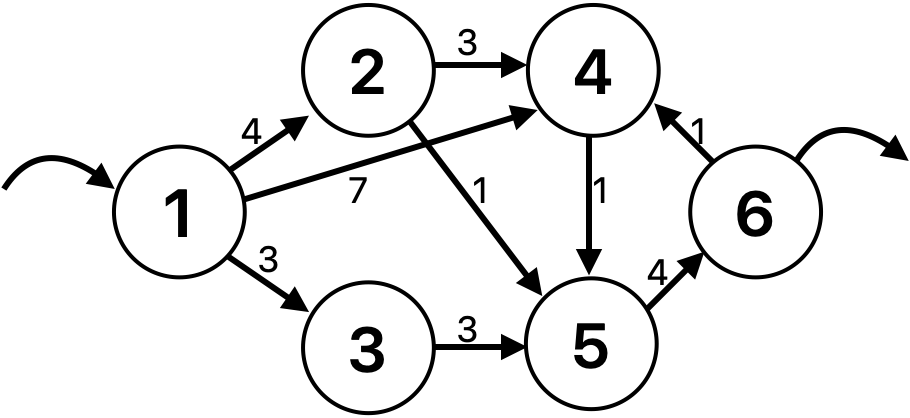
\includegraphics[width=0.7\textwidth]{assets/grafoProb10.png}
\end{figure}

\subsection{Pasos para Dijsktra}

\textbf{Paso 1.} Definir nodo origen: En el diagrama de la Figura \ref{fig:grafoProb10} el nodo origen está denotado por la flecha inicial, en este caso, el nodo 1.

\textbf{Paso 2.} Notación [Dist.origen, Nodo anterior]: Esta notación se utilizará para las etiquetas que se le asignarán a cada nodo a lo largo de la ejecución del algoritmo de Dijkstra y representan la distancia o costo desde el nodo actual hasta el nodo origen y el nodo anterior respectivamente.

\textbf{Paso 3.} Resolver un nodo: Para decir que un nodo está resuelto, necesitas haber visitado todos sus nodos vecinos, es decir, con los que tiene conexión y haber generado sus respectivas etiquetas.

\textbf{Paso 4.} Una vez resuelto un nodo, el siguiente nodo a resolver será el nodo vecino con menor costo del nodo actual. Actualizar las etiquetas de los nodos vecinos de este nuevo nodo quedandote con aquella que de una distancia o costo menor.

\textbf{Paso 5.} Repetir el paso 4 hasta haber resuelto todos los nodos, momento en que el algoritmo habrá terminado.

Para efectos de claridad, en los pasos descritos de las Figuras \ref{fig:paso1Prob10} a \ref{fig:paso6Prob10}, los nodos resueltos se marcarán en negro, los visitados en gris y los no visitados en blanco. Cuando una etiqueta de un nodo sea remplazada por otra mejor, esta se cruzará con una línea. Observemos entonces:

\begin{figure}[H]
\centering
\caption{Paso 1 Problema 10}
\label{fig:paso1Prob10}
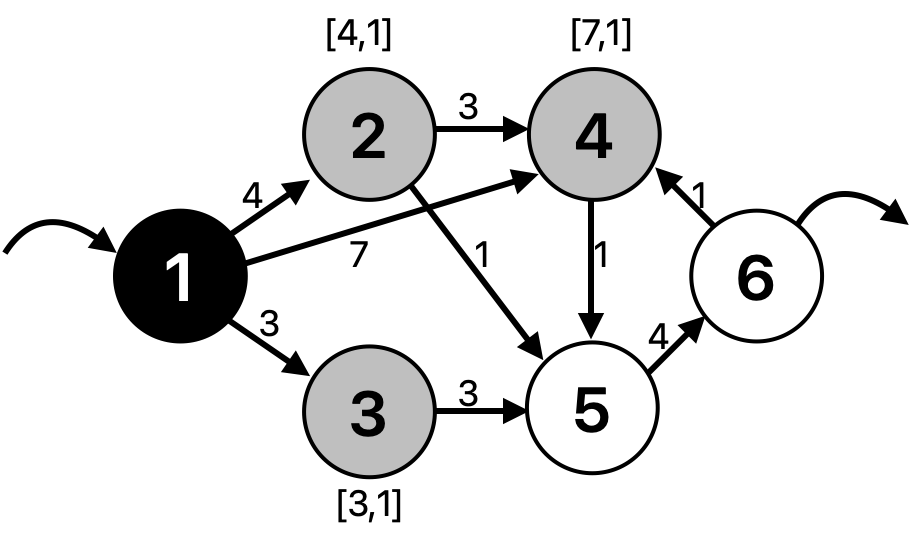
\includegraphics[width=0.7\textwidth]{assets/paso1Prob10.png}
\end{figure}

\begin{figure}[H]
\centering
\caption{Paso 2 Problema 10}
\label{fig:paso2Prob10}
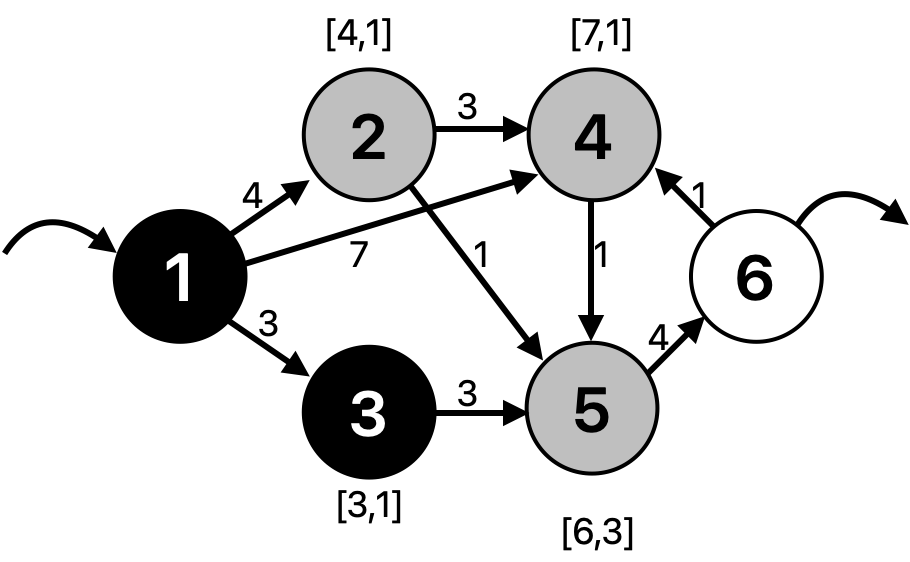
\includegraphics[width=0.7\textwidth]{assets/paso2Prob10.png}
\end{figure}

\begin{figure}[H]
\centering
\caption{Paso 3 Problema 10}
\label{fig:paso3Prob10}
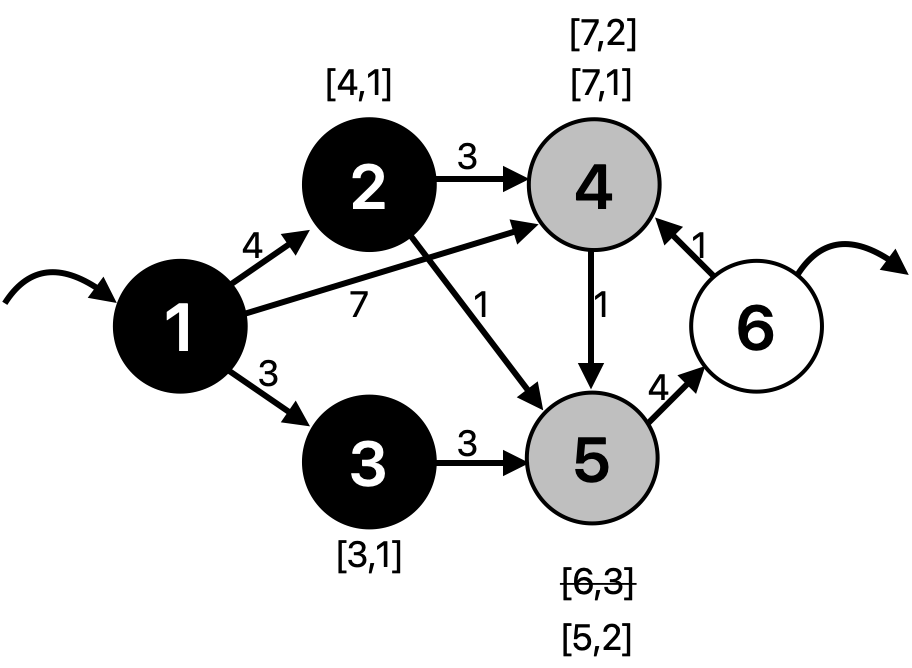
\includegraphics[width=0.7\textwidth]{assets/paso3Prob10.png}
\end{figure}

\begin{figure}[H]
\centering
\caption{Paso 4 Problema 10}
\label{fig:paso4Prob10}
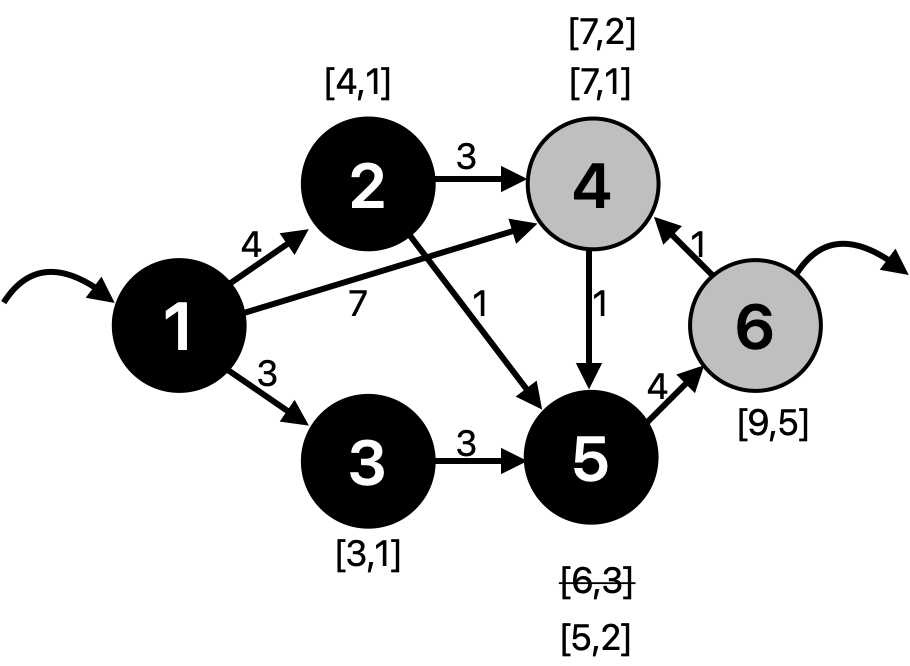
\includegraphics[width=0.7\textwidth]{assets/paso4Prob10.png}
\end{figure}

\begin{figure}[H]
\centering
\caption{Paso 5 Problema 10}
\label{fig:paso5Prob10}
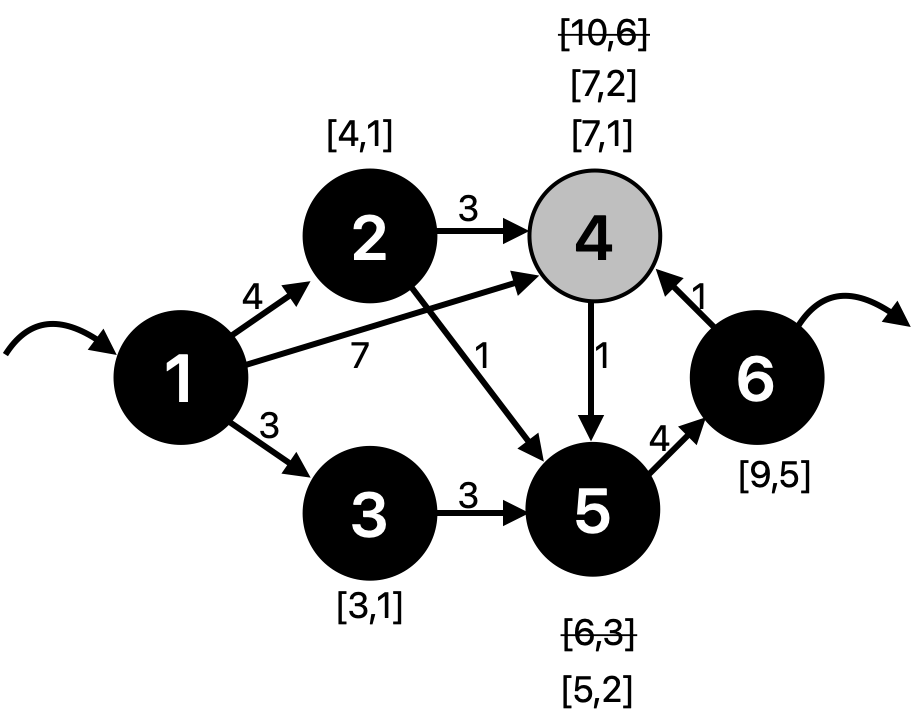
\includegraphics[width=0.7\textwidth]{assets/paso5Prob10.png}
\end{figure}

\begin{figure}[H]
\centering
\caption{Paso 6 Problema 10}
\label{fig:paso6Prob10}
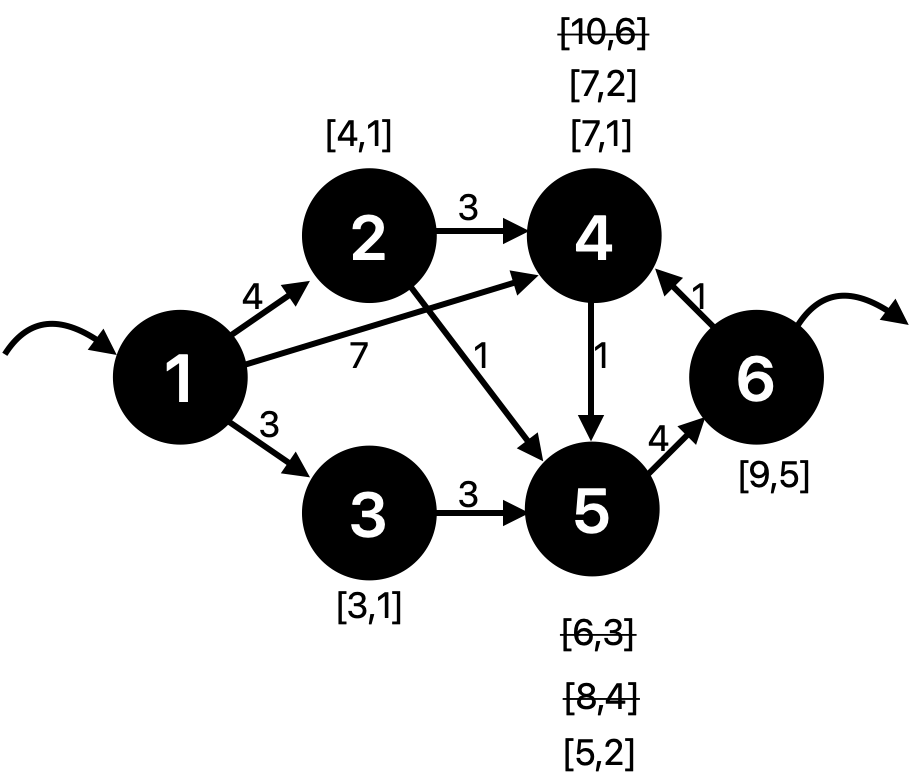
\includegraphics[width=0.7\textwidth]{assets/paso6Prob10.png}
\end{figure}

Una vez terminado el algoritmo, tendremos en las etiquetas el camino o ruta mínima desde el nodo origen a cualquier otro nodo del grafo. Si en este caso, denotamos el nodo destino como aquel con la flecha saliente (en este caso el nodo 6), entonces en su etiqueta ya tenemos el costo \mbox{total = 9} y es cuestión de recostruir el camino o ruta desde el nodo origen, como se muestra en la Figura \ref{fig:resProb10}

\begin{figure}[H]
\centering
\caption{Solución Problema 10}
\label{fig:resProb10}
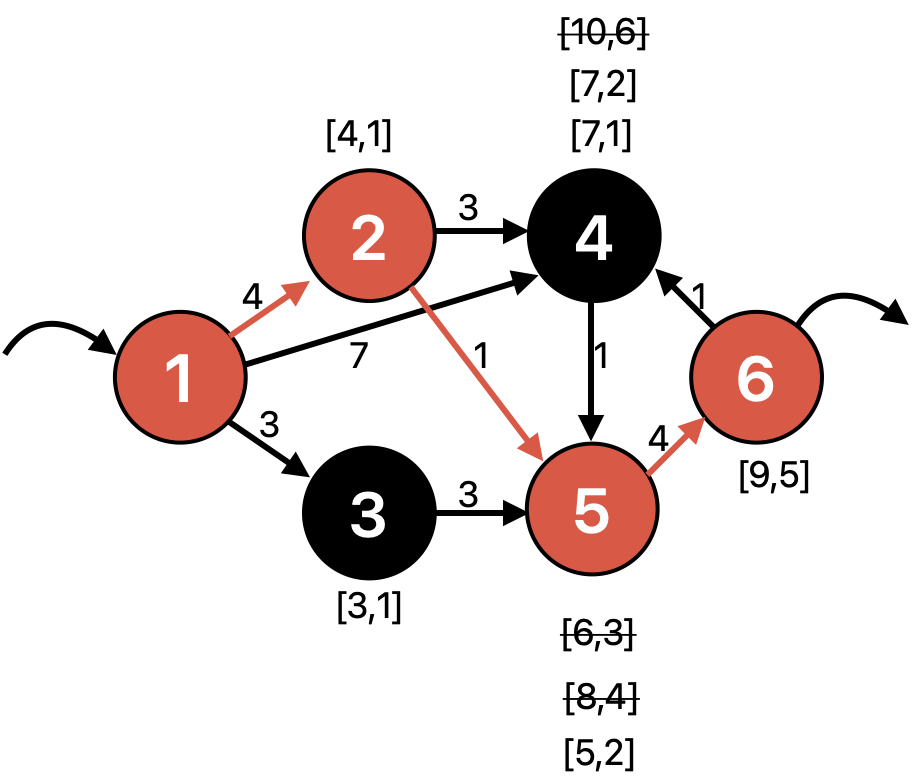
\includegraphics[width=0.7\textwidth]{assets/solProb10.png}
\end{figure}

\section{Árbol de expansión mínima: Kruskal}
El algoritmo de Kruskal se aplica a un grafo para encontrar un árbol de expansión mínima o árbol recubridor mínimo en un grafo conexo y ponderado (pesado). Es decir, busca un subconjunto de aristas que, formando un árbol, incluyen todos los nodos y donde el valor de la suma de todas las aristas del árbol es el mínimo\footnote{Wikipedia: Algoritmo de Kruskal}.

\subsection{Pasos para Kruskal}
\textbf{Paso 1.} Selecciona la arista con peso menor.

\textbf{Paso 2.} Continúa buscando y seleccionando las aristas con pesos mínimos \underline{que no generen un ciclo}.

\textbf{Paso 3.} En caso de empate, elegir cualquier arista.

\textbf{Paso 4.} Una vez unidos todos los nodos, el algoritmo termina.

Ejecutemos el algoritmo de Kruskal en el grafo de la Figura \ref{fig:grafoProb11}. Los pasos se observan de las Figuras \ref{fig:paso1Prob11} a \ref{fig:paso6Prob11} y el árbol de expansión mínima resultante se encuentra en la Figura \ref{fig:solProb11}. Veamos:

\begin{figure}[H]
\centering
\caption{Grafo para el Problema 11}
\label{fig:GrafoProb11}
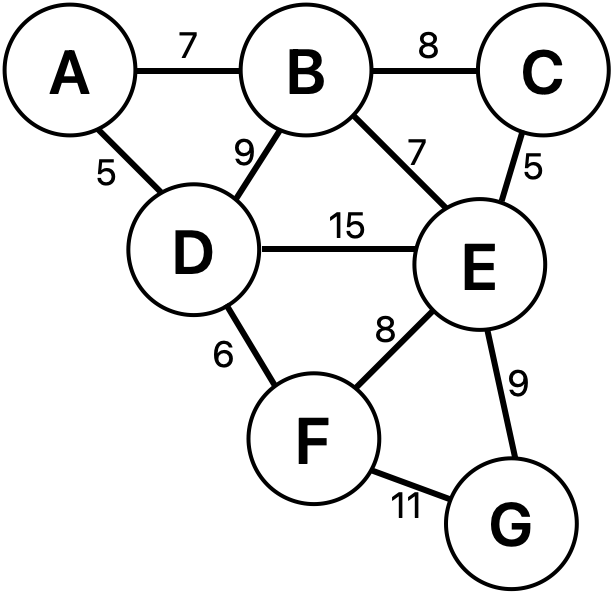
\includegraphics[width=0.6\textwidth]{assets/GrafoProb11.png}
\end{figure}

\begin{figure}[H]
\centering
\caption{Paso 1 Problema 11}
\label{fig:paso1Prob11}
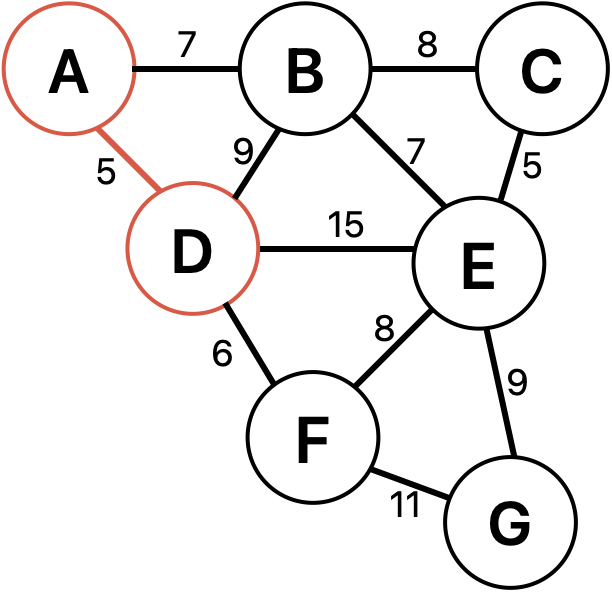
\includegraphics[width=0.6\textwidth]{assets/paso1Prob11.png}
\end{figure}

\begin{figure}[H]
\centering
\caption{Paso 2 Problema 11}
\label{fig:paso2Prob11}
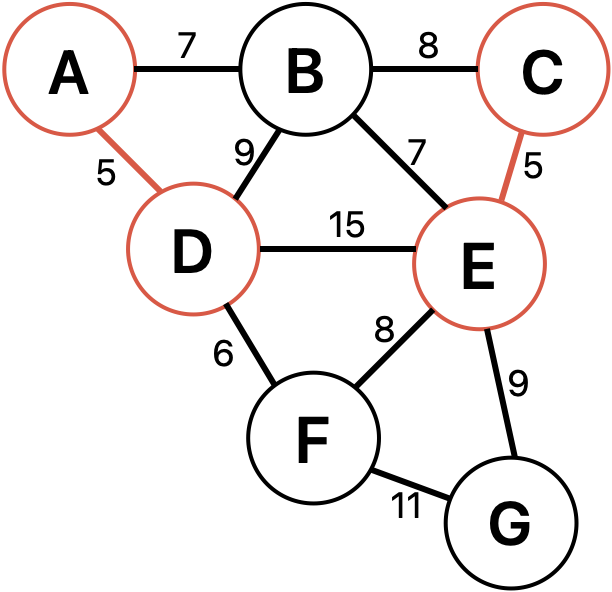
\includegraphics[width=0.6\textwidth]{assets/paso2Prob11.png}
\end{figure}

\begin{figure}[H]
\centering
\caption{Paso 3 Problema 11}
\label{fig:paso3Prob11}
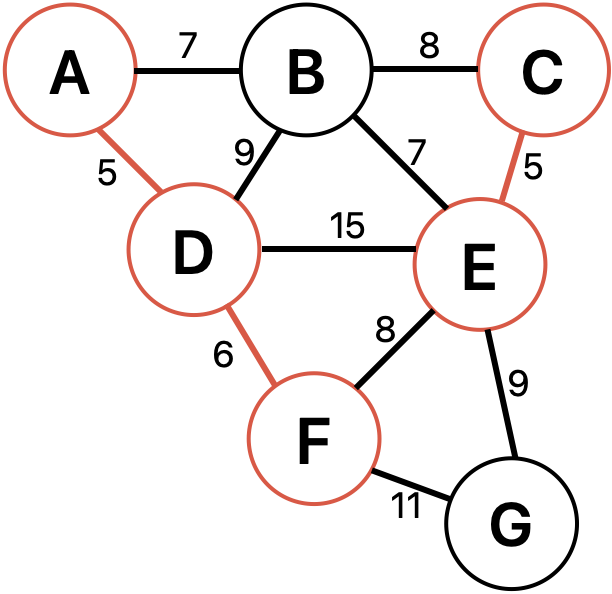
\includegraphics[width=0.6\textwidth]{assets/paso3Prob11.png}
\end{figure}

\begin{figure}[H]
\centering
\caption{Paso 4 Problema 11}
\label{fig:paso4Prob11}
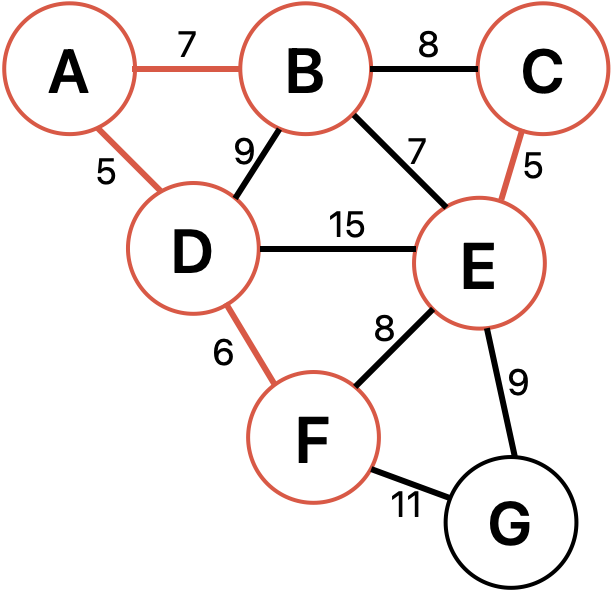
\includegraphics[width=0.6\textwidth]{assets/paso4Prob11.png}
\end{figure}

\begin{figure}[H]
\centering
\caption{Paso 5 Problema 11}
\label{fig:paso5Prob11}
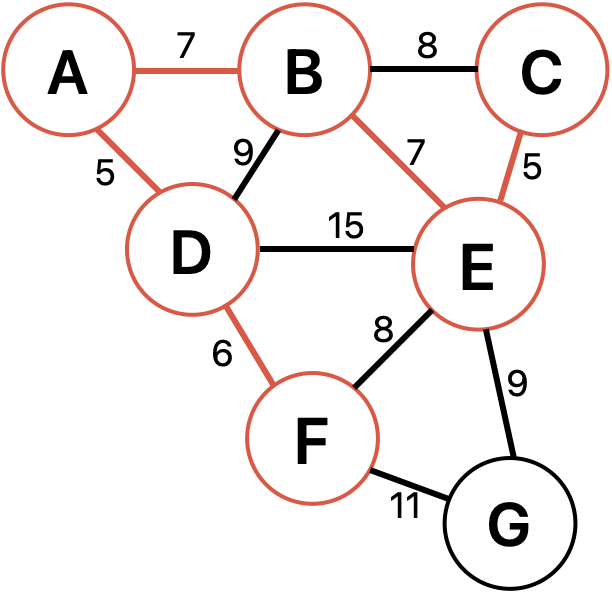
\includegraphics[width=0.6\textwidth]{assets/paso5Prob11.png}
\end{figure}

\begin{figure}[H]
\centering
\caption{Paso 6 Problema 11}
\label{fig:paso6Prob11}
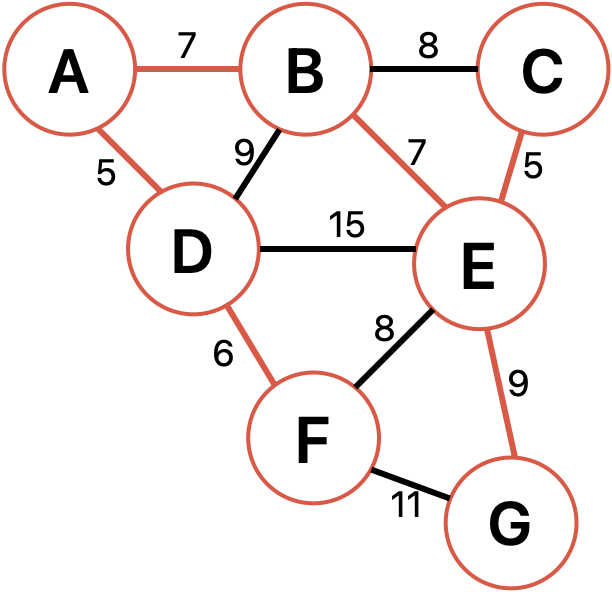
\includegraphics[width=0.6\textwidth]{assets/paso6Prob11.png}
\end{figure}

\begin{figure}[H]
\centering
\caption{Árbol de expansión mínima para el Problema 11}
\label{fig:solProb11}
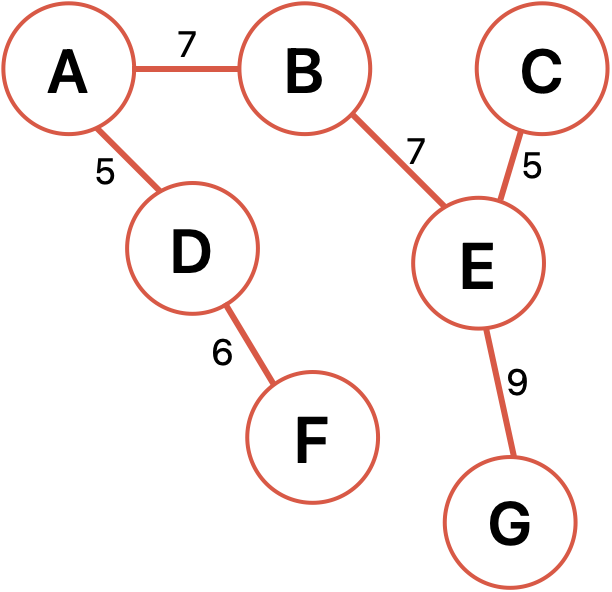
\includegraphics[width=0.6\textwidth]{assets/solProb11.png}
\end{figure}

Podemos hacer un recuento del orden en que las aristas del árbol de expansión mínima de este problema fueron seleccionadas: \{AD, CE, DF, AB, BE, EG\}.

\section{Flujo máximo: Ford-Fulkerson}
Cuando las aristas que conectan los nodos de un grafo o red tienen una capacidad máxima, la red entonces tiene una capacidad o flujo máximo asociado. Podemos calcular dicha capacidad máxima y encontrar cuellos de botella en la red, es decir, aristas que limitan la capacidad de las demás aristas.

\begin{figure}[H]
	\centering
	\caption{Modelo flujo máximo problema 12 en LINGO}
	\label{fig:lingoProb12}
	\begin{verbatim}
MODEL:
SETS:
   NODOS /1..6/;
   ARISTAS /1#2, 1#3, 2#4, 2#3, 3#5, 4#5, 4#6, 5#6/;
ENDSETS

DATA:
   CAP = @OLE(
      0   16  13   0   0   0
      0    0  10  12   0   0
      0    4   0   0  14   0
      0    0   0   0   7  20
      0    0   0   0   0   4
      0    0   0   0   0   0
   );
ENDDATA

!Variables de flujo;
VAR F(ARISTAS) >= 0;

!Función objetivo;
max = F(1,2) + F(1,3);

!Restricciones de capacidad;
F(1,2) <= 16;
F(1,3) <= 13;
F(2,4) <= 12;
F(2,3) <= 10;
F(3,5) <= 14;
F(4,5) <= 7;
F(4,6) <= 20;
F(5,6) <= 4;

!Restricciones de conservación de flujo;
F(1,2) + F(1,3) = F(2,4) + F(2,3);
F(2,4) + F(2,3) = F(3,5);
F(3,5) = F(4,5) + F(4,6);
F(4,5) + F(4,6) = F(5,6);

END
	\end{verbatim}
\end{figure}

\section{Flujo a costo mínimo}


\end{document}